\documentclass[french]{article}
\usepackage[T1]{fontenc}
\usepackage[utf8]{inputenc}
\usepackage[french]{babel}
\usepackage{amsmath}
\usepackage{mathtools}
\usepackage{color}
\usepackage[svgnames,dvipsnames]{xcolor} 
\usepackage{soul}
\usepackage{amssymb}
\usepackage{enumitem}
\usepackage{multicol}
\usepackage[left=2cm,right=2cm,top=2cm,bottom=2cm]{geometry}
\newcommand{\mathcolorbox}[2]{\colorbox{#1}{$\displaystyle #2$}}
\usepackage{pifont}
\usepackage{pst-all}
\usepackage{pstricks}
\usepackage{delarray}
\usepackage{setspace}
\usepackage{graphicx}
\usepackage{hyperref}
\usepackage{nicematrix}
\usepackage{listings}
\usepackage{float}

\hypersetup{
	colorlinks=true,
	linkcolor=blue,
	filecolor=magenta,      
	urlcolor=cyan,
	pdfpagemode=FullScreen,
}

\usepackage{amsthm}
\newtheorem*{Rem}{Remarque}

\newenvironment{conclusion}[1]{%
	\begin{center}\normalfont\textbf{Conclusion}\end{center}
	\begin{quotation} #1 \end{quotation}
}{%
	\vspace{1cm}
}

\newcommand\pythonstyle{\lstset{
	language=Python,
	basicstyle=\ttm,
	morekeywords={self},              % Add keywords here
	keywordstyle=\ttb\color{deepblue},
	emph={MyClass,__init__},          % Custom highlighting
	emphstyle=\ttb\color{deepred},    % Custom highlighting style
	stringstyle=\color{deepgreen},
	frame=tb,                         % Any extra options here
	showstringspaces=false
}}

\lstdefinestyle{Cpp}{
	language=C++,
	tabsize=3,
	basicstyle=\ttfamily,
	keywordstyle=\color{blue}\ttfamily,
	stringstyle=\color{red}\ttfamily,
	commentstyle=\color{green}\ttfamily,
	morecomment=[l][\color{magenta}]{\#}
}

\lstdefinestyle{Python}{
	language=Python,
	tabsize=3,
	basicstyle=\ttfamily,
	keywordstyle=\color{blue}\ttfamily,
	stringstyle=\color{red}\ttfamily,
	commentstyle=\color{ForestGreen}\ttfamily,
	morecomment=[l][\color{ForestGreen}]{\#}
}

\lstset{style=Cpp}

\usepackage{fontawesome}

\newcommand\numberthis{\addtocounter{equation}{1}\tag{\theequation}}

\begin{document}
	LECOURTIER Frédérique \hfill \today
	\begin{center}
		\Large\textbf{{Suivi Stage PhiFEM : 06/02/2023 - 28/07/2023}}\\
	\end{center}
	\tableofcontents
	\newpage
	
	\section{Semaine 1 : 06/02/2023 - 10/02/2023}
\graphicspath{{semaines/semaine_1/images/}}

\begin{abstract}
	Pendant cette première semaine, j'ai du me familiariser avec le code "phifem" écrit par Vincent Vigon et les codes de génération des données fournit par Killian. L'idée étant de comprendre comment générer les données avec FEniCS pour ensuite les faire apprendre par un FNO. Après la réunion du 07/02, il semblerait que le sujet du stage porte sur l'entrainement d'un FNO puis la correction/certification des prédictions.
\end{abstract}

\subsection{Génération des données}

Le code fournit par Killian (\href{https://colab.research.google.com/drive/1AJr5JaNs_gnbJce7zE2rfbjicwPxjdtL}{"Data\_Generation\_moving\_ellipse\_poisson"}) a pour but de faire varier la levelset. J'ai donc repris ce code afin de générer dans un premier temps les données solution d'un problème de Poisson avec condition de Dirichlet homogène (\href{https://colab.research.google.com/drive/1dHHFmfDs9XiMoT5EMKXQ1OFFKB3138c2}{"DataGen\_PhiFEM\_f\_gaussienne"}). 

On considère $\Omega$ le cercle de rayon $\sqrt{2}/4$ et de centre $(0.5,0.5)$ avec $\Phi(x,y)=-1/8+(x-1/2)^2+(y-1/2)^2$ et le domaine fictif $O=(0,1)^2$.

On souhaite résoudre 
\begin{equation*}
	\begin{cases}
		-\Delta u &= f\,, \quad \text{dans $\Omega$}\,, \\
		u &= 0\,, \quad \text{sur $\Gamma$}\,, \\
	\end{cases}
\end{equation*}
où 
$$f(x,y) = \exp\left(-\frac{(x-\mu_0)^2 + (y-\mu_1)^2}{2\sigma^2}\right)\,, $$ 
avec $\sigma \sim \mathcal{U}([0.1,0.6])$ et $\mu_0, \mu_1 \sim \mathcal{U}([0.5-\sqrt{2}/4, 0.5+\sqrt{2}/4])$ à condition que $\phi(\mu_0, \mu_1) < -0.05$. 

\begin{minipage}{0.48\linewidth}
	\centering
	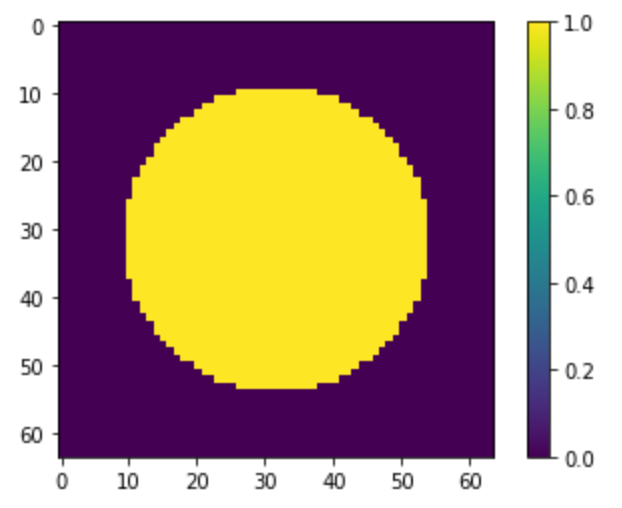
\includegraphics[width=0.5\linewidth]{domaine.png}
\end{minipage}
\begin{minipage}{0.48\linewidth}
	\centering
	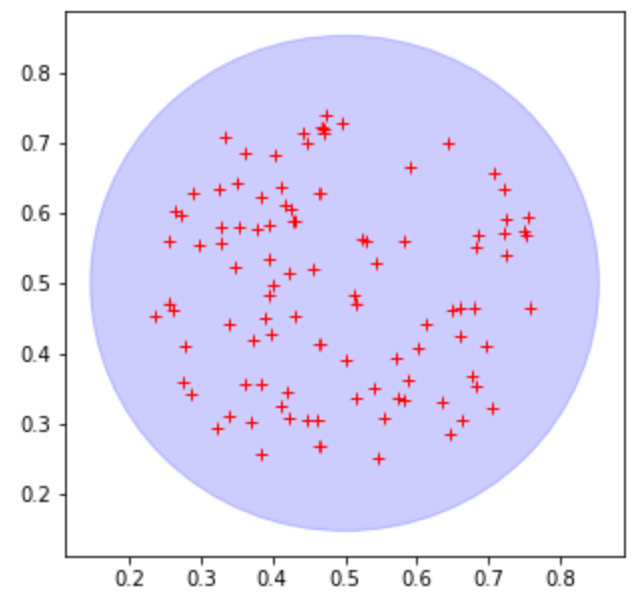
\includegraphics[width=0.45\linewidth]{parametres.png}
\end{minipage}

La fonction \textit{create\_data} renvoie le nombre donné de $F$ et les paramètres associés choisis uniformément. 

\textbf{Formulation faible :}
$$\int_{\Omega_h}\nabla(\bar{\phi}w)\nabla(\bar{\phi}v)-\int_{\partial\Omega_h}\frac{\partial}{\partial n}(\bar{\phi}w)\bar{\phi}v+G_h(w,v)=\int_{\Omega_h}f\bar{\phi}v+G_h^{rhs}(v)$$
avec
$$G_h(w,v)=\sigma h\sum_{E\in\mathcal{F}_h^\Gamma}\int_E\left[\frac{\partial}{\partial n}(\bar{\phi}w)\right]\left[\frac{\partial}{\partial n}(\bar{\phi}v)\right]+\sigma h^2\sum_{T\in\mathcal{T}_h^\Gamma}\int_T \Delta(\bar{\phi}w)\Delta(\bar{\phi}v)$$
et
$$G_h^{rhs}(v)=-\sigma h^2\sum_{T\in\mathcal{T}_h^\Gamma}\int_T f\Delta(\bar{\phi}v)$$

On utilise \href{https://fenicsproject.org/}{FEniCS} (solveur d'EDP) pour résoudre le problème. 

On va finalement stocker les résultats au format npy dans les fichiers "F.npy", "agentParams.npy" et "U.npy"

\newpage

\subsection{FNO}

De la même manière que pour la génération des données, il a fallu reprendre le code de Vincent Vigon (\href{https://colab.research.google.com/drive/1dOIb8N1i6FWXZPOvuP8xFIxmf0kjQysR}{"phifem"}) afin de l'adapter au problème considéré (\href{https://colab.research.google.com/drive/1-OdXA3xj5_X-xwvYplRStopU1yQe7AOg}{phifem\_f\_gaussienne}). 

Une première étape fut donc la lecture d'article sur les FNO (Fourier Neural Operator). Voici un schéma descriptif de ce type de réseau de neurones. 

\begin{minipage}{\linewidth}
	\centering
	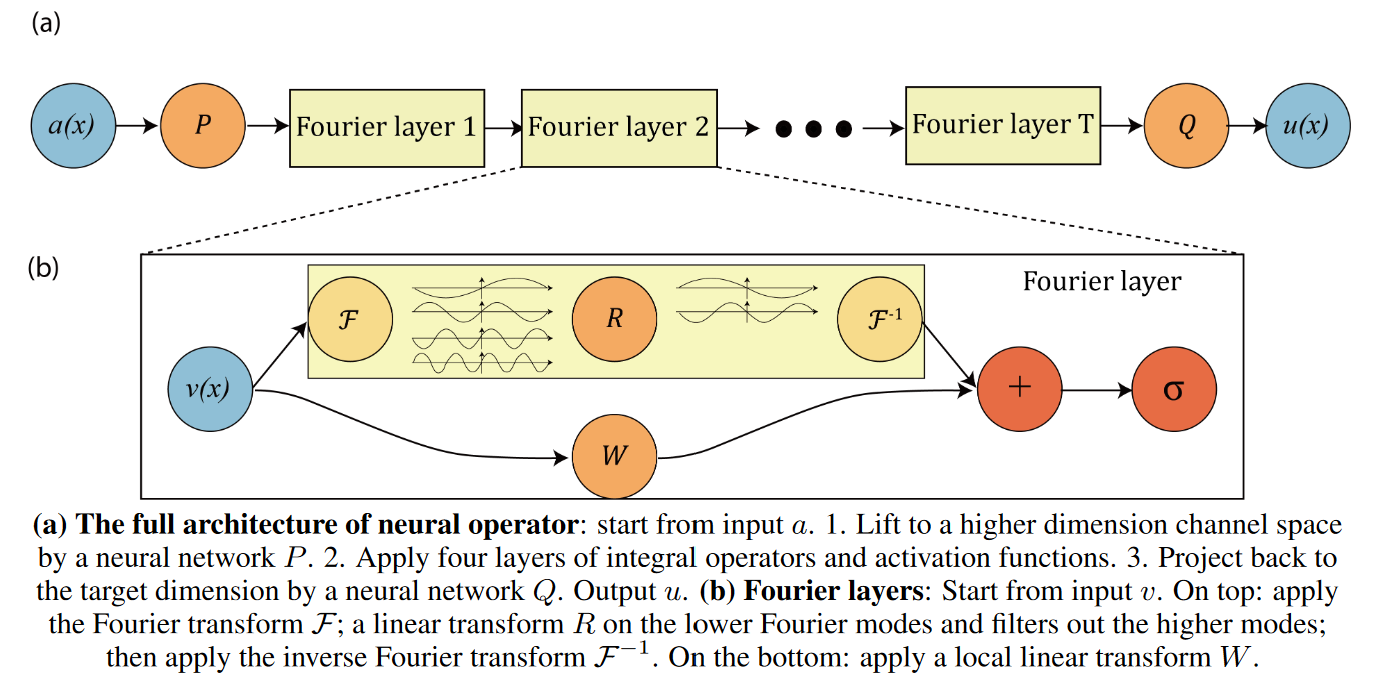
\includegraphics[width=0.7\linewidth]{FNO.png}
\end{minipage}

L'idée étant que le réseau nous retourne $u$.

\begin{Rem}
	ERREUR : il doit nous retourner $w$ car on connait déjà la levelset et pour la correction, ça n'a pas de sens de faire $\phi u=\phi^2 w$.
\end{Rem}

\subsection{Correction}

On veut en fait résoudre le même problème sauf que cette fois-ci, on définit une nouvelle levelset $\bar{\phi}=\phi u$ (où $u$ est la sortie du FNO).

On résout alors le nouveau problème $z=\bar{\phi}C$ :
\begin{equation*}
	\begin{cases}
		-\Delta z &= f\,, \quad \text{dans $\Omega$}\,, \\
		z &= 0\,, \quad \text{sur $\Gamma$}\,, \\
	\end{cases}
\end{equation*}

\begin{Rem}
	L'idée étant d'appliquer la correction sur un millage plus grossier que le réseau. Ainsi FNO+Corr plus précis que Phifem classique et plus rapide.
\end{Rem}

Les résultats obtenus (en prenant ici $u_{ex}=cos\left(\frac{\pi}{2}\times\left(\frac{4}{\sqrt{2}}\right)^2\times\left((x-0.5)^2+(y-0.5)^2\right)\right)$) ne sont pas bons :

\begin{minipage}{\linewidth}
	\centering
	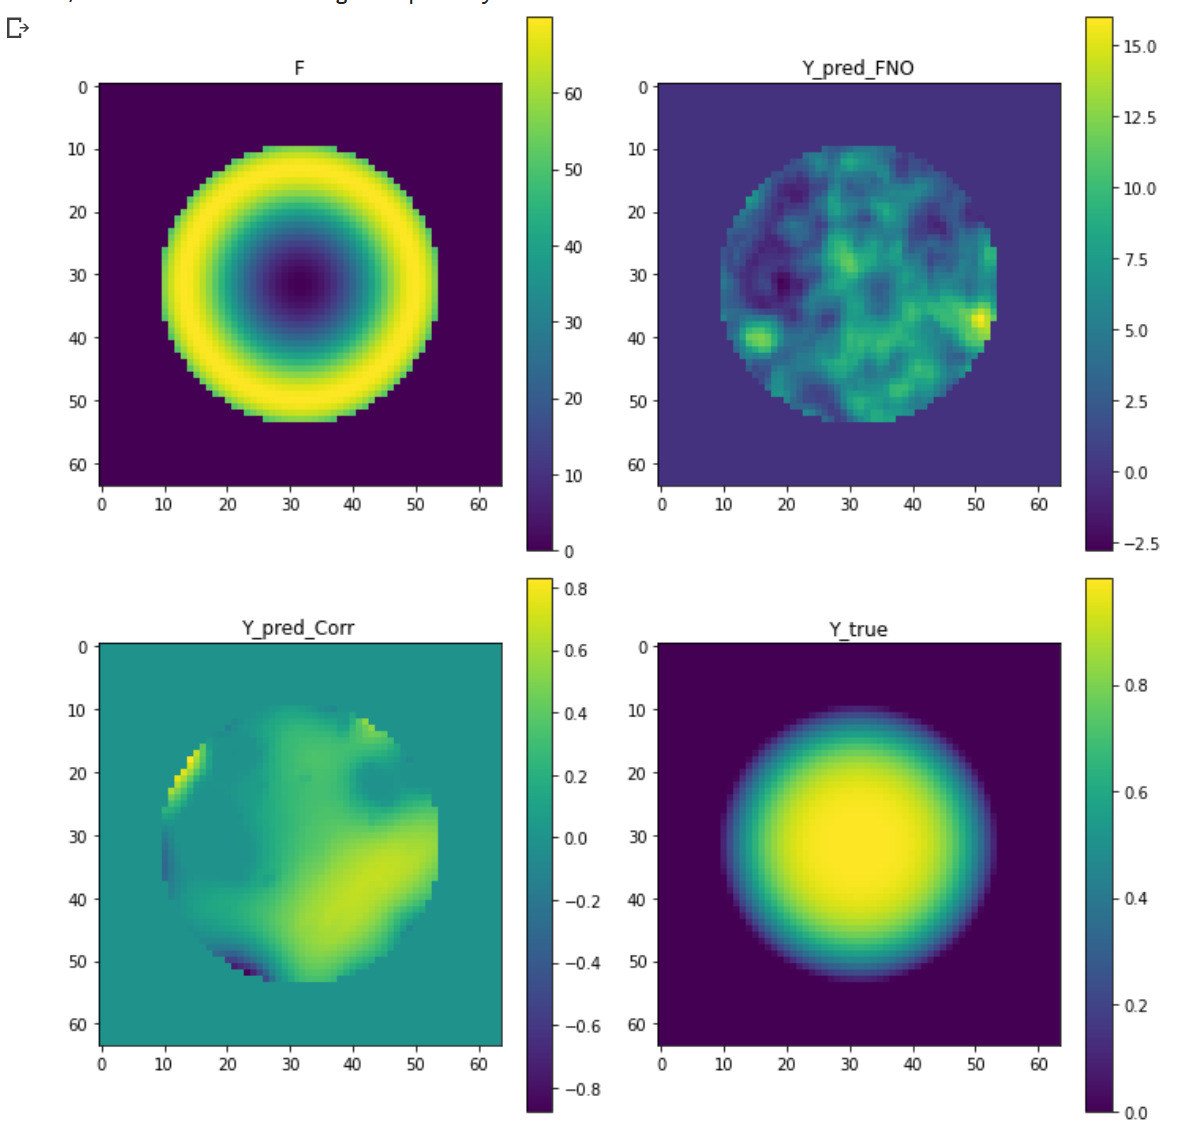
\includegraphics[width=0.45\linewidth]{resultats.png}
\end{minipage}

\begin{Rem}
	ERREUR : C'est logique !!! Le réseau n'a pas été entrainé pour ça ! (+ pb remarque d'avant.)
\end{Rem}




	
	\newpage 
	\section{Semaine 2 : 13/02/2023 - 17/02/2023}
\graphicspath{{semaines/semaine_2/images/}}

\begin{abstract}
	(Les résultats en semaine 1 ont été obtenus en début de semaine.)
	
	Après la semaine dernière, on s'est dit qu'une bonne idée serait de prendre une solution manufacturée (analytique) afin de pouvoir comparer les erreurs avec FEM classique, PhiFEM, le FNO et le FNO+correction. On a choisi de prendre $u$ comme une gaussienne et ainsi le f associé. Attention, il a fallut normaliser les F pour le FNO. On a également eut l'idée d'utiliser une solution sur-raffinée (à la place d'une solution exacte) mais ça n'a pas encore été testé.
\end{abstract}

\subsection{Génération de données}

On considère toujours $\Omega$ le cercle de rayon $\sqrt{2}/4$ et de centre $(0.5,0.5)$ avec $\Phi(x,y)=-1/8+(x-1/2)^2+(y-1/2)^2$ et le domaine fictif $O=(0,1)^2$ (\href{https://colab.research.google.com/drive/1Ymb1XZU80fwy7XxkL5_SsNs-ZVIVs3dm#scrollTo=GYtkSETwcBRp}{"DataGen\_PhiFEM\_u\_gaussienne"}).

On souhaite résoudre 
\begin{equation*}
	\begin{cases}
		-\Delta u &= f\,, \quad \text{dans $\Omega$}\,, \\
		u &= g\,, \quad \text{sur $\Gamma$}\,, \\
	\end{cases}
\end{equation*}

Notre solution analytique est
$$u_{ex}(x,y) = \exp\left(-\frac{(x-\mu_0)^2 + (y-\mu_1)^2}{2\sigma^2}\right)\,, $$ 
avec $\sigma \sim \mathcal{U}([0.1,0.6])$ et $\mu_0, \mu_1 \sim \mathcal{U}([-0.9, 0.9])$.

Ainsi 
$$f(x,y)=\left(\frac{2\sigma^2-(x-\mu_0)^2-(y-\mu_1)^2}{\sigma^4}\right)*\exp\left(-\frac{(x-\mu_0)^2 + (y-\mu_1)^2}{2\sigma^2}\right)$$
et
$$g(x,y)=u_{ex}(x,y)$$

Pour l'apprentissage du FNO, on va normaliser $f$ par $\max_f ||f||_{L^2(\Omega_h)}$

\textbf{Formulation faible :}

On utiliser une méthode directe pour inclure les conditions de Dirichlet homogène :

$$\int_{\Omega_h}\nabla(\bar{\phi}w)\nabla(\bar{\phi}v)-\int_{\partial\Omega_h}\frac{\partial}{\partial n}(\bar{\phi}w)\bar{\phi}v+G_h(w,v)=\int_{\Omega_h}f\bar{\phi}v-\left(\int_{\Omega_h}\nabla(g)\nabla(\bar{\phi}v)-\int_{\partial\Omega_h}\frac{\partial g}{\partial n}\bar{\phi}v\right)+G_h^{rhs}(v)$$
avec
$$G_h(w,v)=\sigma h\sum_{E\in\mathcal{F}_h^\Gamma}\int_E\left[\frac{\partial}{\partial n}(\bar{\phi}w)\right]\left[\frac{\partial}{\partial n}(\bar{\phi}v)\right]+\sigma h^2\sum_{T\in\mathcal{T}_h^\Gamma}\int_T \Delta(\bar{\phi}w)\Delta(\bar{\phi}v)$$
et
$$G_h^{rhs}(v)=-\sigma h^2\sum_{T\in\mathcal{T}_h^\Gamma}\int_T f\Delta(\bar{\phi}v)-\sigma h\sum_{E\in\mathcal{F}_h^\Gamma}\int_E\left[\frac{\partial g}{\partial n}\right]\left[\frac{\partial}{\partial n}(\bar{\phi}v)\right]-\sigma h^2\sum_{T\in\mathcal{T}_h^\Gamma}\int_T \Delta(g)\Delta(\bar{\phi}v)$$

\subsection{Résultat}

Voici un exemple de résultats obtenu sur $u$ une gaussienne (\href{https://colab.research.google.com/drive/1kcxNffAI2-fqmWv9swLnUrKGJRopedxF#scrollTo=oSFmuK2uVCXX}{"phifem\_u\_gaussienne"}).

\begin{minipage}{\linewidth}
	\centering
	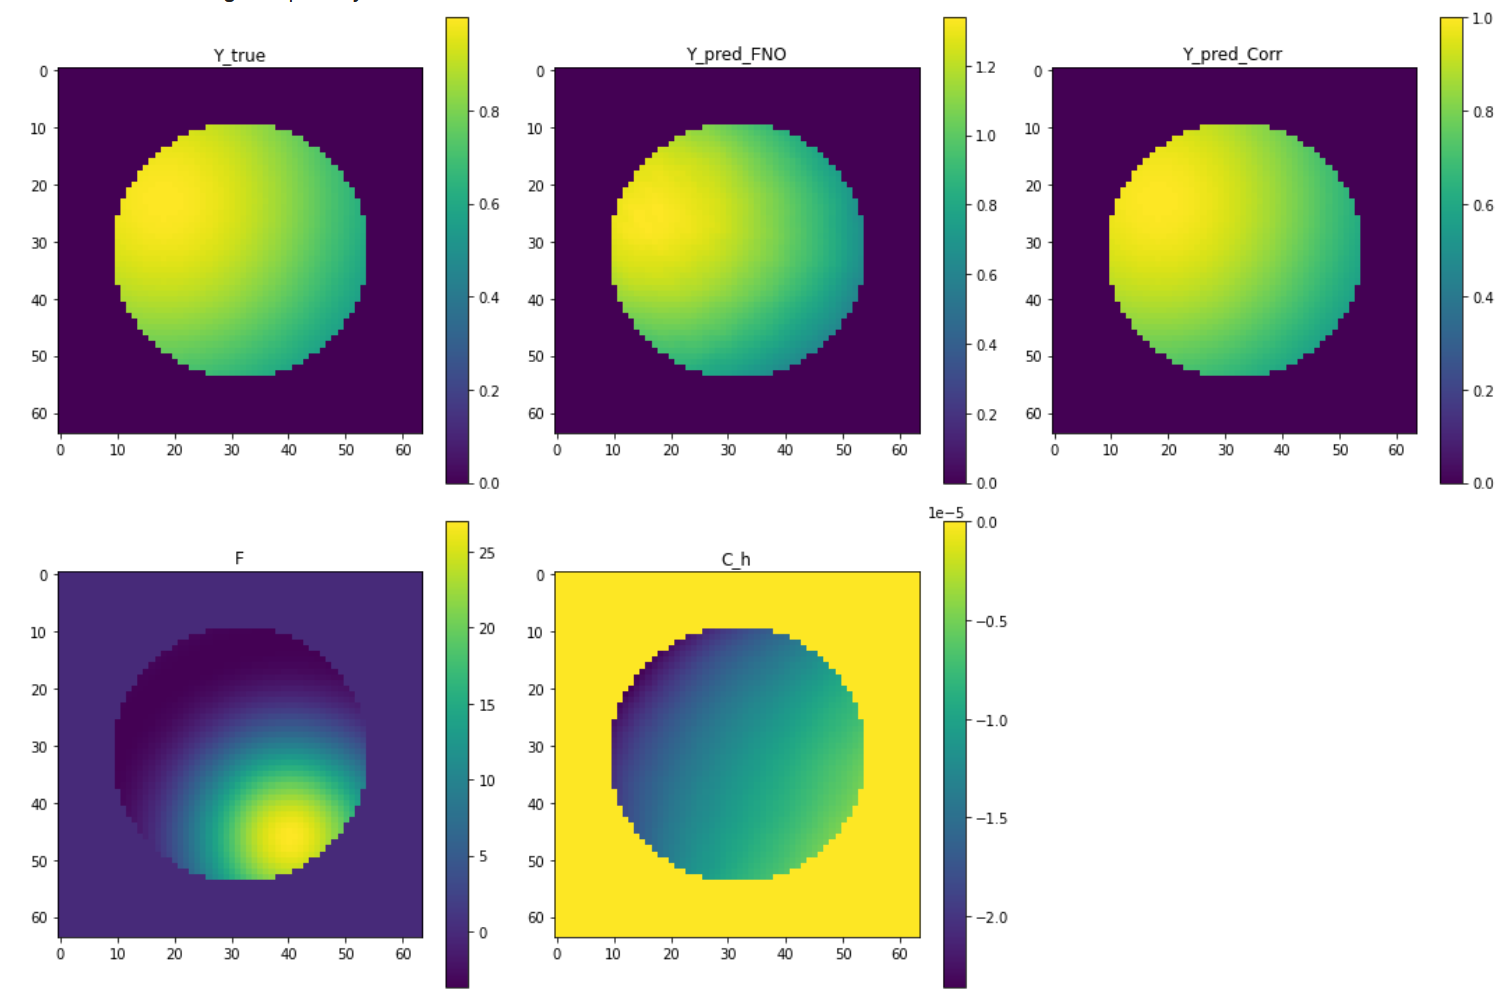
\includegraphics[width=0.45\linewidth]{resultat.png}
\end{minipage}

\conclusion{C'est en fin de semaine qu'on s'est rendue compte du problème du FNO : qu'il faut retourner $w$ et pas $u$. Les modifications ont été faites mais les résultats ne semblent toujours pas convaincant (résultats supprimés malencontreusement).
	
En fait, on a remarqué que prendre $g=u_{ex}$ sur $\Omega$ entier posait problème pour la correction, car on obtient $w=0$ et donc le problème de correction n'a plus de sens. Une solution à celà a été proposé par Emmanuel : il faudrait prendre $g=u_{ex}$ sur $\Gamma$ et étendre la solution (par exemple en utilisant un nouveau réseau de neurones qui nous fournirait une solution lisse). Mais pour l'instant, on va simplement choisir une autre solution analytique, où on n'est pas obligé de prendre $g=u_{ex}$ sur tout le domaine.

On a également eut l'idée de se ramener à un problème homogène (passage du problème en $f$ au problème en $\tilde{f}=f+\Delta g$)

Un autre problème constaté est qu'il faut utilisé le $\phi$ initial pour la génération des espaces $\mathcal{F}_h^\Gamma$ et $\mathcal{T}_h^\Gamma$.}
	
	\newpage
	\section{Semaine 3 : 20/02/2023 - 24/02/2023}
\graphicspath{{semaines/semaine_3/images/}}

\begin{abstract}
	Pour cette semaine, on considère une nouvelle solution analytique (solution trigonométrique : $\sin*\cos$). Avec cette nouvelle solution, on va pouvoir prendre g différent de $u_{ex}$ sur $\Omega$ comme souhaité pendant la semaine précédente. 
	
	A défaut de pouvoir faire tourner les entrainements (car plus d'units dispo sur colab) et en attente d'une solution avec v100, on va s'intéresser uniquement au problème de correction où on prendra comme $\bar{\phi}$ notre $u_{ex}$ ($-g$ si non homogène). En lui donnant comme nouvelle levelset notre solution exacte, $C$ doit être très proche de 1 (à l'erreur machine).  
\end{abstract}

\subsection{Génération des données}

On considère toujours $\Omega$ le cercle de rayon $\sqrt{2}/4$ et de centre $(0.5,0.5)$ avec $\Phi(x,y)=-1/8+(x-1/2)^2+(y-1/2)^2$ et le domaine fictif $O=(0,1)^2$.

On souhaite résoudre 
\begin{equation*}
	\begin{cases}
		-\Delta u &= f\,, \quad \text{dans $\Omega$}\,, \\
		u &= g\,, \quad \text{sur $\Gamma$}\,, \\
	\end{cases}
\end{equation*}

Notre solution analytique est
$$u_{ex}(x,y) = \frac{1}{\sin\left(k_1\frac{\pi}{2}\right)}\times\sin\left(k_1\frac{\pi}{2}\left(\frac{4}{\sqrt{2}}\right)^2\left((x-0.5)^2+(y-0.5)^2\right)\right)\times\cos(k_2(x^2+y^2))\,, $$ 

avec $k_1,k_2 \sim \mathcal{U}([0.1,0.5])$.

Ainsi 
$$g(x,y)=\cos(k_2(x^2+y^2))$$

On considérera également la solution analytique au problème homogène :
$$u_{ex}(x,y) = \frac{1}{\sin\left(k_1\frac{\pi}{2}\right)}\times\sin\left(k_1\frac{\pi}{2}\left(\frac{4}{\sqrt{2}}\right)^2\left((x-0.5)^2+(y-0.5)^2\right)\right)\times\cos\left(\frac{\pi}{2}\left(\frac{4}{\sqrt{2}}\right)^2\left((x-0.5)^2+(y-0.5)^2\right)\right)\,, $$ 

Les formulation faibles sont les mêmes que précédemment.

\subsection{Correction}

Dans un premier temps, on a pris notre nouvel levelset comme étant notre solution exacte sur une image 64*64 puis on interpoler cette levelset (\href{https://colab.research.google.com/drive/15rw2vTlf8yNBIuQPsFHzguUj5fmJiLf9#scrollTo=N2Z4fEjTNpAV}{"u\_trigo\_homogene"}). En prenant $\phi=u_{ex}$, on espère obtenir C très proche de 1 (en augmentant le degré d'interpolation, on espère atteindre l'erreur machine). Les résultats obtenus n'étaient pas bon :

\begin{minipage}{\linewidth}
	\centering
	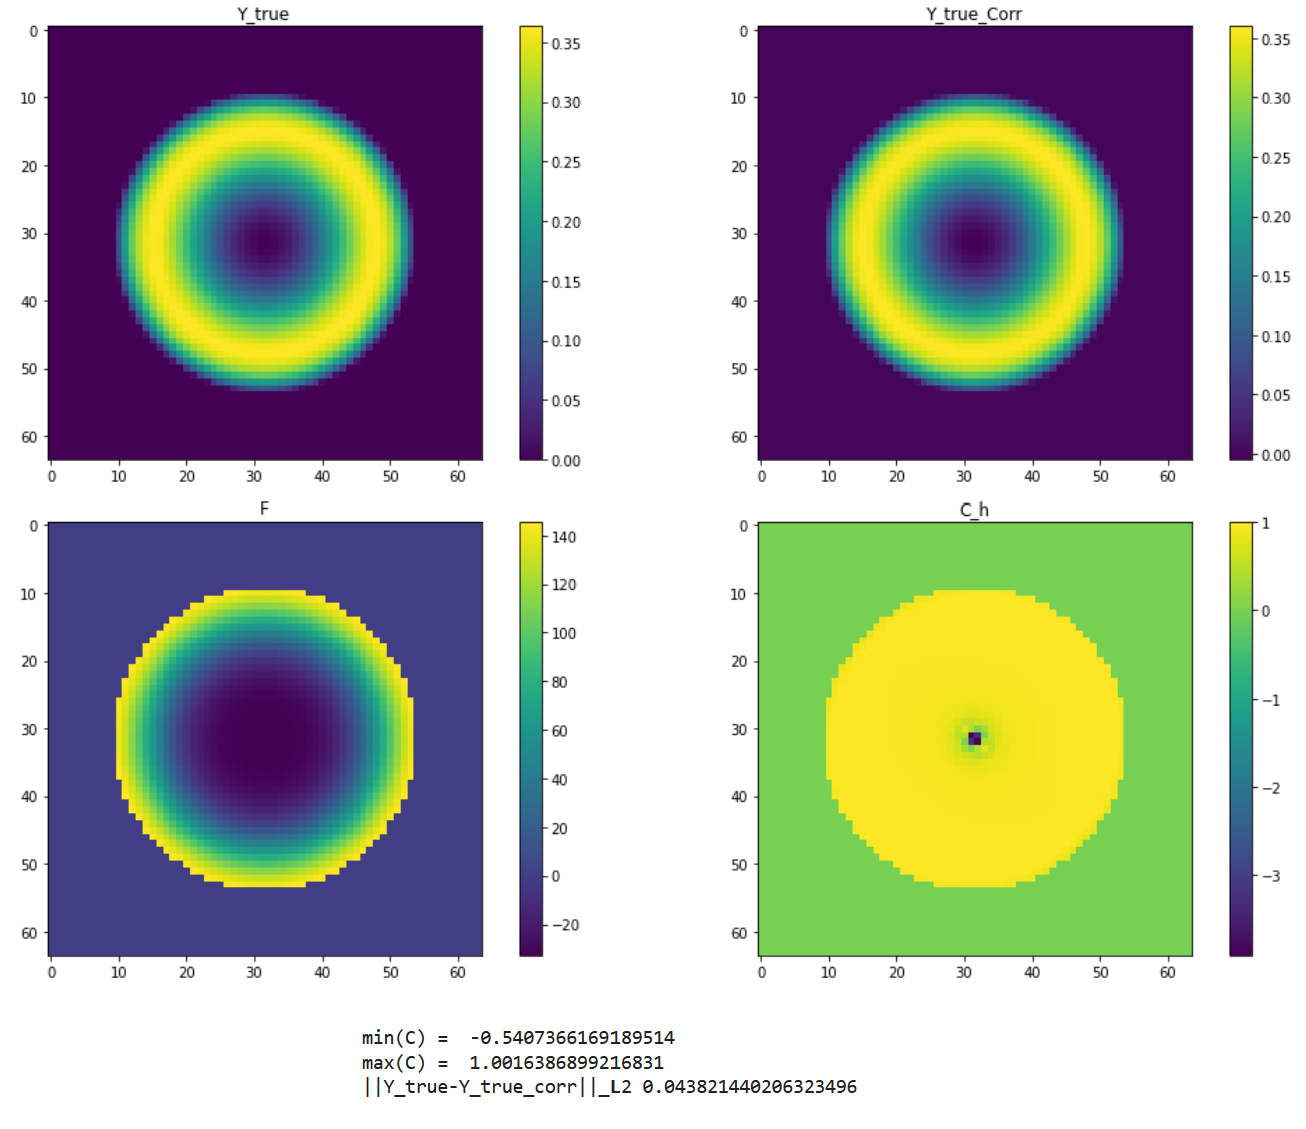
\includegraphics[width=0.45\linewidth]{resultats_correction.png}
\end{minipage}

\newpage 

En fin de semaine, on s'est rendue compte que l'interpolation de $\phi$ posait problème pour la correction. Lorsque $\bar{\phi}=u_{ex}$, on obtient bien l'erreur machine mais en lui donnant notre levelset sous la forme d'une image nb\_vert$\times$nb\_vert (ce qui est plus proche de ce que le réseau fournira), les résultats deviennent incohérents. On a donc tenter deux approches (\href{https://colab.research.google.com/drive/1JOC10OHCCNgTOCPD46bylKhlI1n1_bHR#scrollTo=0w0hQjVlLGwd}{"u\_trigo\_homogene\_modif"}): griddata (de scipy) et extrapolate (de FEniCS). L'option du extrapolate n'a pas fonctionné (nan ?). Pour l'autre option avec le griddata, on a constaté que interpoler avec tous les points de l'image était trop lourd, on a donc décidé de prendre pour chaque point (x,y) un certains nombres de points d'interpolations autour de lui. Voici les résultats obtenus avec différents nb\_vert et différents nombres de points d'interpolation :

\begin{minipage}{\linewidth}
	\centering
	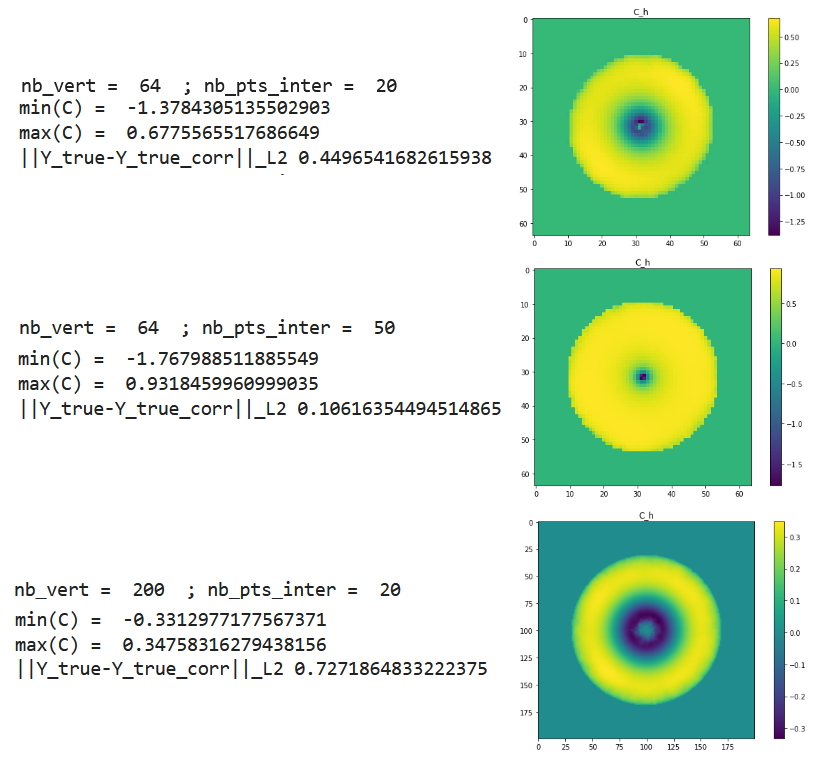
\includegraphics[width=0.6\linewidth]{griddata.png}
\end{minipage}

Ces résultats ont été obtenus la semaine suivante.


\conclusion{L'idée pour la semaine prochaine et d'effectuer quelques tests pour essayer de comprendre ce qui pose problème avec l'interpolation. Une fois ce type de problème réglé, on espère pouvoir entrainer le modèle sur la v100.}
	
	\newpage
	\section{Semaine 4 : 27/02/2023 - 03/03/2023}
\graphicspath{{semaines/semaine_4/images/}}

\begin{abstract}
	On cherche à comprendre les problèmes d'interpolation de phi dans le cadre de la correction sur la solution exacte du problème de poisson avec condition de dirichlet homogène. Après la réunion du 28/02 avec Emmanuel et Vanessa, les points suivants sont à traiter :
	\begin{enumerate}[label=\textbullet]
		\item tester avec solution analytique + perturbation !
		\item enlever les termes de stabilisation afin de voir si le problème est dans la dérivée seconde de phi
		\item visualiser le $\phi$ et le $\phi'$ EF et le comparer au $\phi$ et $\phi'$ analytique
		\item comprendre le problème du extrapolate
	\end{enumerate}
	Après la réception d'un ordinateur, on a passé la moitié de la semaine à essayer d'installer ce dont on avait besoin. En fin de semaine, les installations ont enfin été faite et je peux maintenant générer des données et entraîner le modèle sur ce nouveau PC.
\end{abstract}

\subsection{Génération des données}

On considère toujours $\Omega$ le cercle de rayon $\sqrt{2}/4$ et de centre $(0.5,0.5)$ avec $\Phi(x,y)=-1/8+(x-1/2)^2+(y-1/2)^2$ et le domaine fictif $O=(0,1)^2$.

On souhaite résoudre 
\begin{equation*}
	\begin{cases}
		-\Delta u &= f\,, \quad \text{dans $\Omega$}\,, \\
		u &= 0\,, \quad \text{sur $\Gamma$}\,, \\
	\end{cases}
\end{equation*}

Notre solution analytique est
$$u_{ex}(x,y) = \frac{1}{\sin\left(k_1\frac{\pi}{2}\right)}\times\sin\left(k_1\frac{\pi}{2}\left(\frac{4}{\sqrt{2}}\right)^2\left((x-0.5)^2+(y-0.5)^2\right)\right)\times\cos\left(\frac{\pi}{2}\left(\frac{4}{\sqrt{2}}\right)^2\left((x-0.5)^2+(y-0.5)^2\right)\right)\,, $$ 

avec $k_1 \sim \mathcal{U}([0.1,0.5])$.

\subsection{Correction}

On cherche à comprendre les problèmes d'interpolation de phi dans le cadre de la correction sur la solution exacte du problème de poisson avec condition de Dirichlet homogène (\href{https://colab.research.google.com/drive/17S0TrfstBv8vk6KR3uAy8gbeOcSkWPsY#scrollTo=7i8HL9-JKfEj}{"tests\_interpolation"}). On va effectuer plusieurs tests :

\subsubsection*{Solution analytique + Perturbation.}

Pour simuler la solution fournit par le FNO on va considérer comme nouvelle level-set notre solution analytique plus une petite perturbation. La perturbation choisie est définie par :
$$P(x,y)=\epsilon\times\sin(k_1(x+y))\times\cos(4\pi((x-0.5)^2+(y-0.5)^2))$$
On a alors
$$\Phi(x,y)=u_{ex}(x,y)+P(x,y)$$
En prenant $\epsilon=1$, on a :

\begin{minipage}{\linewidth}
	\centering
	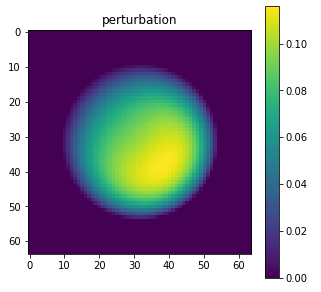
\includegraphics[width=0.3\linewidth]{perturbation.png}
\end{minipage}

On obtient en normes $L_2$ les différentes erreurs en fonction de $\epsilon=1e-k$ entre la solution initiale fournit $\Phi$ et le solution après correction $\Phi C$ : 

\begin{minipage}{\linewidth}
	\centering
	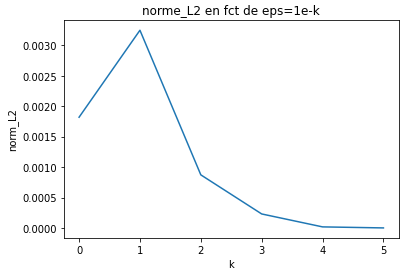
\includegraphics[width=0.45\linewidth]{erreurs_perturb.png}
\end{minipage}

Il semblerait que plus la perturbation est petite et plus l'erreur est petite. De plus, $C$ est de plus en plus proche de 1 :

\begin{minipage}{\linewidth}
	\centering
	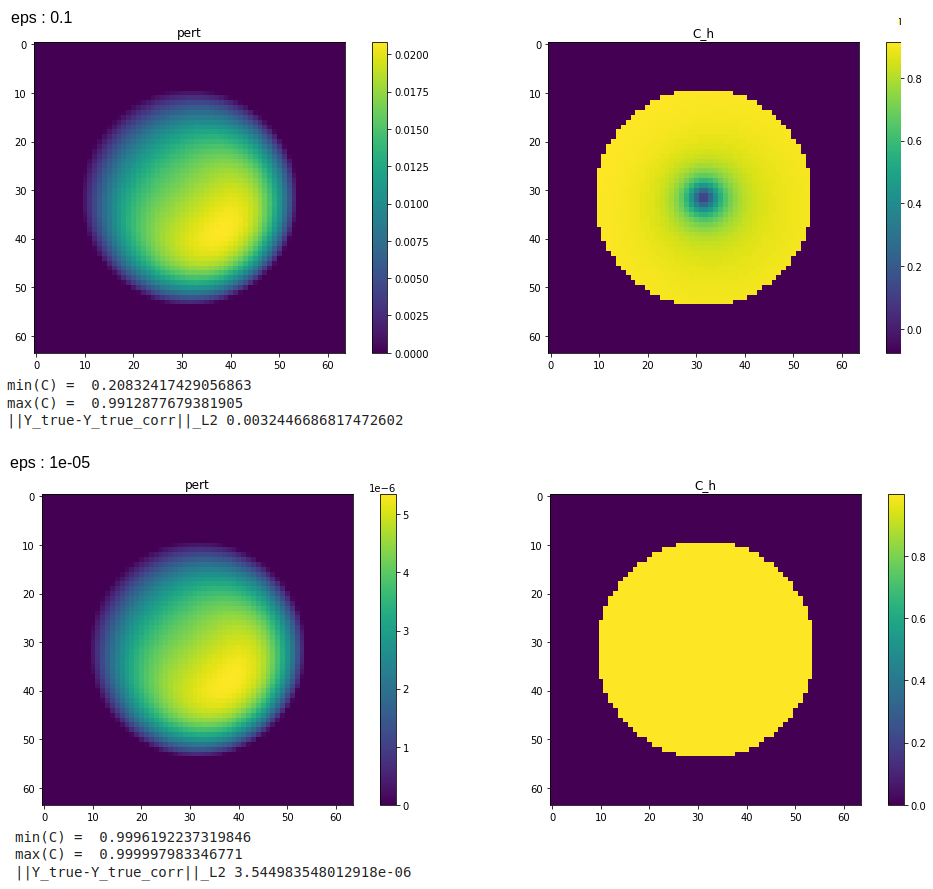
\includegraphics[width=0.55\linewidth]{results_perturb.png}
\end{minipage}

\subsubsection*{Griddata}

On a comparé $\Phi$ exact et notre $\Phi$ interpolé avec griddata (pour nb\_vert=64 et nb\_pts=20). Voici les résultats obtenus :

\begin{minipage}{\linewidth}
	\centering
	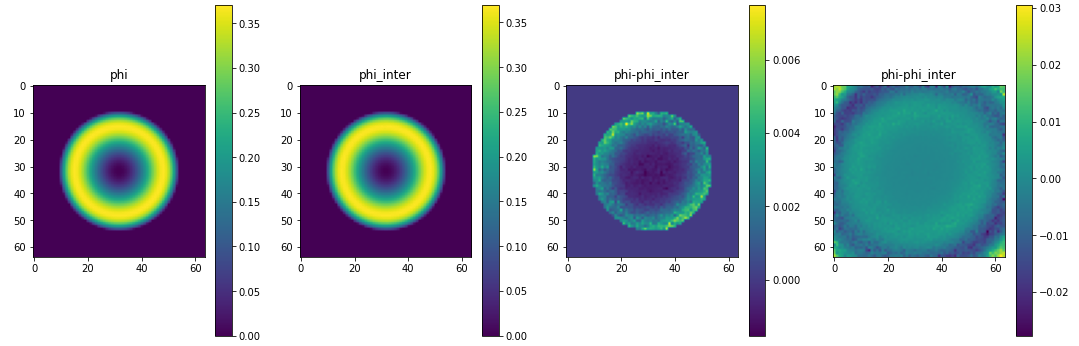
\includegraphics[width=0.9\linewidth]{results_griddata.png}
\end{minipage}

Il semblerait que sur le bord du cercle, les résultats soit moins bons. On a pas cherché à comprendre plus loin car on va utiliser la fonction extrapolate de FEniCS.


\subsubsection*{Extrapolate de FEniCS}

En milieu de semaine, on s'est rendu compte que le problème avec la foncion extrapolate que l'on avai eut la semaine dernière était que l'on pouvait n'incrémenter le degré d'interpolation que de 1.

\begin{minipage}{\linewidth}
	\centering
	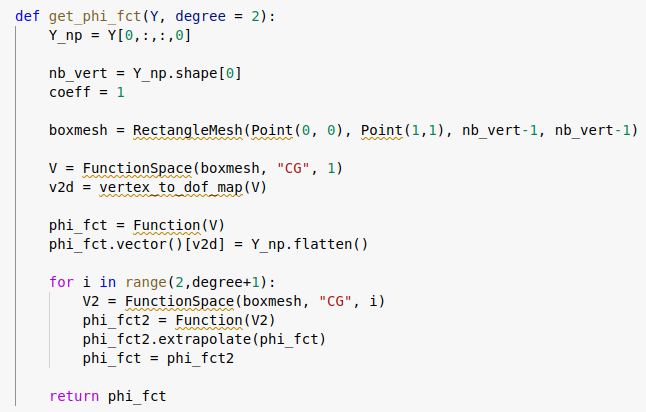
\includegraphics[width=0.5\linewidth]{get_phi_fct.png}
\end{minipage}

Voici les résultats obtenus pour une degré 2 :

\begin{minipage}{\linewidth}
	\centering
	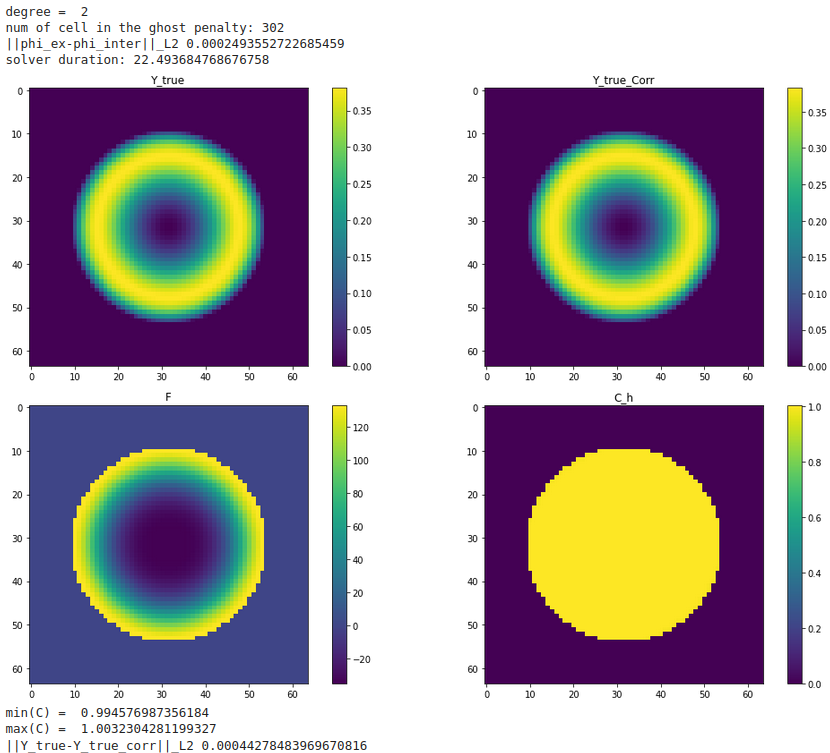
\includegraphics[width=0.9\linewidth]{results_extrapolate.png}
\end{minipage}


\conclusion{La semaine prochaine, on peut enfin entraîner le modèle car les installations ont été faites sur le nouveau pc.}

	
	\newpage
	\section{Semaine 5 : 06/03/2023 - 10/03/2023}
\graphicspath{{semaines/semaine_5/images/}}

\begin{abstract}
	Pendant cette semaine, on a globalement cherché à comprendre les problèmes liés à l'interpolation de $\phi$. On s'est donc concentré sur la précision de la correction lorsque l'on prend la solution analytique en entrée. On a testé avec deux solutions analytiques : la solution trigonométrique considérées précédemment et une solution polynomiale. La partie où l'on va utilisé le FNO sera considéré dans un second temps.
\end{abstract}

Dans toute la suite, les erreurs calculées en norme L2 sont les erreurs relatives calculées de la manière suivante :

$$||y_{true}-y_{pred}||^2_{L^2(\Omega_h),rel}=\frac{\int_{\Omega_h}(y_{true}-y_{pred})^2}{\int_{\Omega_h}y_{true}^2}$$

\subsection{Solution analytique trigonométrique}

On considère la solution analytique (au problème de Poisson avec conditions de Dirichlet homogène) :
$$u_{ex}(x,y) = \frac{1}{\sin\left(k_1\frac{\pi}{2}\right)}\times\sin\left(k_1\frac{\pi}{2}\left(\frac{4}{\sqrt{2}}\right)^2\left((x-0.5)^2+(y-0.5)^2\right)\right)\times\cos\left(\frac{\pi}{2}\left(\frac{4}{\sqrt{2}}\right)^2\left((x-0.5)^2+(y-0.5)^2\right)\right)\,, $$ 

avec $k_1 \sim \mathcal{U}([0.1,1])$.

\subsubsection*{Extrapolate en faisant varier nb\_vert}

On va calculer l'erreur en norme L2 pour différents degré d'extrapolation (de 2 à 4) et pour différents nb\_vert. On calculera les facteurs multiplicatifs entre les résultats obtenus pour différentes valeurs  de nb\_vert.

Attention : Les résultats obtenus pour chaque valeur de nb\_vert n'ont pas été calculés pour les mêmes valeurs du paramètres $k_1$. 

\begin{minipage}{\linewidth}
	\centering
	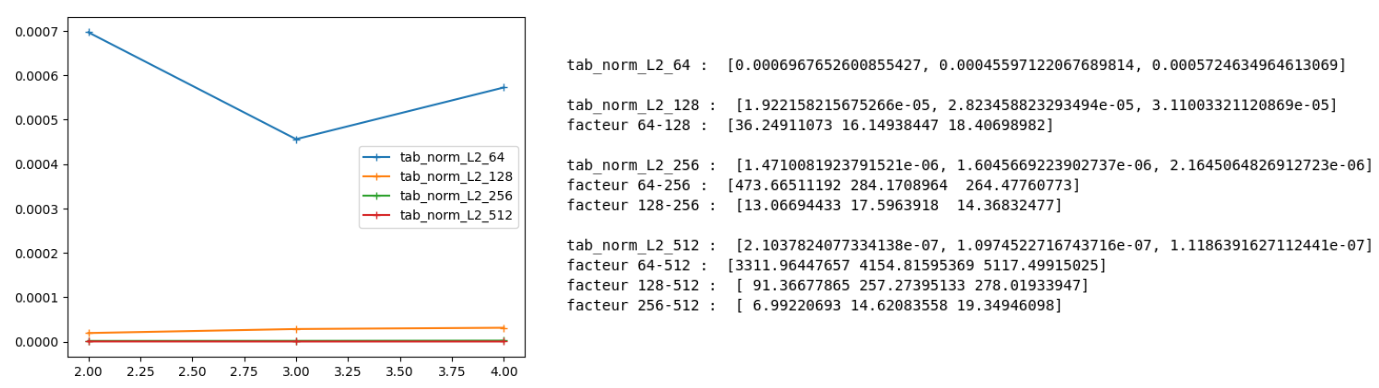
\includegraphics[width=0.9\linewidth]{test1_trigo.png}
\end{minipage}

\subsubsection*{Comparaison avec PhiFEM}

On veut comparer les erreurs en normes L2 pour différents degré d'interpolation. On fait une moyenne des résultats obtenus sur  10 valeurs de paramètres $k_1$ (nb\_data=10). Les comparaisons entre PhiFEM et la correction (pour différents degré d'interpolation) sont effectuées pour les mêmes valeurs de paramètres. On testera avec nb\_vert=64 (à gauche) et nb\_vert=128 (à droite). 

\begin{minipage}{\linewidth}
	\centering
	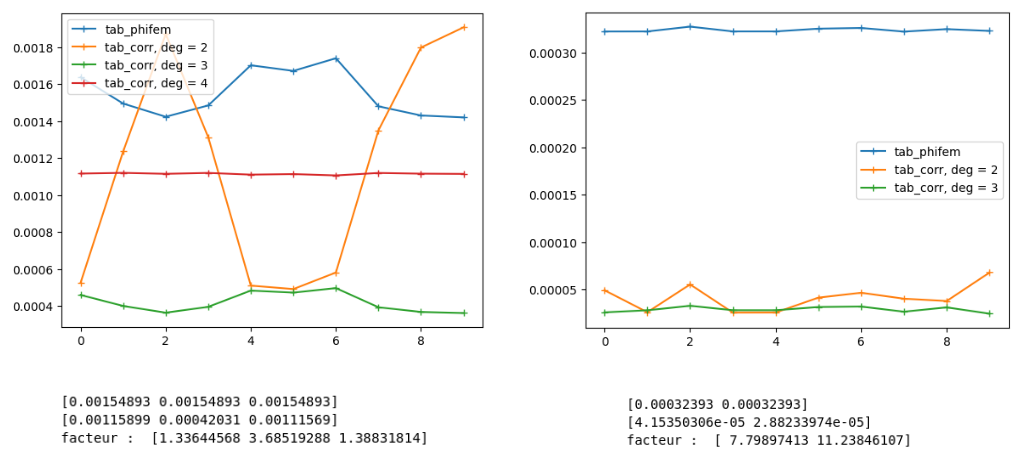
\includegraphics[width=0.7\linewidth]{test2_trigo.png}
\end{minipage}

\subsubsection*{Stratégie P1 fin -> Pk grossier}

Méthode précédente (avec le extrapolate) : On part d'une grille nb\_vert $\times$ nb\_vert. On associe alors les valeurs au noeuds aux valeurs des degré de liberté $\mathbb{P}^1$ puis on va extrapoler en $\mathbb{P}^k$ nb\_vert $\times$ nb\_vert. 

$$[\bar{\phi}=\phi w]_{ij \; grossier} \quad \longrightarrow \quad \mathbb{P}^1_{\; grossier} \quad \overset{extra}{\longrightarrow} \quad \mathbb{P}^k_{\; grossier}$$

On va considérer ici une nouvelle méthode : On part d'une grille fine nb\_vert\_fine $\times$ nb\_vert\_fine. On associe alors les valeurs aux noeuds aux valeurs des degrés de liberté $\mathbb{P}^1$ (nb\_vert\_fine $\times$ nb\_vert\_fine) puis on  interpole en $\mathbb{P}^k$ nb\_vert\_coarse $\times$ nb\_vert\_coarse. 

$$[\bar{\phi}=\phi w]_{ij \; fin} \quad \longrightarrow \quad \mathbb{P}^1_{\; fin} \quad \overset{inter}{\longrightarrow} \quad \mathbb{P}^k_{\; grossier}$$

On effectuera plusieurs comparaisons (avec nb\_data=10) :

\begin{enumerate}[label=\textbullet]
	\item \textbf{1er test : } 
	
	\begin{minipage}{0.48\linewidth}
		On va comparer les méthodes suivantes :
		$$[\bar{\phi}=\phi w]_{ij \; 64} \quad \longrightarrow \quad \mathbb{P}^1_{\; 64} \quad \overset{extra^3}{\longrightarrow} \quad \mathbb{P}^3_{\; 64}$$
		$$[\bar{\phi}=\phi w]_{ij \; 256} \quad \longrightarrow \quad \mathbb{P}^1_{\; 256} \quad \overset{inter}{\longrightarrow} \quad \mathbb{P}^2_{\; 64}$$
		$$[\bar{\phi}=\phi w]_{ij \; 256} \quad \longrightarrow \quad \mathbb{P}^1_{\; 256} \quad \overset{inter}{\longrightarrow} \quad \mathbb{P}^3_{\; 64}$$
	\end{minipage}
	\begin{minipage}{0.48\linewidth}
		\centering
		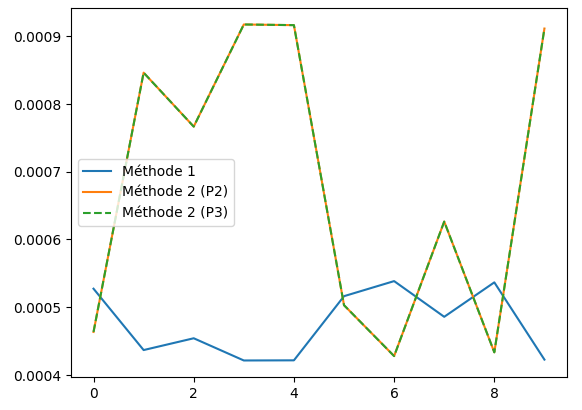
\includegraphics[width=\linewidth]{test3_trigo_1.png}
	\end{minipage}

	(Les courbes orange et verte sont très proches.)

	\item \textbf{2ème test : } 
	
	\begin{minipage}{0.48\linewidth}
		On va comparer les méthodes suivantes :
		$$[\bar{\phi}=\phi w]_{ij \; 256} \quad \longrightarrow \quad \mathbb{P}^1_{\; 256} \quad \overset{inter}{\longrightarrow} \quad \mathbb{P}^2_{\; 64}$$
		$$[\bar{\phi}=\phi w]_{ij \; 512} \quad \longrightarrow \quad \mathbb{P}^1_{\; 512} \quad \overset{inter}{\longrightarrow} \quad \mathbb{P}^3_{\; 64}$$
	\end{minipage}
	\begin{minipage}{0.48\linewidth}
		\centering
		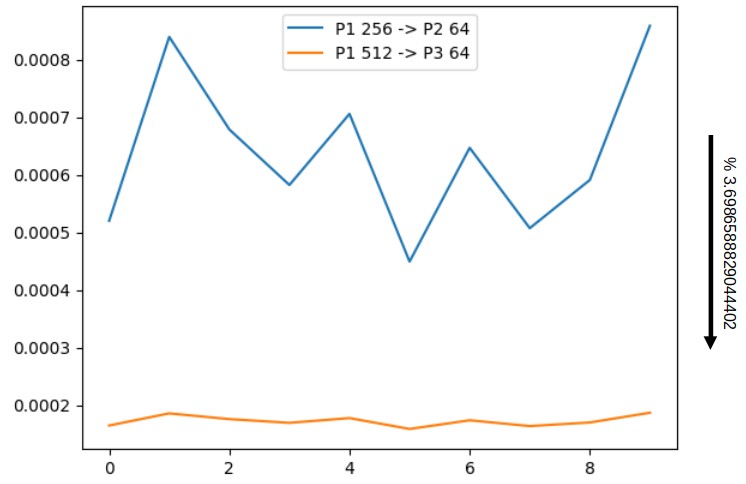
\includegraphics[width=\linewidth]{test3_trigo_2.png}
	\end{minipage}

	\item \textbf{3ème test : } 
	
	\begin{minipage}{0.48\linewidth}
		On va comparer les méthodes suivantes :
		$$[\bar{\phi}=\phi w]_{ij \; 256} \quad \longrightarrow \quad \mathbb{P}^1_{\; 256} \quad \overset{inter}{\longrightarrow} \quad \mathbb{P}^2_{\; 64}$$
		$$[\bar{\phi}=\phi w]_{ij \; 512} \quad \longrightarrow \quad \mathbb{P}^1_{\; 512} \quad \overset{inter}{\longrightarrow} \quad \mathbb{P}^3_{\; 64}$$
		$$[\bar{\phi}=\phi w]_{ij \; 512} \quad \longrightarrow \quad \mathbb{P}^1_{\; 512} \quad \overset{inter}{\longrightarrow} \quad \mathbb{P}^3_{\; 128}$$
		$$[\bar{\phi}=\phi w]_{ij \; 1024} \quad \longrightarrow \quad \mathbb{P}^1_{\; 1024} \quad \overset{inter}{\longrightarrow} \quad \mathbb{P}^3_{\; 256}$$
	\end{minipage}
	\begin{minipage}{0.48\linewidth}
		\centering
		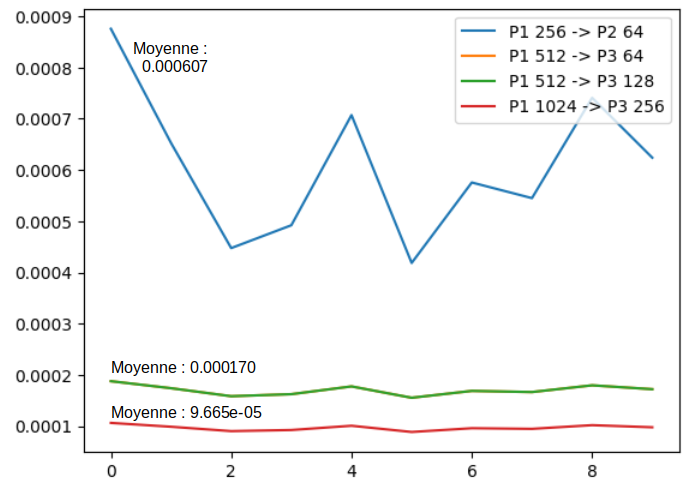
\includegraphics[width=\linewidth]{test3_trigo_3.png}
	\end{minipage}
	
	(Les courbes orange et verte sont très proches.)

\end{enumerate}

\subsection{Solution analytique polynomiale}

On considère la solution analytique (au problème de Poisson avec conditions de Dirichlet homogène) :

$$u_{ex}(x,y) = (1+k_1*x+k_2*y+x^2+y^2+x^3+y^3)\times\phi(x,y)$$

avec $k_1,k_2\sim\mathcal{U}(1,5)$

On va effectuer exactement les mêmes tests que dans le cas trigonométrique.

\subsubsection*{Extrapolate en faisant varier nb\_vert}

\begin{minipage}{\linewidth}
	\centering
	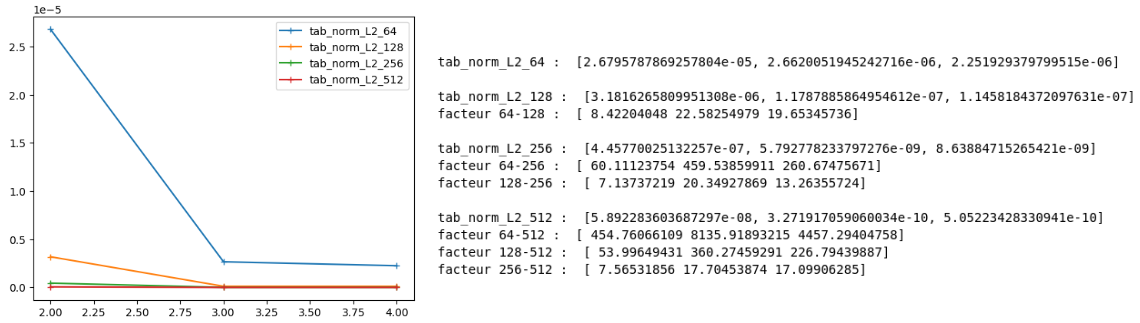
\includegraphics[width=\linewidth]{test1_poly.png}
\end{minipage}

\begin{minipage}{0.48\linewidth}
	\centering
	\subsubsection*{Comparaison avec PhiFEM}
	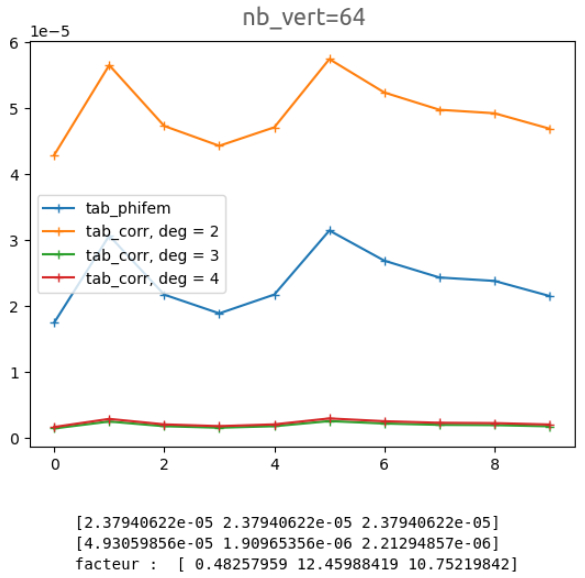
\includegraphics[width=0.85\linewidth]{test2_poly_1.png}
	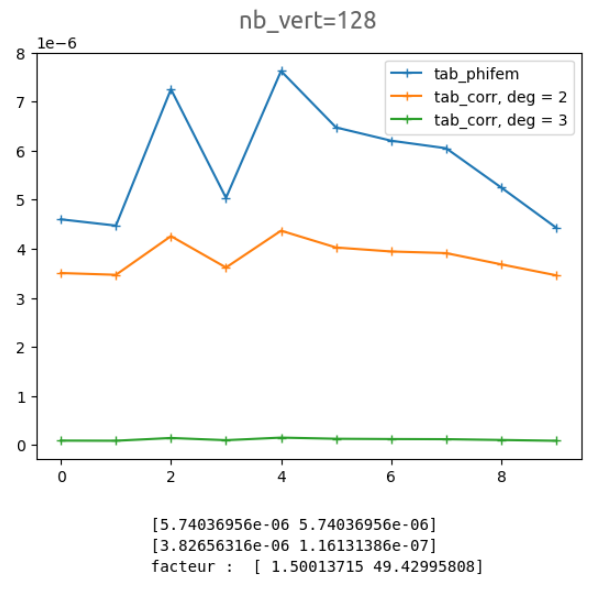
\includegraphics[width=0.85\linewidth]{test2_poly_2.png}
\end{minipage}
\begin{minipage}{0.48\linewidth}

	\centering
	\subsubsection*{Stratégie P1 fin -> Pk grossier}
	\textbf{1er test :} \\
	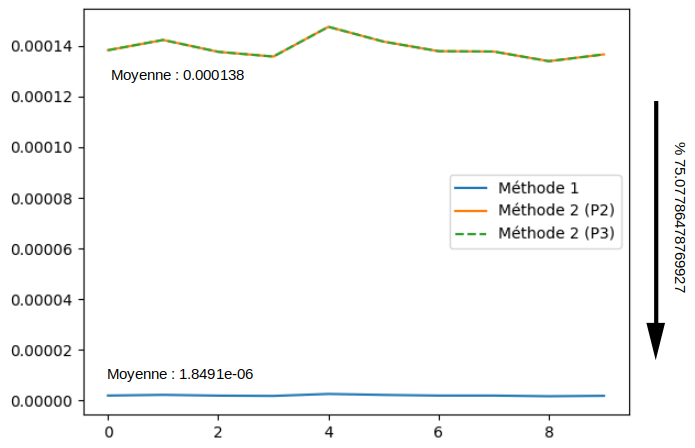
\includegraphics[width=0.8\linewidth]{test3_poly_1.png} \\
	\textbf{2ème test :} \\
	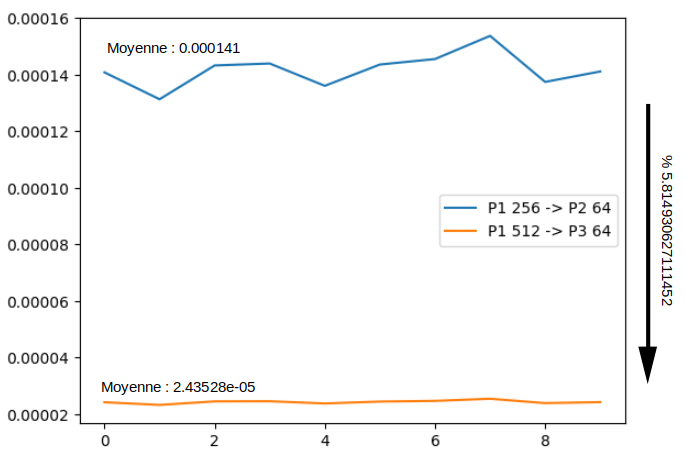
\includegraphics[width=0.8\linewidth]{test3_poly_2.png} \\
	\textbf{3ème test :} \\
	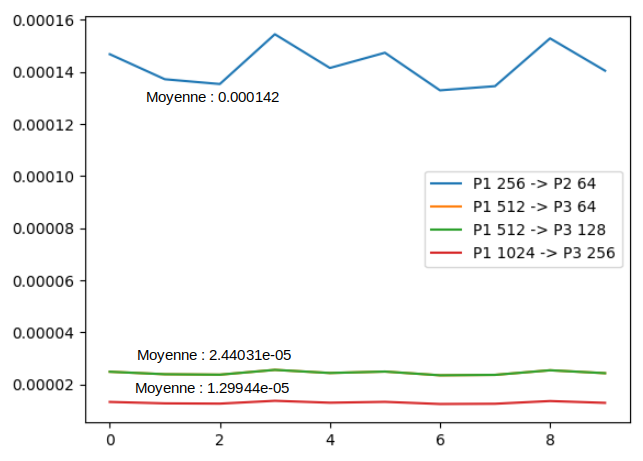
\includegraphics[width=0.7\linewidth]{test3_poly_3.png} 
\end{minipage}
	
	\newpage
	\section{Semaine 6 : 13/03/2023 - 17/03/2023}
\graphicspath{{semaines/semaine_6/images/}}


\begin{abstract}
	Après les tests de la semaine dernière sur la partie de correction/certification du modèle où l'on prend la solution analytique comme nouvelle level-set, il semblerait que la méthode avec les meilleurs résultats soit celle où l'on utilise la méthode extrapolate de FEniCS. C'est pourquoi, cette semaine on s'est intéressé en détail au code source de cette fonction FEniCS (\href{https://fenics.readthedocs.io/projects/dolfin/en/2017.2.0/apis/api_adaptivity.html#extrapolation}{Extrapolation}). Étant donné que je n'étais pas présente mardi, mercredi après-midi et jeudi car j'étais malade, c'est tout ce qui a été fait cette semaine. De plus, une grosse partie de la méthode reste encore floue : la construction de la matrice A (pour la résolution du système linéaire dans compute\_coefficients).
\end{abstract}

Pour illustrer les explications, nous considérerons un domaine rectangulaire maillés uniformément par des triangles. Dans la suite, nous considérerons également \textit{cell0} comme étant une des cellules de maillage. On prendra comme exemple une extrapolation de $\mathbb{P}^1$ vers $\mathbb{P}^2$. 

\begin{minipage}{0.48\linewidth}
	\begin{figure}[H]
		\centering
		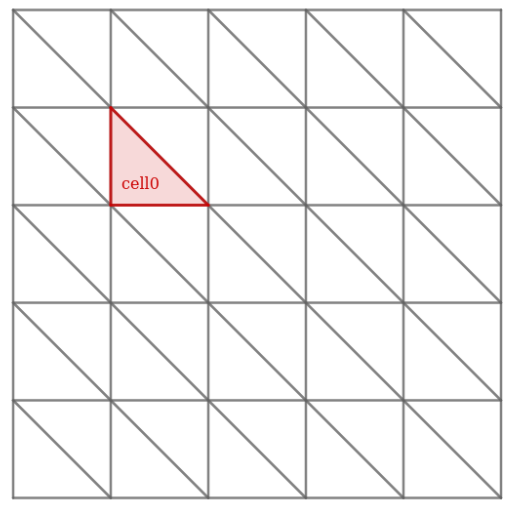
\includegraphics[width=0.5\linewidth]{cell0.png}
		\caption{Cell0}
	\end{figure}
\end{minipage}
\begin{minipage}{0.48\linewidth}
	\begin{figure}[H]
		\centering
		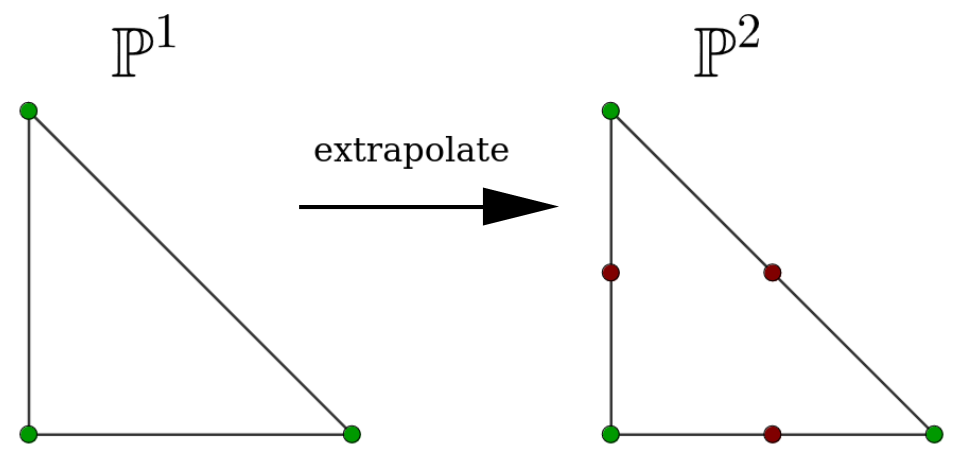
\includegraphics[width=0.9\linewidth]{P1toP2.png}
		\caption{Extrapolation de $\mathbb{P}^1$ vers $\mathbb{P}^2$}
	\end{figure}
\end{minipage} \; \\


Corps de la fonction \textbf{extrapolate} qui a pour but d'extrapoler la fonction $v$ en une fonction $w$:

\begin{lstlisting}
	void Extrapolation::extrapolate(Function& w, const Function& v)
\end{lstlisting}

On cherche à calculer la valeur en chacun des degrés de liberté associé à la fonction $w$. Pour cela, on va parcourir toutes les cellules du maillage dans le but de construire le tableau \textit{coefficients} (de taille le nombre total de degrés de liberté associés à $w$). On appelle alors sur chacune des cellules la fonction \textbf{compute\_coefficients}~\ref{compute_coefficients} qui va compléter le tableau \textit{coefficients} aux indices associées à ses degrés de liberté. Comme les degrés de liberté d'une cellule peuvent être communs à ceux d'une autre, on finira par faire une moyenne des coefficients en chacun des degrés de liberté en utilisant la fonction \textbf{average\_coefficients}~\ref{average_coefficients}, ce qui nous donne alors la fonction $w$. 

\subsection{compute\_coefficients}
\label{compute_coefficients}

Corps de la fonction :

\begin{lstlisting}
	void Extrapolation::compute_coefficients(
	std::vector<std::vector<double>>& coefficients,
	const Function& v,
	const FunctionSpace& V,
	const FunctionSpace& W,
	const Cell& cell0,
	const std::vector<double>& coordinate_dofs0,
	const ufc::cell& c0,
	const Eigen::Ref<const Eigen::Matrix<dolfin::la_index, Eigen::Dynamic, 1>> dofs,
	std::size_t& offset)
\end{lstlisting}

Cette fonction a pour but de compléter le tableau \textit{coefficients} aux indices associées aux degrés de liberté d'une cellule donnée \textit{cell0}. Autrement dit, on cherche à déterminer les valeurs aux degrés de liberté de la cellule \textit{cell0} en utilisant l'information que nous apporte les cellule voisines à celle-ci.\\

On commence par construire les tableaux \textit{cell2dof2row} et \textit{unique\_dofs} en utilisant la fonction \textbf{build\_unique\_dofs}~\ref{build_unique_dofs}. L'ensemble \textit{unique\_dofs} contient tous les degrés de liberté de notre espace de départ $V$ (associé à la fonction $v$) des cellules voisines à \textit{cell0}. Le dictionnaire \textit{cell2dof2row} permet d'associer à chaque degré de liberté (unique) d'une cellule donnée un numéro de ligne unique. 

Ensuite, on définit $N$ le nombre de degré de liberté associé à un élément de $W$ (dans notre cas $N=6$) et $M$ le nombre de degré de liberté (unique) des cellules voisines à la cellule courante \textit{cell0} (dans notre cas les nœuds des cellules voisines et donc $M=12$). Attention : il faut que $M\ge N$ pour avoir suffisamment de degré de libertés pour pouvoir construire l'extrapolation.

On peut maintenant créer la matrice $A$ (de taille $M\times N$) et le vecteur $b$ (de taille $M$). En parcourant les cellules voisines de la cellule courante \textit{cell0}, on va compléter la matrice $A$ et le vecteur $b$ en utilisant la fonction \textbf{add\_cell\_equations}~\ref{add_cell_equations}. A noter que la cellule courante \textit{cell0} est inclue dans ses cellules voisines.

On pourra ensuite résoudre le système linéaire $Ax=b$ qui nous donnera la valeur en chacun des degrés de liberté de la cellule courante \textit{cell0}. Ces valeurs sont alors ajoutées au tableau global \textit{coefficients} qui nous fournit après avoir utilisé la fonction \textbf{average\_coefficients}~\ref{average_coefficients} les valeurs en chaque degré de liberté de $w$.

\subsection{build\_unique\_dofs}
\label{build_unique_dofs}

Corps de la fonction :

\begin{lstlisting}
	void Extrapolation::build_unique_dofs(
	std::set<std::size_t>& unique_dofs,
	std::map<std::size_t, std::map<std::size_t, std::size_t>>& cell2dof2row,
	const Cell& cell0,
	const FunctionSpace& V)
\end{lstlisting}

Cette fonction a pour but de compléter les tableaux \textit{cell2dof2row} et \textit{unique\_dofs} donnés en entrée. A noter que au total, on a le même nombre de degré de liberté dans \textit{cell2dof2row} et \textit{unique\_dofs}.\\

On commence par remplir un ensemble contenant les cellules voisines à \textit{cell0}. Pour être plus précis, les cellules voisines à \textit{cell0} sont les cellules ayant un nœud commun avec la cellule courante \textit{cell0} (Figure~\ref{fig3}).

En parcourant ensuite chacune de ces cellules, on va pouvoir compléter les tableaux \textit{cell2dof2row} et \textit{unique\_dofs} donnés en entrée en appelant la fonction \textbf{compute\_unique\_dofs}~\ref{compute_unique_dofs}. 

Dans le cas de notre exemple, on va numéroter tous les nœuds des cellules voisines à \textit{cell0} et on supposera que le parcours des cellules est effectuées dans un ordre précis (Figure~\ref{fig4}).

Alors le set \textit{unique\_dofs} contiendra tous les noeuds des cellules voisines à \textit{cell0} : 
$$unique\_dofs = \{n1,n2,n3,\dots,n12\}$$

Et le dictionnaire \textit{cell2dof2row} associé à \textit{cell0} est construit de la manière suivante :
$$cell2dof2row = \begin{aligned}[t]
	\{\quad&"cell0":\{"n1":0,"n2":1,"n3":2\},&& \\
	&"cell1":\{"n4":3\}, \\
	&"cell2":\{"n5":4\}, \\
	&\dots &&\}
\end{aligned}$$

\begin{minipage}{0.48\linewidth}
	\begin{figure}[H]
		\centering
		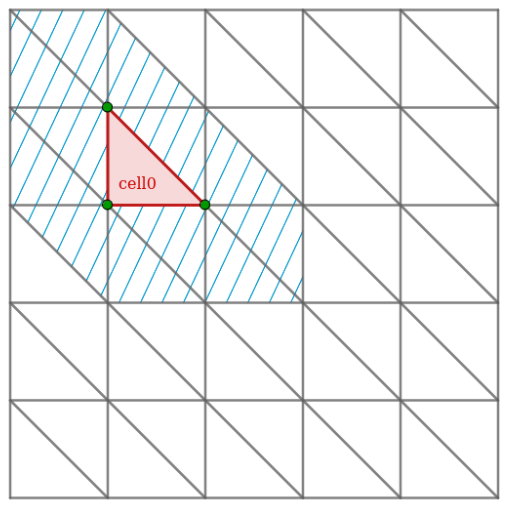
\includegraphics[width=0.6\linewidth]{surrounding_cells.png}
		\caption{Cellules voisines à Cell0}
		\label{fig3}
	\end{figure}
\end{minipage}
\begin{minipage}{0.48\linewidth}
	\begin{figure}[H]
		\centering
		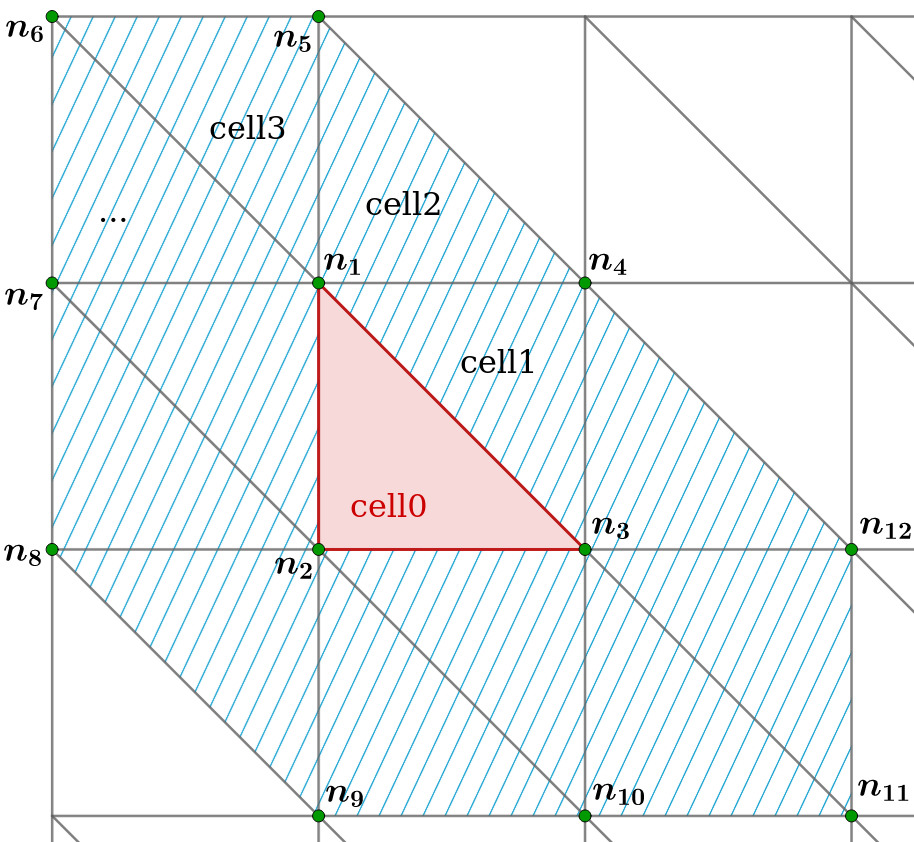
\includegraphics[width=0.6\linewidth]{cell2dof2row.png}
		\caption{Parcours des cellules voisines}
		\label{fig4}
	\end{figure}
\end{minipage}


\subsection{compute\_unique\_dofs}
\label{compute_unique_dofs}

Corps de la fonction :

\begin{lstlisting}
	std::map<std::size_t, std::size_t> Extrapolation::compute_unique_dofs(
	const Cell& cell,
	const FunctionSpace& V,
	std::size_t& row,
	std::set<std::size_t>& unique_dofs)
\end{lstlisting}

Cette fonction a pour but de traiter chacune des cellules voisines afin de compléter les tableaux \textit{unique\_dofs} et \textit{cell2dof2row} créés dans \textbf{compute\_coefficients}~\ref{compute_coefficients}.\\

Pour une cellule \textit{cell} (voisine à \textit{cell0}), on va parcourir chacun de ses degrés de liberté associé à l'espace $V$. Autrement dit, on parcourt tous les degrés de liberté dont la valeur est connue (dans notre cas les degrés de liberté $\mathbb{P}^1$ et donc les noeuds de la cellule). Si ce degré de liberté fait partie de \textit{unique\_dofs}, on ne fait rien. Sinon, on l'ajoute à \textit{unique\_dofs}. On va également créer un tableau \textit{dof2row} qui a pour but d'associer un degré de liberté à un numéro de ligne unique. Ce dictionnaire \textit{dof2row} est retourné par la fonction et permet de remplir le dictionnaire plus général \textit{cell2dof2row} créé dans \textbf{compute\_coefficients}~\ref{compute_coefficients}.

\subsection{add\_cell\_equations}
\label{add_cell_equations}

Corps de la fonction :

\begin{lstlisting}
	void Extrapolation::add_cell_equations(
	Eigen::MatrixXd& A,
	Eigen::VectorXd& b,
	const Cell& cell0,
	const Cell& cell1,
	const std::vector<double>& coordinate_dofs0,
	const std::vector<double>& coordinate_dofs1,
	const ufc::cell& c0,
	const ufc::cell& c1,
	const FunctionSpace& V,
	const FunctionSpace& W,
	const Function& v,
	std::map<std::size_t, std::size_t>& dof2row)
\end{lstlisting}

Cette fonction a pour but de remplir une partie de la matrice $A$ et du vecteur $b$ à partir de la cellule courante \textit{cell0} et d'une de ses cellules voisines \textit{cell1}. \\

On commence par créer les fonctions de base $\Phi_j$ associées aux degrés de liberté de la cellule courante \textit{cell0}.

On va ensuite parcourir les degrés de liberté associés à la cellule voisine \textit{cell1} dans le dictionnaire \textit{cell2dof2row} (c'est le tableau \textit{dof2row} donné en argument). On évalue alors $\Phi_j$ en chacun des degrés de liberté de la cellule voisine \textit{cell1}. On peut alors compléter $A(row,j)$ (où $row$ nous ai donné par le dictionnaire \textit{dof2row}). On complète également $b(row)$ par la valeur aux degrés de liberté associés à l'espace $V$ (les nœuds dans notre cas). 

\subsection{average\_coefficients}
\label{average_coefficients}

Corps de la fonction :

\begin{lstlisting}
	void Extrapolation::average_coefficients(
	Function& w,
	std::vector<std::vector<double>>& coefficients)	
\end{lstlisting}

Cette fonction a pour but de faire la moyenne pour chaque degré de liberté des coefficients calculés. Elle associe ensuite ces valeurs au vecteur $w$.

\conclusion{La semaine prochaine, il faudrait continuer à essayer de comprendre la partie de construction de la matrice $A$.}
	
	\newpage
	\section{Semaine 7 : 20/03/2023 - 24/03/2023}
\graphicspath{{semaines/semaine_7/images/}}

\begin{abstract}
	Lundi : Après discussion avec Michel des résultats obtenus les semaines précédentes, on a décidé de se concentrer sur la comparaison des erreurs PhiFEM, FNO et avec la correction (avec la méthode extrapolate de FEniCS). On a également parlé d'entrainer le modèle avec des données plus fines (nb\_vert=128). Sur ma machine, ça n'a pas été possible (OOM : Out Of Memory). Je me suis donc connectée à Titan sur lequel l'entrainement a également crashé (Noyau mort). Je pense que le problème vient de l'installation de tensorflow (car j'ai cloné sur Titan l'environnement conda phifem) : il faudrait tester d'installer htop pour voir si la RAM est pleine. C'est un problème qui est mis de côté pour l'instant.
	
	Mardi : Après discussion avec Michel et Emmanuel, Emmanuel a proposé de regarder les facteurs de division d'erreur sur la solution analytique pour différents $\mathbb{P}^k$. (Ensuite, on a une réunion d'équipe sur les FNO) Puis, une fois ces résultats obtenus, Michel a proposé de vérifier les pentes de convergence au niveau de l'interpolation de la level-set et sur la correction. Il a également proposé une nouvelle idée pour faire en sorte que la correction soit moins couteuse que PhiFEM classique : On entraine le réseau en $32\times 32 \; \mathbb{P}^2$ puis on applique la correction sur du $\mathbb{P}^1$ puis on compare les erreurs (PhiFEM, FNO et FNO+Corr).
	
	Pour le reste de la semaine, on s'est alors concentré sur cette nouvelle idée pour le FNO. La première complexité a été de pouvoir faire le passage d'une solution $\mathbb{P}^2$ de Numpy à FEniCS et de FEniCS à Numpy. Au vue des résultats obtenus sur la solution analytique trigonométrique, on pense qu'il est possible que les données soient "trop simple" (ne varie pas assez) pour que la correction ait un intérêt. En effet, il semblerait qu'un entrainement de seulement 500 époques nous donnent déjà de très bons résultats avec le FNO. La correction a alors du mal à corriger la solution obtenue par le FNO car elle est déjà très bonne. Pour justifier cette hypothèse, on choisit de changer le problème considéré : on repasse à Poisson avec condition de Dirichlet homogène où on prend $f$ gaussienne. Comme l'on a pas de solution analytique pour ce problème, on considérera une solution sur-raffinée comme solution de référence. 
\end{abstract} \; \\

On considérera dans la suite deux normes. La première norme est une norme relative calculée avec FEniCS :
$$||y_{true}-y_{pred}||^2_{L^2(\Omega_h),rel}=\frac{\int_{\Omega_h}(y_{true}-y_{pred})^2}{\int_{\Omega_h}y_{true}^2}$$
La seconde est calculée à partir des "images" représentées par des tableaux Numpy ou des tenseurs :
$$||y_{true}-y_{pred}||^2_2=\frac{1}{N^2}\sum_{i=1}^{N}\sum_{j=1}^{N} (y_{true}(i,j)-y_{pred}(i,j))^2*mask$$
où $N$ est nb\_vert.

(PS : j'aurais du mettre la seconde norme en norme relative.)

\subsection{Comparaison PhiFEM, FNO et FNO+Corr}

On considère la solution analytique trigonométrique suivante :
$$u_{ex}(x,y) = \frac{1}{\sin\left(k_1\frac{\pi}{2}\right)}\times\sin\left(k_1\frac{\pi}{2}\left(\frac{4}{\sqrt{2}}\right)^2\left((x-0.5)^2+(y-0.5)^2\right)\right)\times\cos\left(\frac{\pi}{2}\left(\frac{4}{\sqrt{2}}\right)^2\left((x-0.5)^2+(y-0.5)^2\right)\right)\,, $$ 

On entraîne notre FNO avec nb\_vert=64, nb\_data=1000 et sur 1000 époques. On calcule alors les normes relatives suivantes :
$$||u_{ex}-u_{PhiFEM}||_2, \; ||u_{ex}-u_{FNO}||_2, \; ||u_{ex}-u_{Corr}||_2$$
où la méthodes choisi pour la correction est une extrapolation de degré 2 et 3.

\newpage On obtient les résultats suivants :

\begin{minipage}{\linewidth}
	\centering
	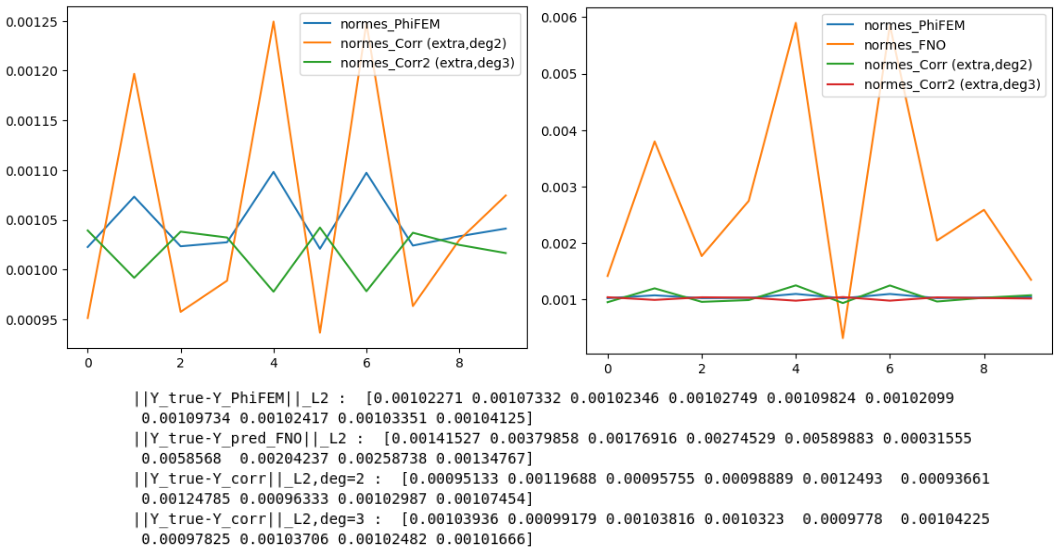
\includegraphics[width=0.9\linewidth]{comp_PhiFEM_FNO_Corr.png}
\end{minipage}

\subsection{Facteurs de division de l'erreur sur la solution analytique}

On considère encore la solution analytique trigonométrique suivante :
$$u_{ex}(x,y) = \frac{1}{\sin\left(k_1\frac{\pi}{2}\right)}\times\sin\left(k_1\frac{\pi}{2}\left(\frac{4}{\sqrt{2}}\right)^2\left((x-0.5)^2+(y-0.5)^2\right)\right)\times\cos\left(\frac{\pi}{2}\left(\frac{4}{\sqrt{2}}\right)^2\left((x-0.5)^2+(y-0.5)^2\right)\right)\,, $$ 

On cherche ici à déterminer les facteurs de division entre PhiFEM et la correction appliqué à la solution analytique. Voici les résultats obtenus :

\begin{minipage}{\linewidth}
	\centering
	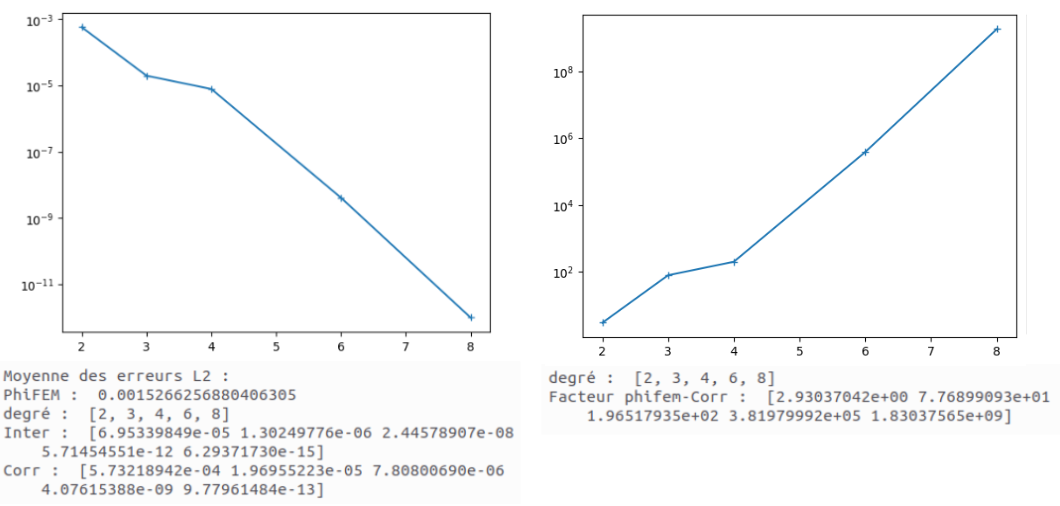
\includegraphics[width=0.8\linewidth]{test_degre.png}
\end{minipage}

\subsection{Pentes de convergence (interpolation et correction)}

On veut vérifier ici les pentes des droites de convergence sur la norme $L^2$ de la différence entre la solution exacte et son interpolation :
$$||u_{ex}-I_h u_{ex}||_{L^2(\Omega_h),rel}\sim h^{k+1}$$
Dans un second temps on cherche à déterminer numériquement la pente des droites de convergence sur la norme $L^2$ de la différence entre la solution exacte et la correction appliquée à son interpolation :
$$||u_{ex}-CI_h u_{ex}||_{L^2(\Omega_h),rel}\sim h^{?}$$

On traitera dans un premier temps le cas avec la solution analytique trigonométrique puis le cas où f est gaussienne où on prend comme solution de référence une solution sur-raffinée.

\subsubsection*{Solution analytique trigonométrique}

On considère encore la solution analytique trigonométrique suivante :
$$u_{ex}(x,y) = \frac{1}{\sin\left(k_1\frac{\pi}{2}\right)}\times\sin\left(k_1\frac{\pi}{2}\left(\frac{4}{\sqrt{2}}\right)^2\left((x-0.5)^2+(y-0.5)^2\right)\right)\times\cos\left(\frac{\pi}{2}\left(\frac{4}{\sqrt{2}}\right)^2\left((x-0.5)^2+(y-0.5)^2\right)\right)\,, $$ 

On considère la solution exacte $u_{ex}$ interpolé à un ordre assez élevé (de degré 8 par exemple). On interpole cette solution exacte (notre nouvelle level-set que l'on note $I_h u_{ex}$) dans $\mathbb{P}^k$ avec $k\in\{1,2,3\}$ et on fixe $C\in\mathbb{P}^1$.  

On obtient les résultats suivants :

\begin{minipage}{\linewidth}
	\centering
	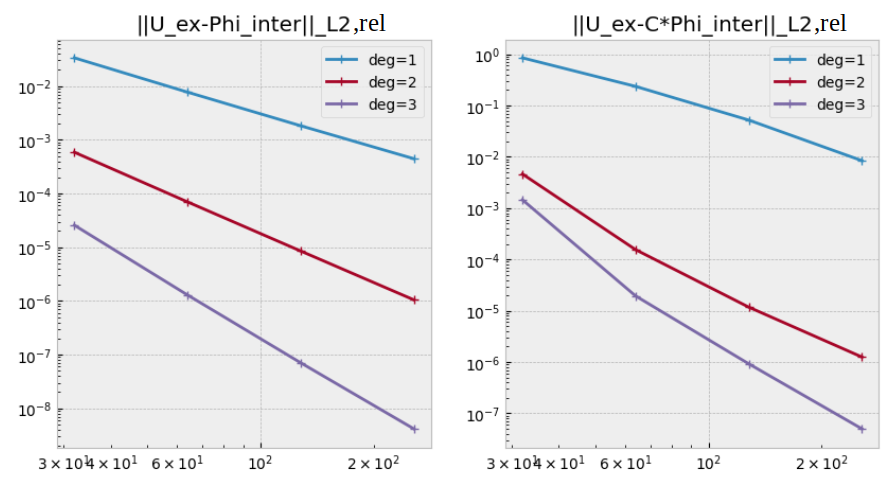
\includegraphics[width=0.6\linewidth]{cvg_sol_trigo.png}
\end{minipage}

On obtient
$$||u_{ex}-I_h u_{ex}||_{L^2(\Omega_h),rel}\sim h^{k+1}, \quad ||u_{ex}-CI_h u_{ex}||_{L^2(\Omega_h),rel}\sim h^{k+1}$$

\subsubsection*{f gaussienne}

On considère cette fois-ci $f$ gaussienne :
$$f(x,y) = \exp\left(-\frac{(x-\mu_0)^2 + (y-\mu_1)^2}{2\sigma^2}\right)\,, $$ 
avec $\sigma \sim \mathcal{U}([0.1,0.6])$ et $\mu_0, \mu_1 \sim \mathcal{U}([0.5-\sqrt{2}/4, 0.5+\sqrt{2}/4])$ à condition que $\phi(\mu_0, \mu_1) < -0.05$. \\

Dans un premier temps, on considère la solution de référence $u_{ex}$ comme étant une solution sur-raffinée obtenue par les EF standard (avec $h_{ex}\approx 0.006$ car $h_{ex}<<h_{FNO}$).  On interpole cette solution exacte (notre nouvelle level-set que l'on note $I_h u_{ex}$) dans $\mathbb{P}^k$ avec $k\in\{1,2,3\}$ et on fixe $C\in\mathbb{P}^1$.  


On obtient les résultats suivants :

\begin{minipage}{\linewidth}
	\centering
	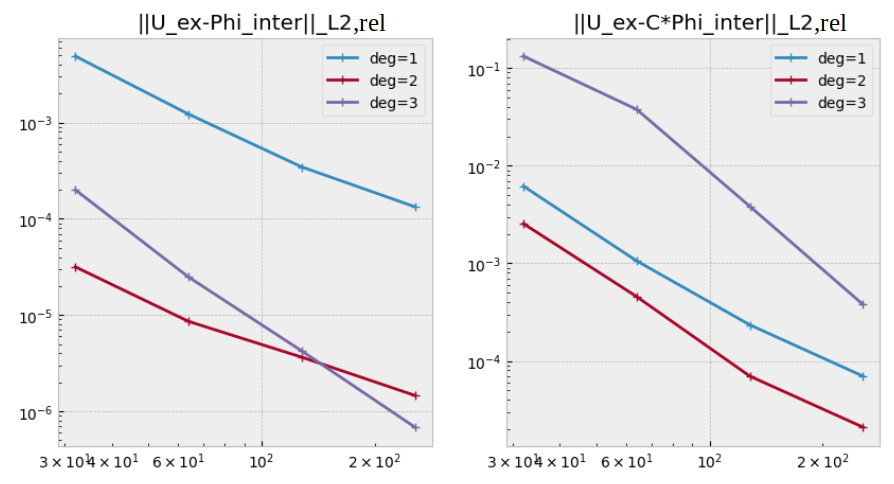
\includegraphics[width=0.6\linewidth]{cvg_f_gaussienne.png}
\end{minipage}

On obtient
$$||u_{ex}-I_h u_{ex}||_{L^2(\Omega_h),rel}\sim h^{k+1}, \quad ||u_{ex}-CI_h u_{ex}||_{L^2(\Omega_h),rel}\sim h^{k+1}$$

Cependant, il semblerait qu'il y ait un problème en $\mathbb{P}^3$ car l'erreur est plus grande qu'avec $k=1,2$. De plus la différence des erreurs en $×\mathbb{P}^1$ et en $\mathbb{P}^2$ est très petite. \\

Dans un second temps, on considère toujours la solution de référence $u_{ex}$ comme étant une solution sur-raffinée obtenue par les EF standard (avec $h\le 0.006$). On interpole cette fois-ci cette solution exacte (notre nouvelle level-set que l'on note $I_h u_{ex}$) dans $\mathbb{P}^{k+1}$ avec $k\in\{1,2,3\}$ et on prend $C\in\mathbb{P}^k$.  

On obtient les résultats suivants :

\begin{minipage}{\linewidth}
	\centering
	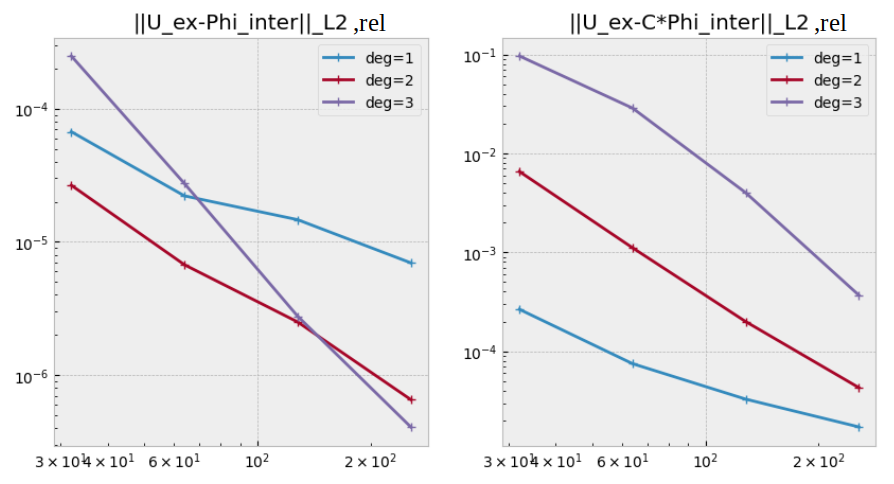
\includegraphics[width=0.6\linewidth]{cvg_f_gaussienne_2.png}
\end{minipage}

On obtient
$$||u_{ex}-I_h u_{ex}||_{L^2(\Omega_h),rel}\sim h^{k+1}, \quad ||u_{ex}-CI_h u_{ex}||_{L^2(\Omega_h),rel}\sim h^{k+1}$$

Cependant, il semblerait qu'il y ait un problème car l'erreur $\mathbb{P}^1$ est meilleure que l'erreur $\mathbb{P}^2$ qui elle-même est meilleure que l'erreur $\mathbb{P}^3$.


\subsection{Nouvelle idée FNO : Entraînement en $32\times 32 \; \mathbb{P}^2$}

On commence par générer $nb\_data$ données en $\mathbb{P}^2$ avec $nb\_vert=32$. Une première difficulté est de faire la conversion des résultats FEniCS en "image" Numpy. Ensuite, on entraîne le FNO avec ces données sur un certains nombres d'époques. On peut alors utiliser le FNO sur de nouvelles données (un échantillon test par exemple). On va ensuite corriger la sortie du FNO où une seconde difficulté est le passage de notre image Numpy (où chaque pixel représente la valeur de la solution en chacun des degré de liberté $\mathbb{P}^2$) à une Expression Fenics. Après la correction, on obtient la solution $\mathbb{P}^1$ (car $C\in\mathbb{P}^1$).

%\lstset{style=Python}

\textbf{Conversion FEniCS->Numpy : }

Cette conversion est effectuée lors de la génération des données. Le solveur PhiFEM nous fournit une expression FEniCS. Dans le cas $\mathbb{P}^1$, la fonction \textit{compute\_vertex\_values} de FEniCS nous permet de récupérer la valeur de la solution aux nœuds de notre maillage. En $\mathbb{P}^2$, c'est un peu plus compliqué, il faudra récupérer la valeur en chaque degré de liberté manuellement. Pour cela, on commence par récupérer les coordonnées de nos degrés de liberté en utilisant la fonction \textit{tabulate\_dof\_coordinates} de FEniCS. La complexité de cette méthode est que la numérotation FEniCS n'est pas la même que celle que l'on souhaiterais. C'est pour cela que l'on va devoir créer un mapping. Pour cela, on commence par récupérer le vecteur des coordonnées dont la première colonne contient $x$ et la deuxième contient $y$. On va rajouter une colonne contenant une nouvelle indexation de nos coordonnée. Puis, on trie cette matrice selon les ordonnées puis selon les abscisses. On obtient alors les coordonnées triées de bas en haut et de gauche à droite. La colonne contenant les indices est alors notre mapping. On peut alors ordonner l'expression et on obtient le tableau Numpy.

\textbf{Conversion Numpy->FEniCS : }

Cette conversion est utilisée pour convertir notre sortie de FNO en une fonction FEniCS pour la Correction. De la même manière, que pour la conversion dans le sens inverse, on crée un mapping qui nous permet d'associer chaque degré de liberté FEniCS aux valeurs Numpy.



\subsubsection{Solution analytique trigonométrique}

On considère encore la solution analytique trigonométrique suivante :
$$u_{ex}(x,y) = \frac{1}{\sin\left(k_1\frac{\pi}{2}\right)}\times\sin\left(k_1\frac{\pi}{2}\left(\frac{4}{\sqrt{2}}\right)^2\left((x-0.5)^2+(y-0.5)^2\right)\right)\times\cos\left(\frac{\pi}{2}\left(\frac{4}{\sqrt{2}}\right)^2\left((x-0.5)^2+(y-0.5)^2\right)\right)\,, $$ 

\newpage
Après entraînement sur 4000 époques voici les misfits obtenus : 

\begin{minipage}{\linewidth}
	\centering
	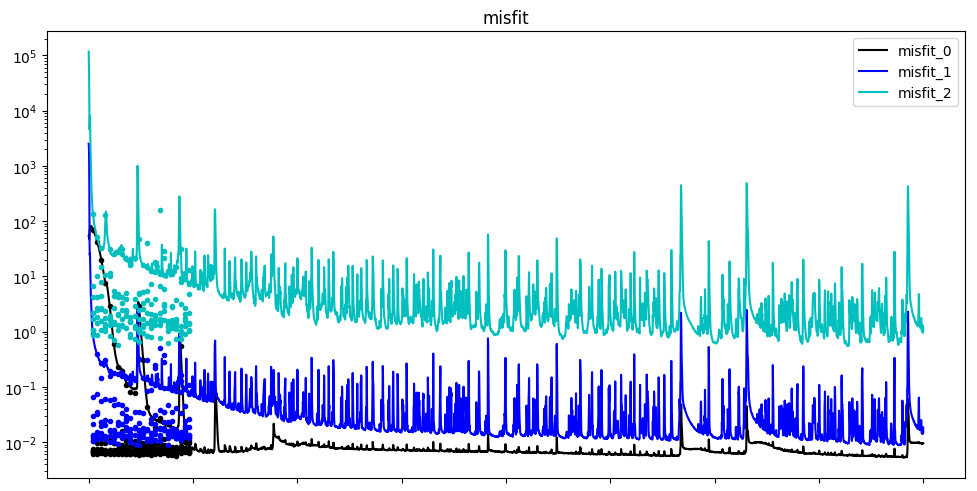
\includegraphics[width=0.7\linewidth]{FNO_trigo/misfits_sol_trigo.png}
\end{minipage}

\fbox{A RELANCER EN UNE TRAITE !}


\textbf{Échantillon de validation :}

On commence par calculer les erreurs en norme $L^2$ sur l'échantillon de validation. On considérera des "sous-modèle" qui seront sauvegarder toutes les 500 époques. A gauche, on a les erreurs sur l'échantillon de validations toutes les 1000 époques. A droite, il y a la moyenne, l'écart-type, le minimum et le maximum de l'erreur sur l'échantillon de validation pour chacun des sous-modèle (500,1000,1500,2000,2500,3000,3500 et 4000).

\begin{minipage}{0.48\linewidth}
	\centering
	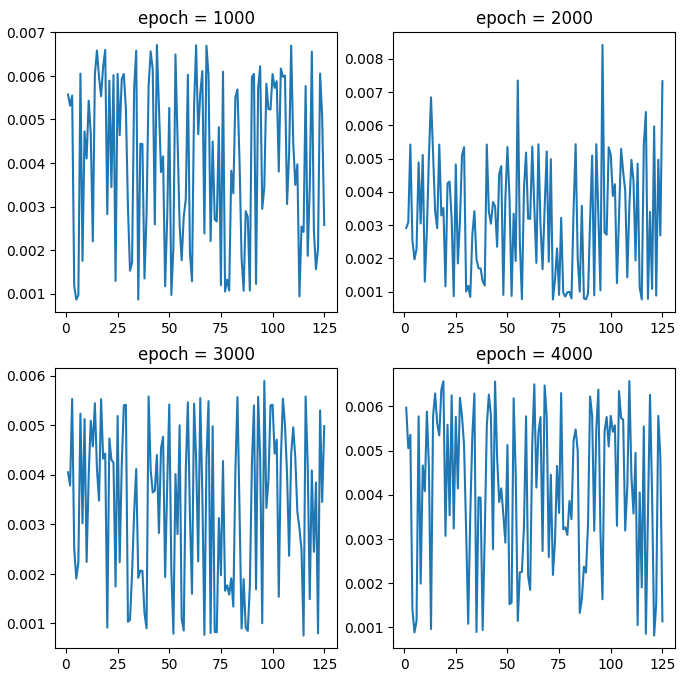
\includegraphics[width=0.8\linewidth]{FNO_trigo/erreur_val_sol_trigo.png}
\end{minipage}
\begin{minipage}{0.48\linewidth}
	\centering
	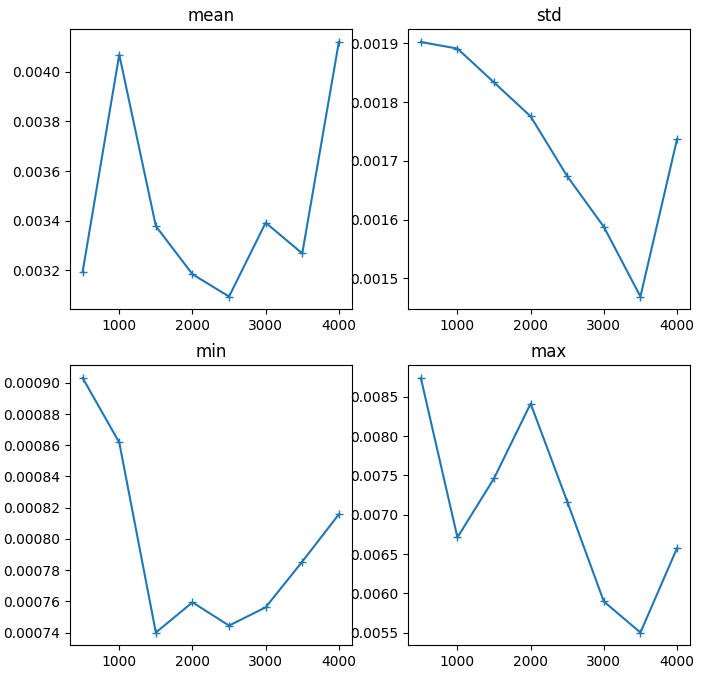
\includegraphics[width=0.8\linewidth]{FNO_trigo/infos_val_sol_trigo.png}
\end{minipage}

On réalise également un histogramme pour chacun des sous-modèles : 

\begin{minipage}{\linewidth}
	\centering
	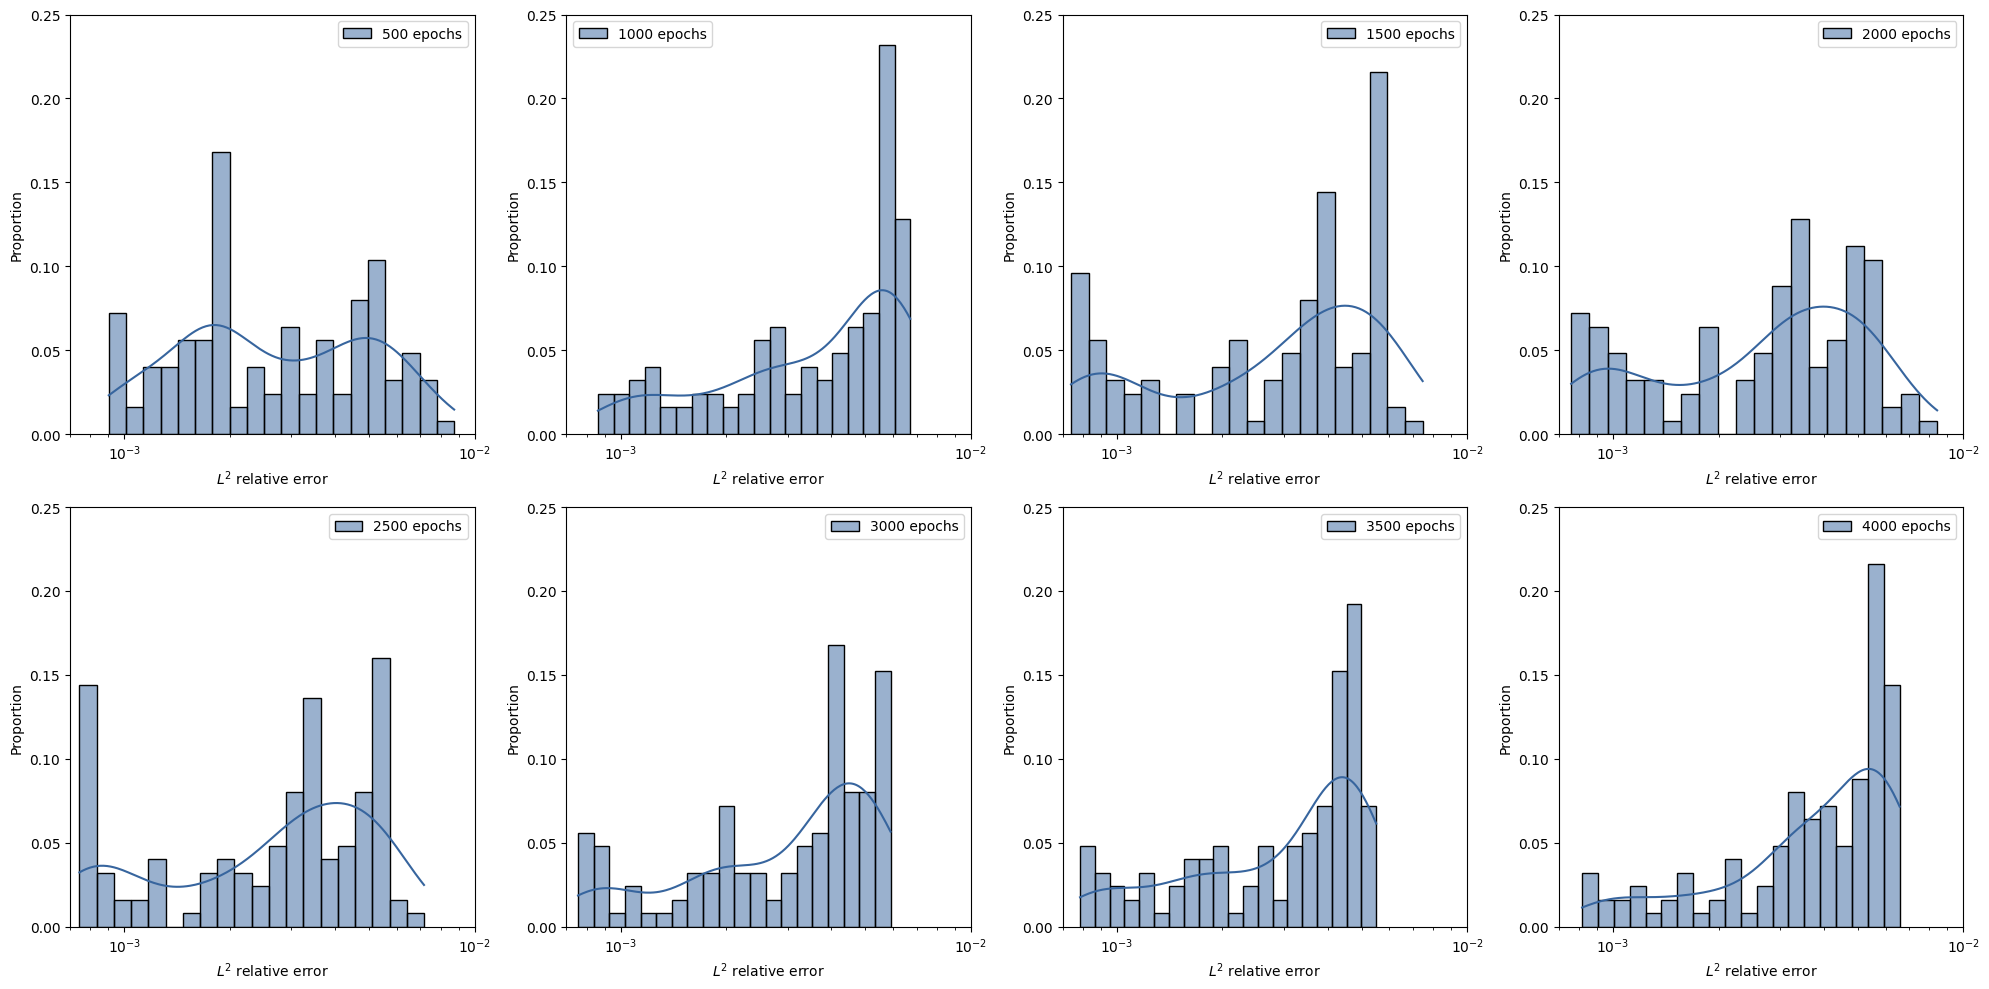
\includegraphics[width=0.8\linewidth]{FNO_trigo/histogram_val_sol_trigo.png}
\end{minipage}

\newpage

\textbf{Échantillon test :}
On s'intéresse exactement aux même résultats mais cette fois-ci sur un nouvel échantillon (un échantillon test de taille 100) :

\begin{minipage}{0.48\linewidth}
	\centering
	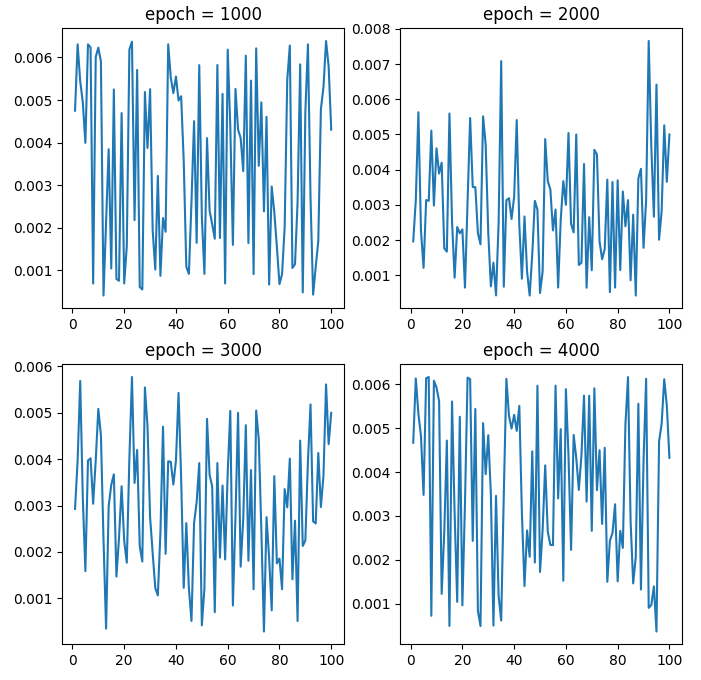
\includegraphics[width=0.8\linewidth]{FNO_trigo/erreur_test_sol_trigo.png}
\end{minipage}
\begin{minipage}{0.48\linewidth}
	\centering
	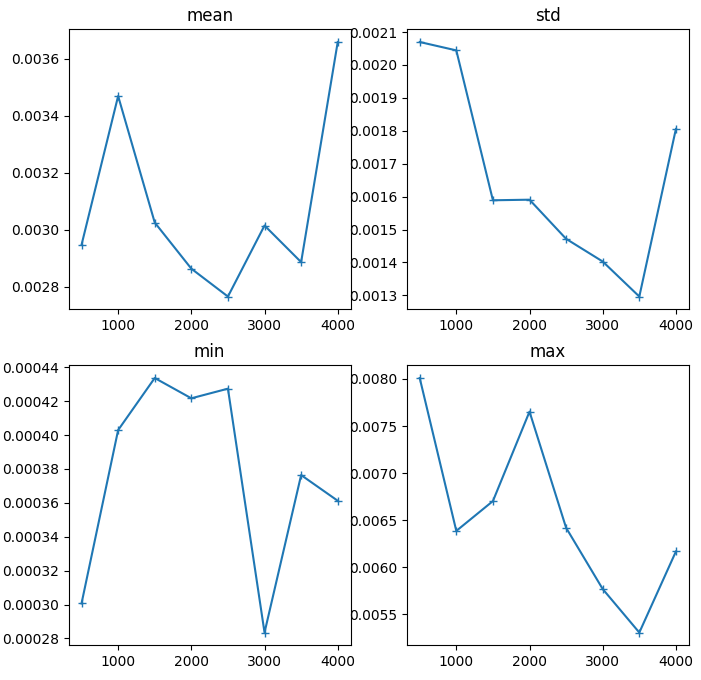
\includegraphics[width=0.8\linewidth]{FNO_trigo/infos_test_sol_trigo.png}
\end{minipage}

\begin{minipage}{\linewidth}
	\centering
	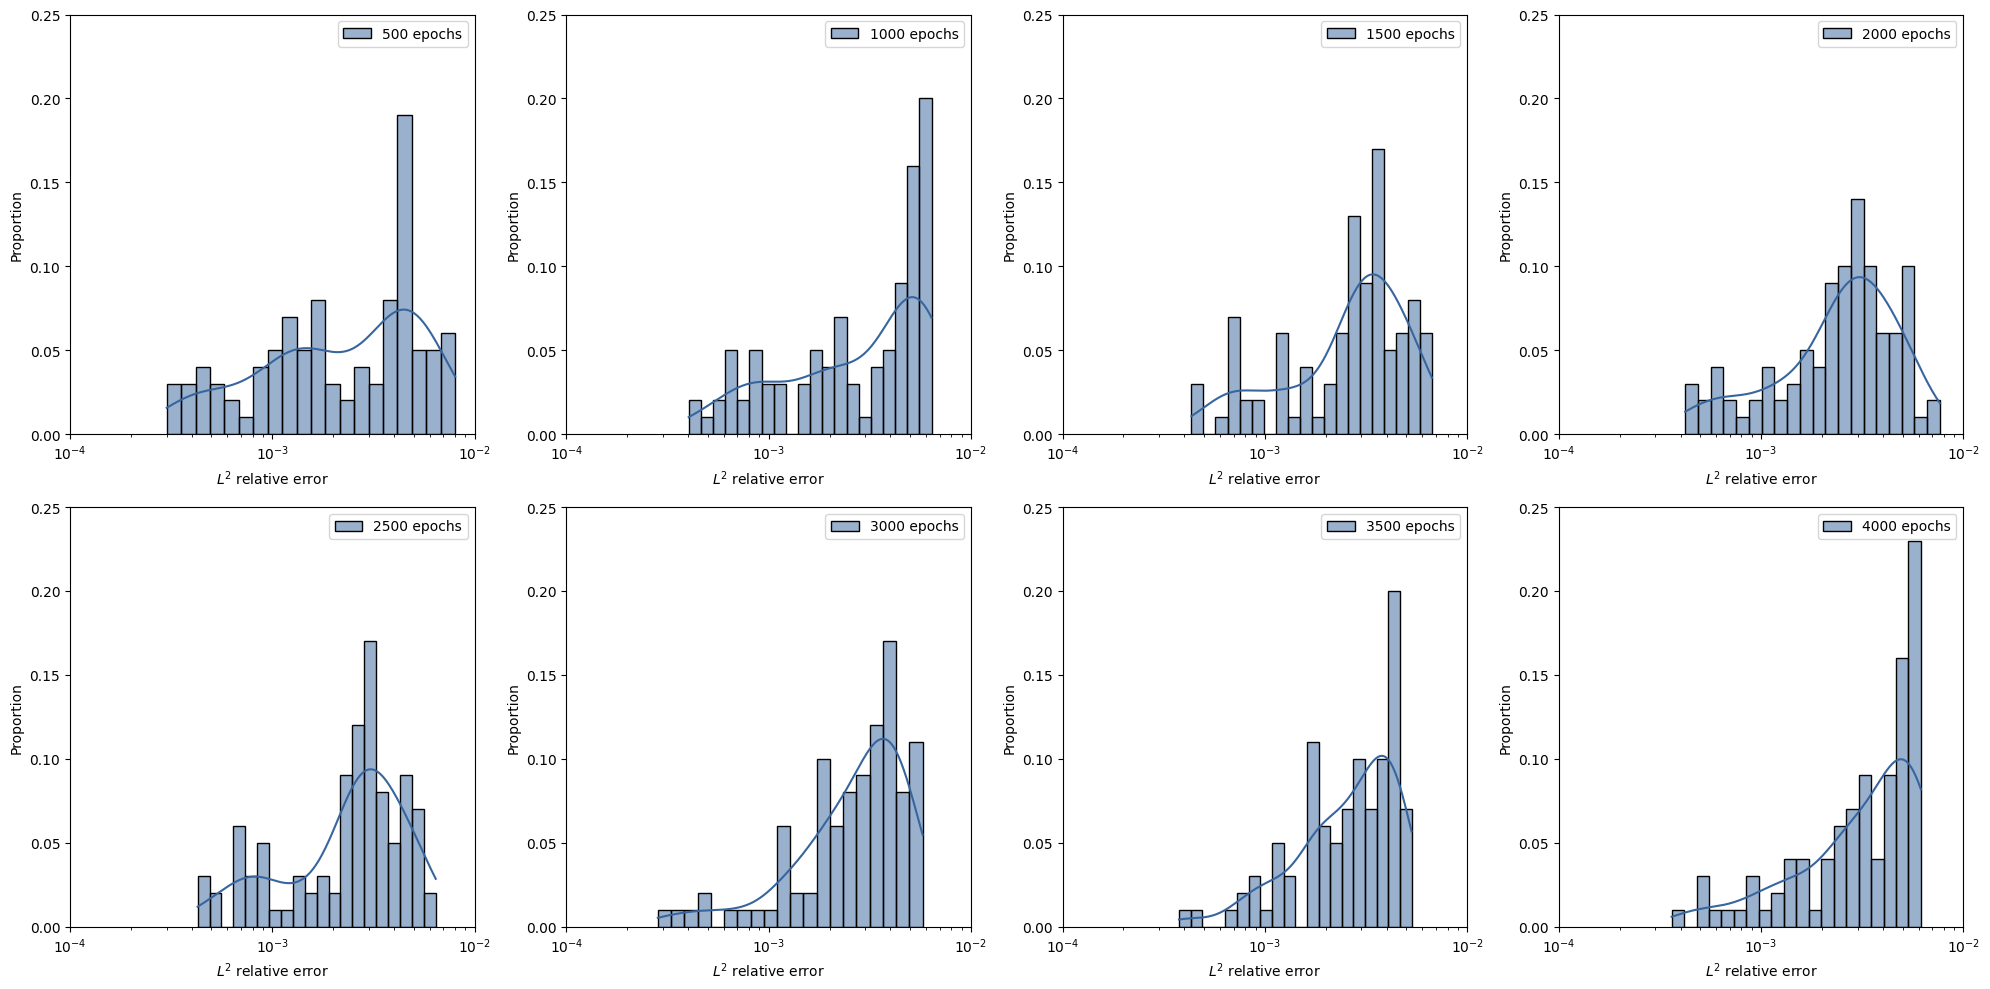
\includegraphics[width=0.8\linewidth]{FNO_trigo/histogram_test_sol_trigo.png}
\end{minipage}

\textbf{Résultat après correction : }

On cherche à tester la correction sur la sortie du FNO. Voici un exemple de résultat :

\begin{minipage}{\linewidth}
	\centering
	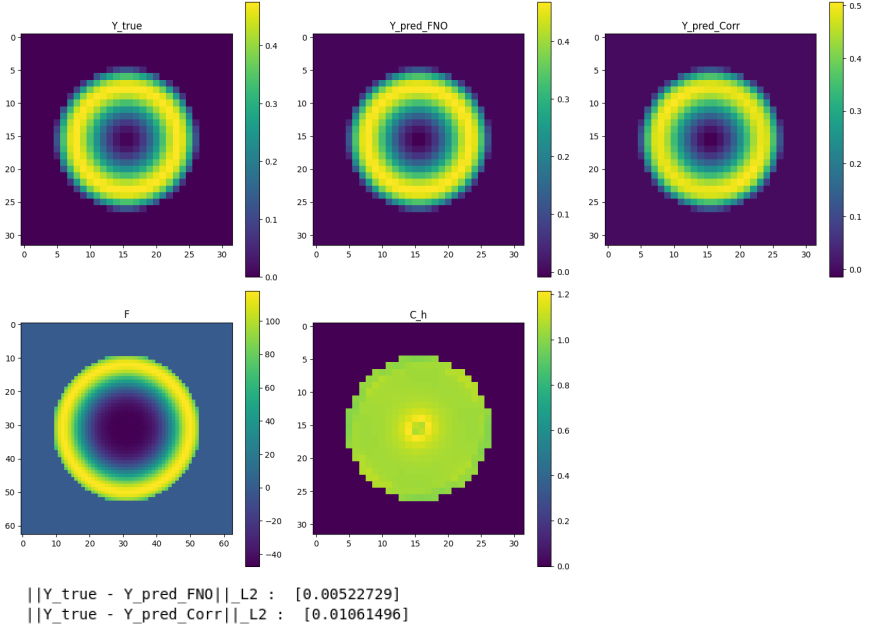
\includegraphics[width=0.68\linewidth]{FNO_trigo/resultat_sol_trigo.png}
\end{minipage}


On pense que les données précédentes ne varient pas assez et qu'elles sont donc trop facile à apprendre par le FNO. En effet, au bout de déjà 500 époques les erreurs semblent très bonnes. Ainsi la correction a du mal à être meilleure que la sortie du FNO. On va donc considérer un nouveau problème plus compliqué. On considère toujours le problème de poisson avec condition de Dirichlet homogène. On prend $f$ gaussienne et notre solution de référence sera une solution sur-raffinée obtenue par les éléments finis standard.

\subsubsection{f gaussienne}

On considère cette fois-ci $f$ gaussienne :
$$f(x,y) = \exp\left(-\frac{(x-\mu_0)^2 + (y-\mu_1)^2}{2\sigma^2}\right)\,, $$ 
avec $\sigma \sim \mathcal{U}([0.1,0.6])$ et $\mu_0, \mu_1 \sim \mathcal{U}([0.5-\sqrt{2}/4, 0.5+\sqrt{2}/4])$ à condition que $\phi(\mu_0, \mu_1) < -0.05$. \\

Après entraînement sur 4000 époques voici les misfits obtenus : 

\begin{minipage}{\linewidth}
	\centering
	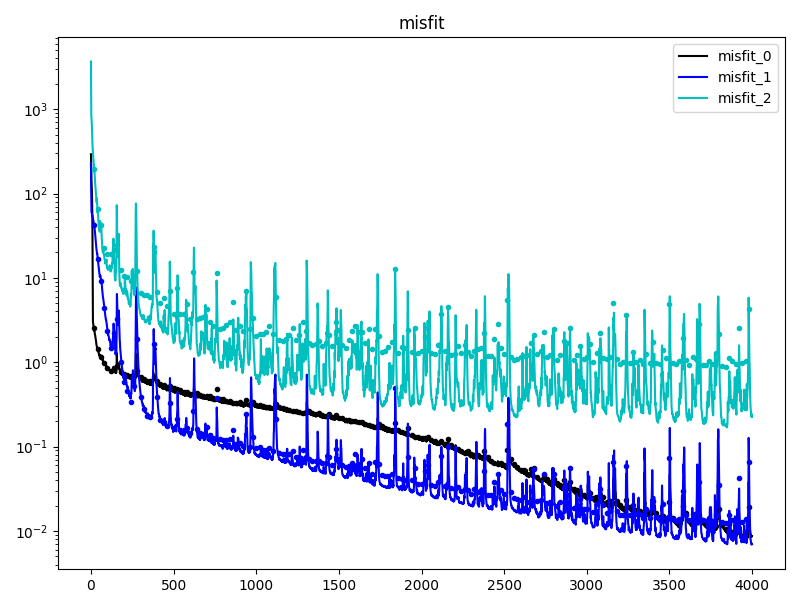
\includegraphics[width=0.6\linewidth]{FNO_gaussienne/misfits_f_gaussienne.png}
\end{minipage}

\textbf{Échantillon de validation :}

On commence par calculer les erreurs en norme $L^2$ sur l'échantillon de validation. On considérera des "sous-modèle" qui seront sauvegarder toutes les 500 époques. Voici les erreurs obtenus sur l'échantillon de validation pour chacun des sous-modèles :

\begin{minipage}{\linewidth}
	\centering
	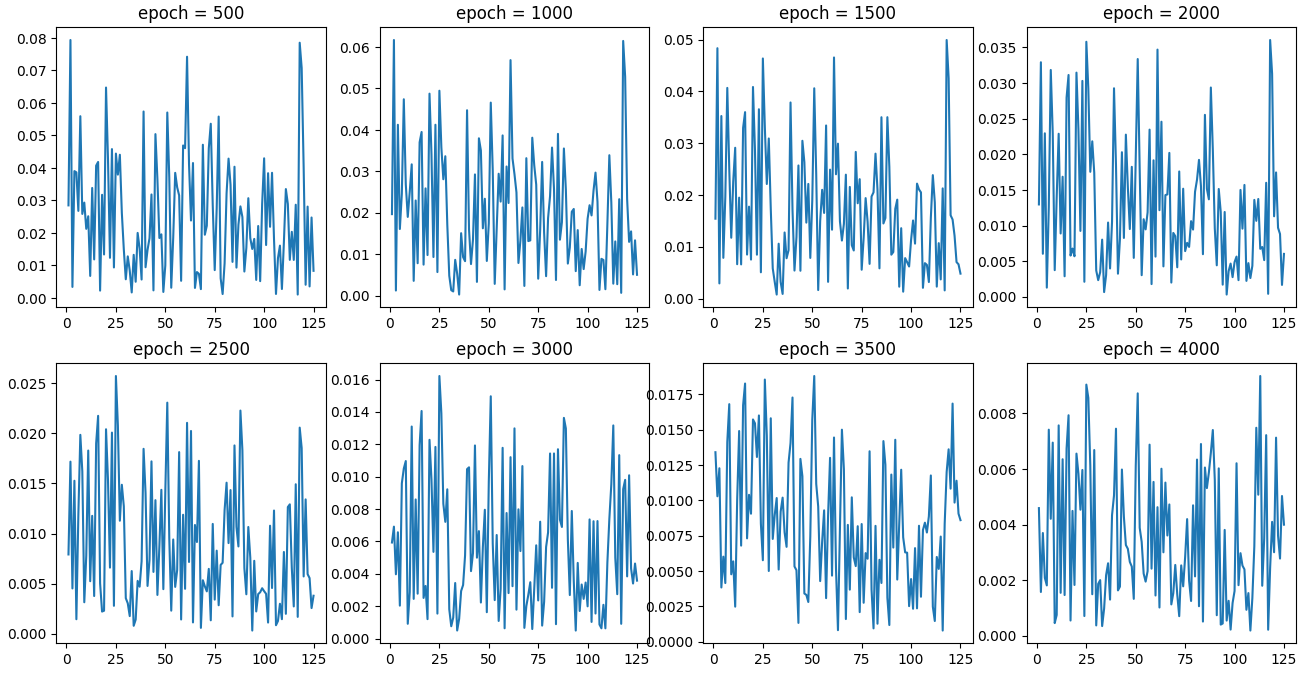
\includegraphics[width=0.9\linewidth]{FNO_gaussienne/erreur_val_f_gaussienne.png}
\end{minipage}

Voici la moyenne, l'écart-type, le minimum et le maximum de l'erreur sur l'échantillon de validation pour chacun des sous-modèle (500,1000,1500,2000,2500,3000,3500 et 4000) :

\begin{minipage}{\linewidth}
	\centering
	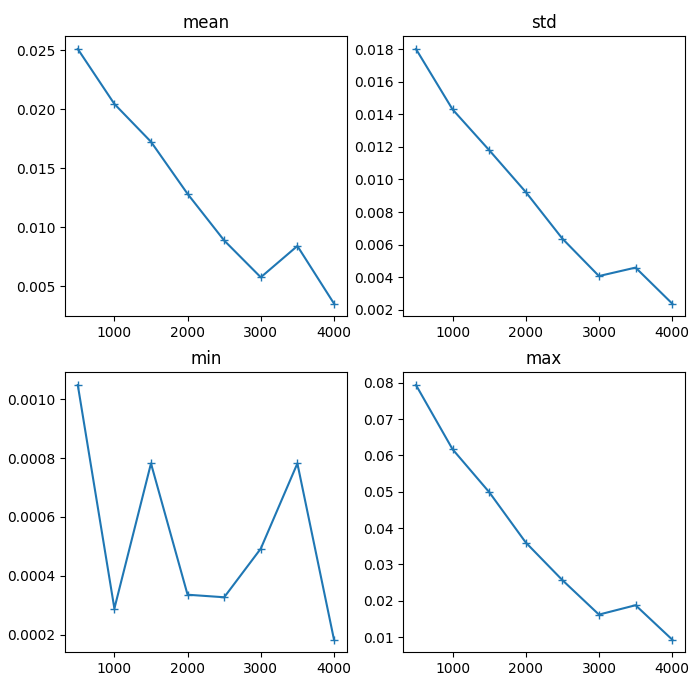
\includegraphics[width=0.4\linewidth]{FNO_gaussienne/infos_val_f_gaussienne.png}
\end{minipage}

On réalise également un histogramme pour chacun des sous-modèles : 

\begin{minipage}{\linewidth}
	\centering
	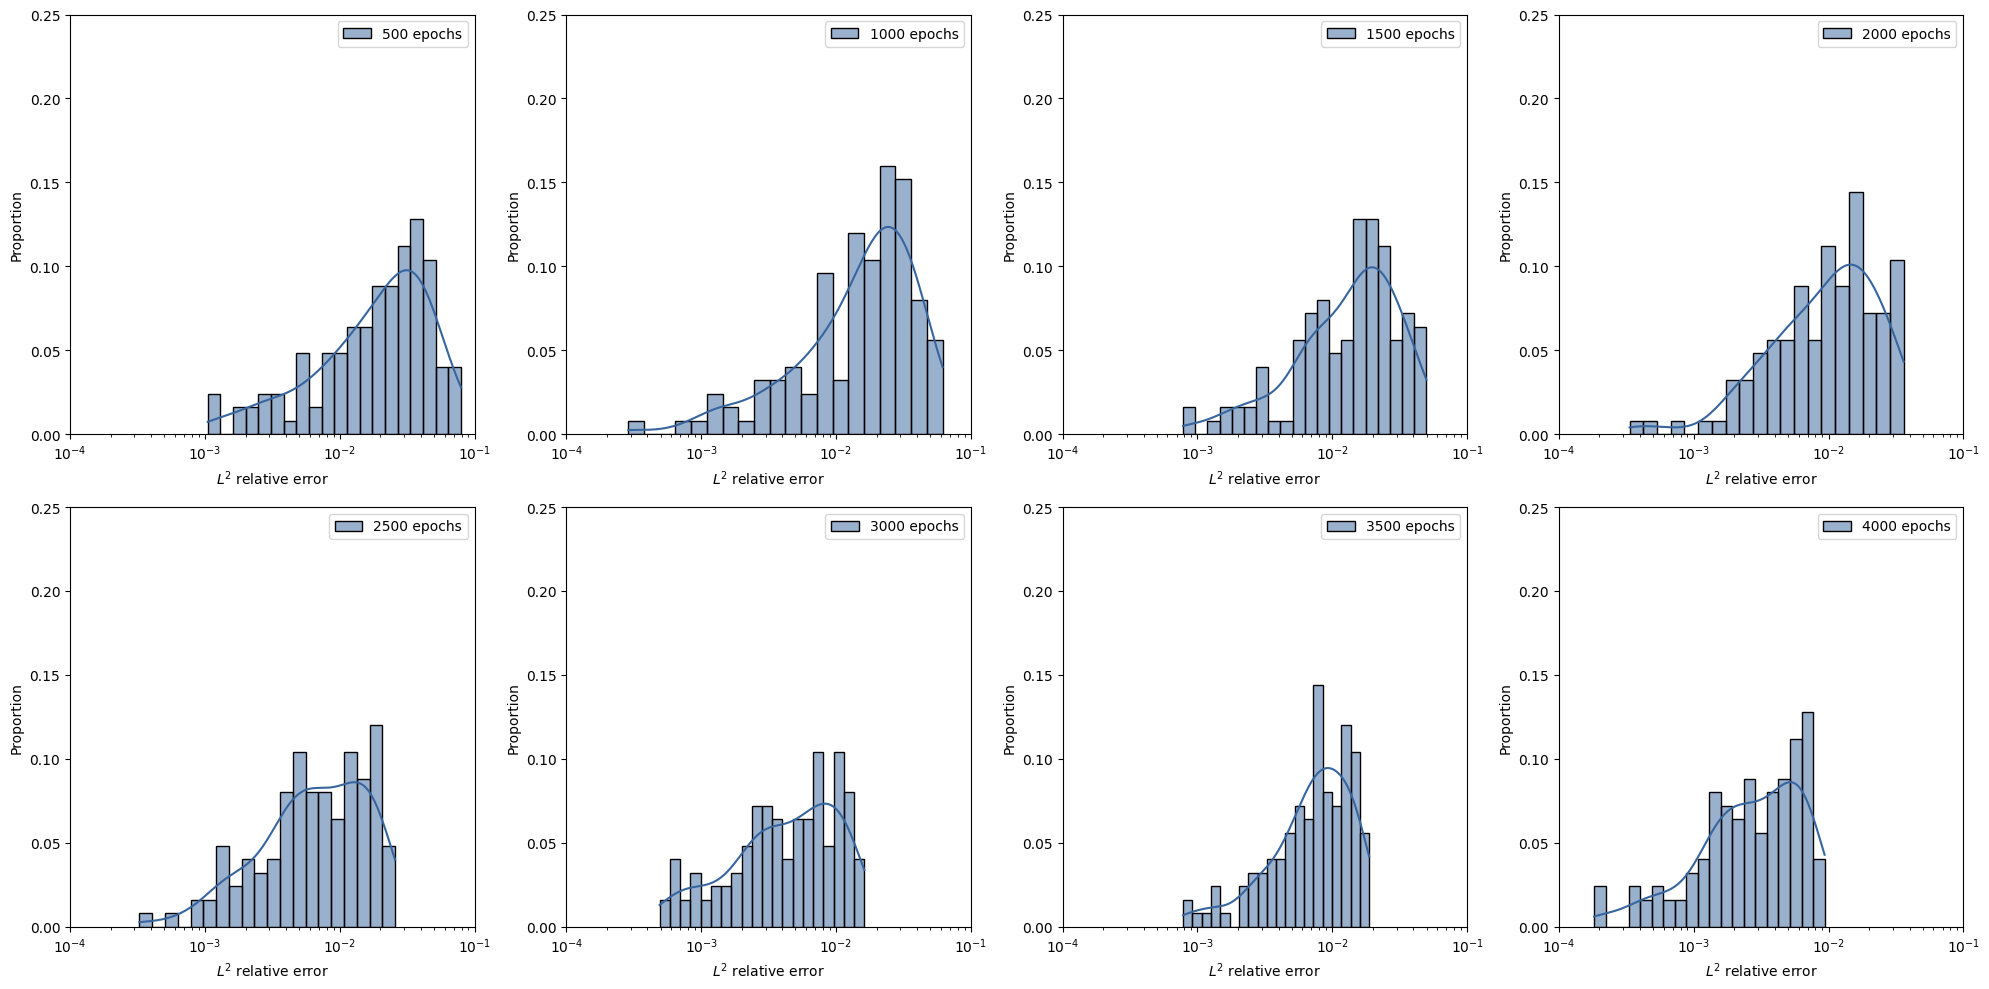
\includegraphics[width=0.8\linewidth]{FNO_gaussienne/histogram_val_f_gaussienne.png}
\end{minipage}

\textbf{Échantillon test :}
On s'intéresse exactement aux même résultats mais cette fois-ci sur un nouvel échantillon (un échantillon test de taille 100) :

\begin{minipage}{\linewidth}
	\centering
	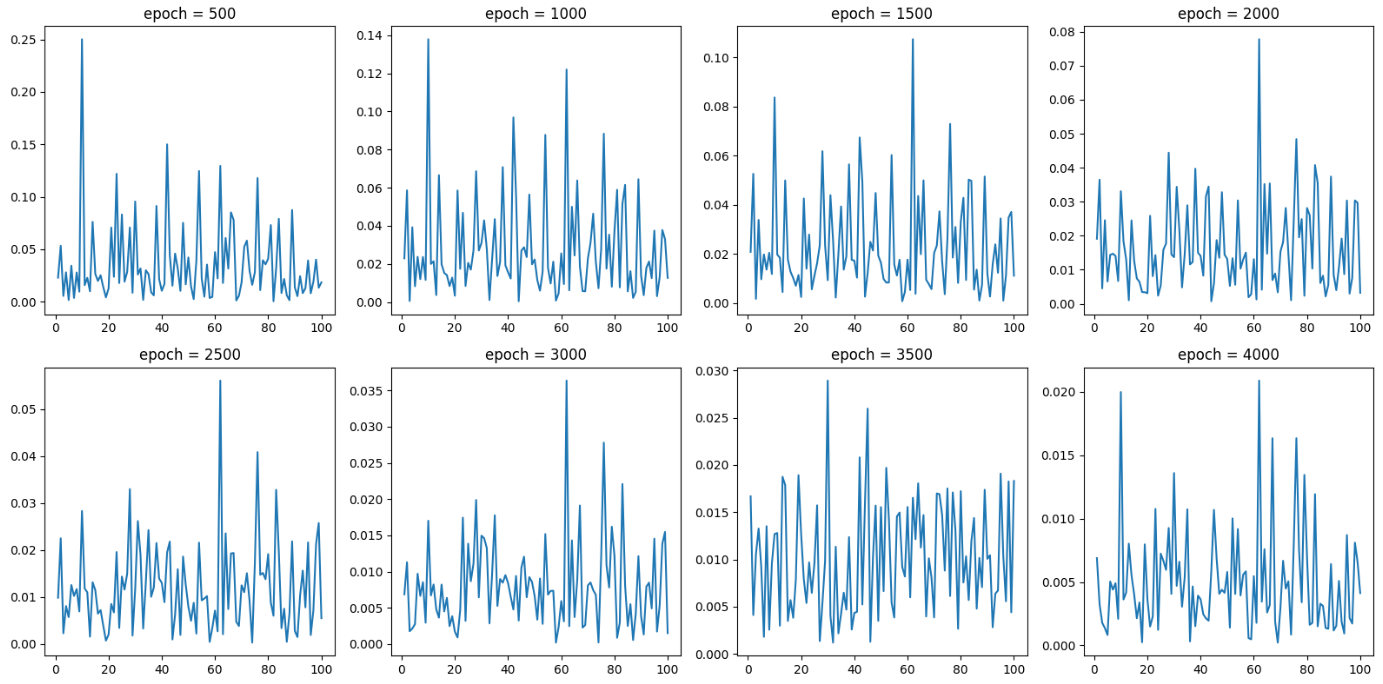
\includegraphics[width=0.9\linewidth]{FNO_gaussienne/erreur_test_f_gaussienne.png}
\end{minipage}

\begin{minipage}{\linewidth}
	\centering
	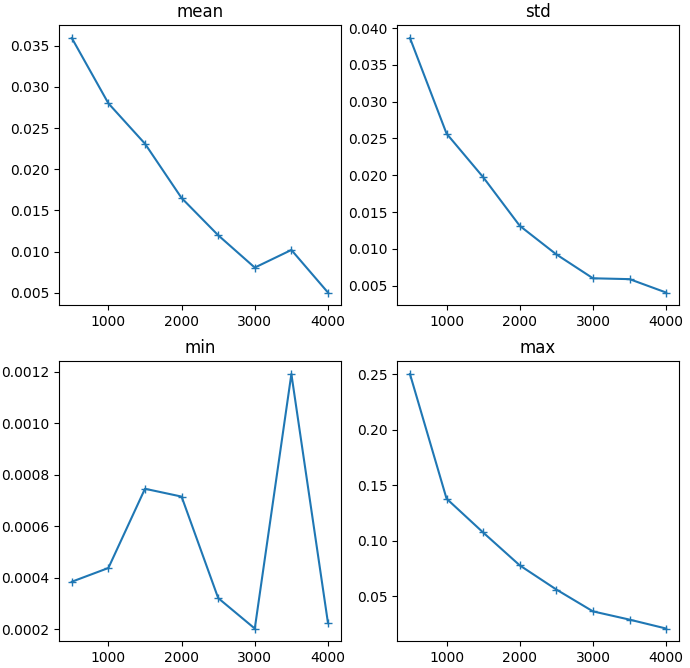
\includegraphics[width=0.45\linewidth]{FNO_gaussienne/infos_test_f_gaussienne.png}
\end{minipage}

\begin{minipage}{\linewidth}
	\centering
	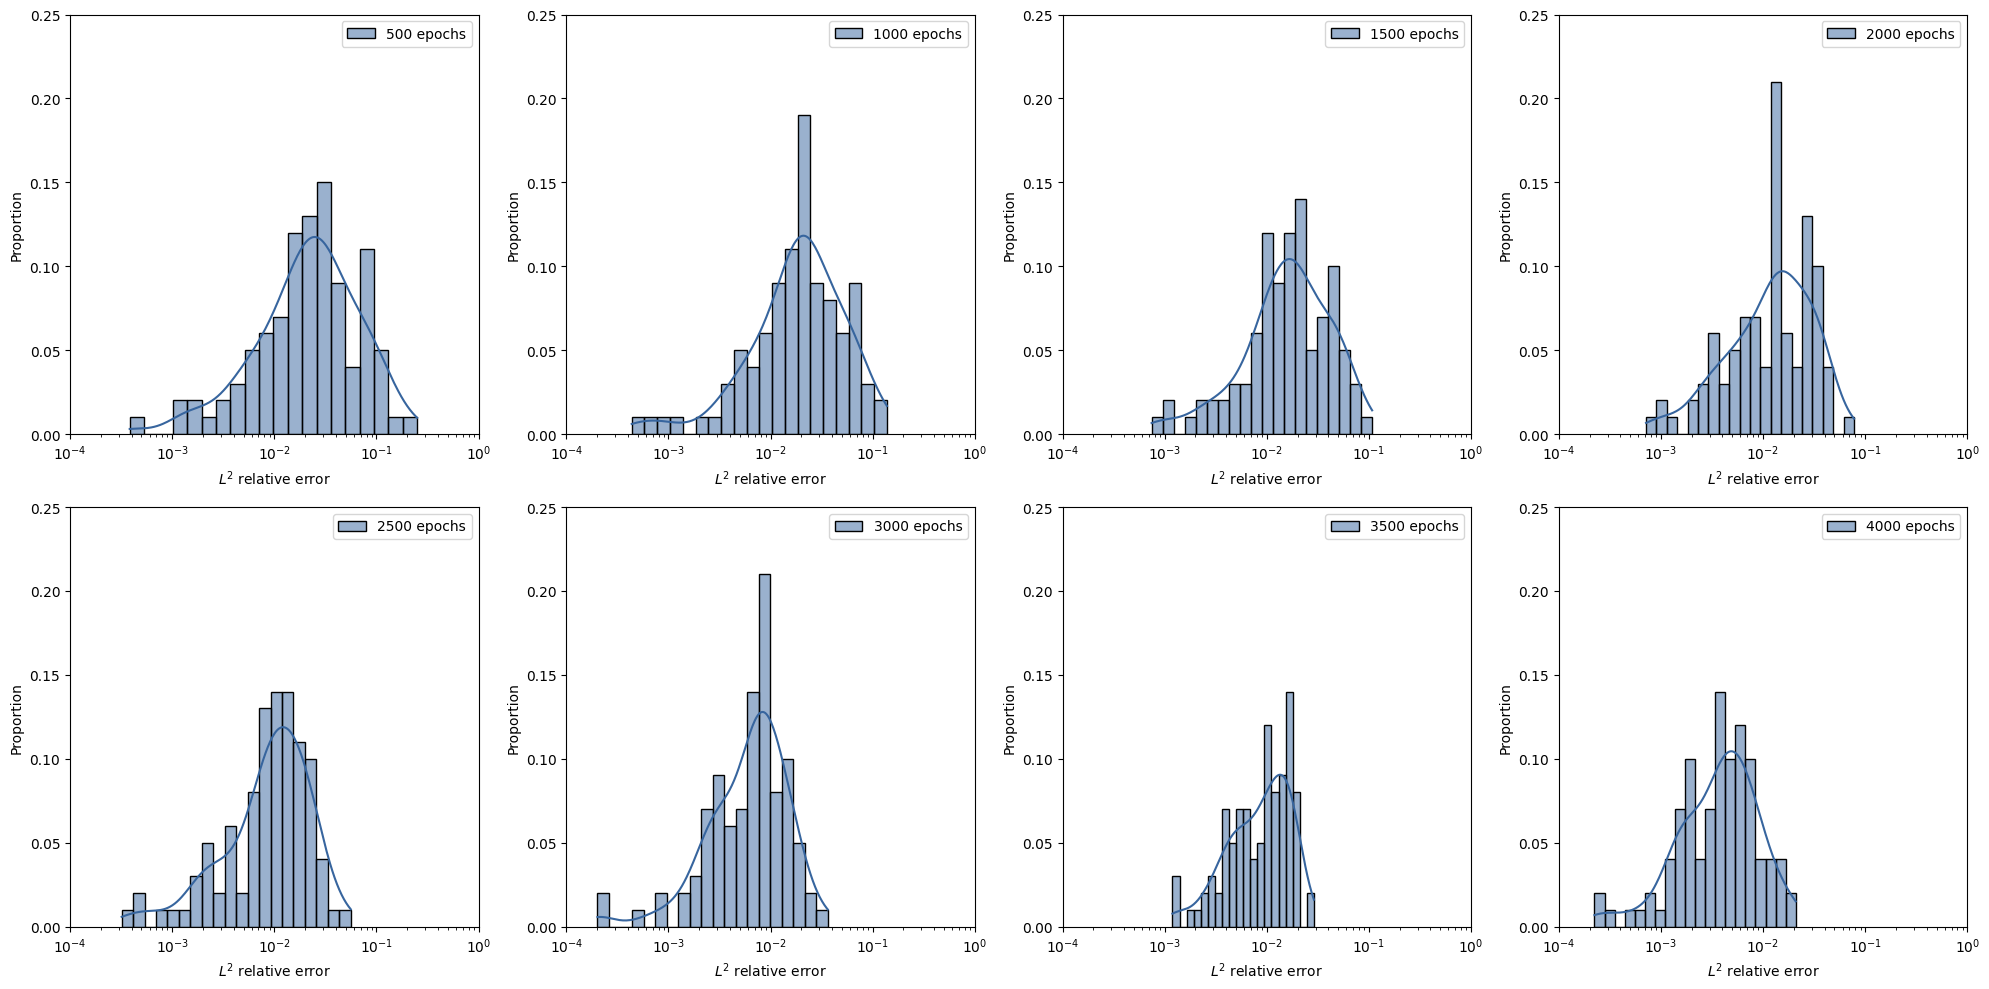
\includegraphics[width=0.8\linewidth]{FNO_gaussienne/histogram_test_f_gaussienne.png}
\end{minipage}

\textbf{Résultat après correction : }

On cherche à tester la correction sur la sortie du FNO. 

\begin{minipage}{\linewidth}
	\centering
	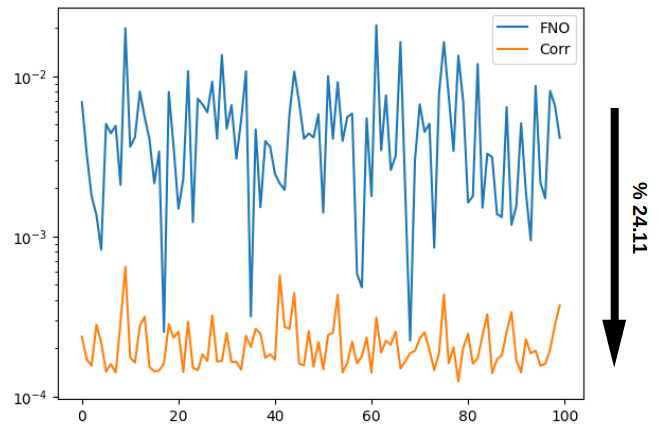
\includegraphics[width=0.68\linewidth]{FNO_gaussienne/resultats_test.png}
\end{minipage}
	
	\newpage
	\section{Semaine 8 : 27/03/2023 - 31/03/2023}
\graphicspath{{semaines/semaine_8/images/}}

\begin{abstract}
	L'idée principale de la semaine et de tester de rehausser la solution. Deux méthodes ont été proposées : rehausser par une constante $m$ (proposée par Emmanuel) ou rehausser par la level-set initial $\phi$ (proposée par Michel).
	
	J'ai également essayé de faire des boxplots pour comparer FEM standard, $\phi$-FEM, FNO et FNO+Corr (pour différents nombres d'époques).
\end{abstract}

\subsection{Rehaussement}

On considère toujours le problème initial

$$\left\{\begin{aligned}
	&-\Delta u=f \quad &&\Omega \\
	&u=0 \quad &&\Gamma
\end{aligned}\right.$$

On prend encore la solution analytique trigonométrique suivante :
$$u_{ex}(x,y) = \frac{1}{\sin\left(k_1\frac{\pi}{2}\right)}\times\sin\left(k_1\frac{\pi}{2}\left(\frac{4}{\sqrt{2}}\right)^2\left((x-0.5)^2+(y-0.5)^2\right)\right)\times\cos\left(\frac{\pi}{2}\left(\frac{4}{\sqrt{2}}\right)^2\left((x-0.5)^2+(y-0.5)^2\right)\right)$$ 

avec $k_1 \sim \mathcal{U}([0.1,1])$.

\subsubsection*{Par une constante}

On considère la solution rehaussée par $m$ :
$$\tilde{\phi}=u+m$$

avec $m$ une constante.

Voici la solution pour $k_1=0.5$ et $m=1$ (à gauche la solution $u$, à droite la solution rehaussée $\tilde{\phi}$) :

\begin{minipage}{\linewidth}
	\centering
	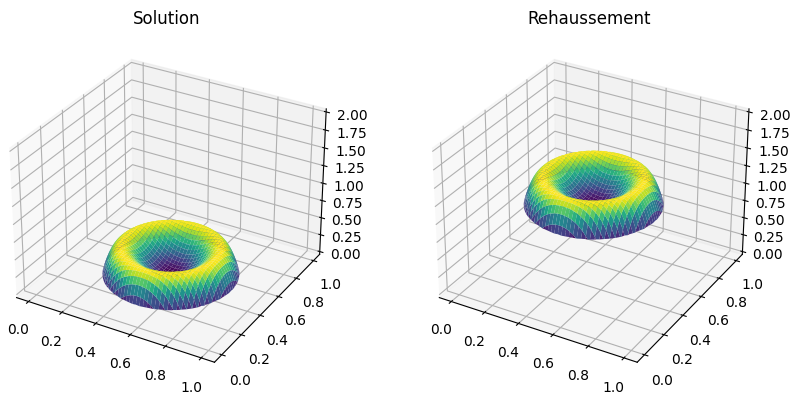
\includegraphics[width=0.5\linewidth]{rehaussement_cste.png}
\end{minipage}

On réécrit alors le problème par

$$\left\{\begin{aligned}
	&-\Delta (\tilde{\phi}-m)=f \quad &&\Omega \\
	&\tilde{\phi}=m \quad &&\Gamma
\end{aligned}\right.$$

Donc

$$\left\{\begin{aligned}
	&-\Delta \tilde{\phi}=f \quad &&\Omega \\
	&\tilde{\phi}=m \quad &&\Gamma
\end{aligned}\right.$$

On veut appliquer la correction, on pose alors $\tilde{u}=\tilde{\phi}C$
avec $\tilde{\phi}$ la level-set.

On a 

$$\left\{\begin{aligned}
	&-\Delta \tilde{u}=f \quad &&\Omega \\
	&\tilde{u}=m \quad &&\Gamma
\end{aligned}\right.$$

On se ramène alors à la correction du problème initial en posant
$$u_c = \tilde{\phi}C-m$$

On prend nb\_data=10. On cherche à comparer la moyenne des erreurs PhiFEM sur les nb\_data données avec la Correction pour différents degré d'intepolation de la levelset et avec la Correction par rehaussement pour différents degré d'interpolation et différents $m$. Voici les résultats obtenus :

\begin{minipage}{\linewidth}
	\centering
	\includegraphics[width=0.8\linewidth]{resultats_cste.png}
\end{minipage}

Et les facteurs obtenus :

\begin{minipage}{\linewidth}
	\centering
	\includegraphics[width=0.8\linewidth]{facteurs_cste.png}
\end{minipage}

\newpage
\subsubsection*{Par la level-set $\phi$}

On considère la solution rehaussée par une constante multipliée par $\phi$ :
$$\tilde{\phi}=u-\alpha\phi$$

avec $\alpha$ une constante positive.

Voici la solution pour $k_1=0.5$ et $\alpha=2$ (à gauche la solution $u$, à droite la solution rehaussée $\tilde{\phi}$) :

\begin{minipage}{\linewidth}
	\centering
	\includegraphics[width=0.5\linewidth]{rehaussement_phi.png}
\end{minipage}

On réécrit alors le problème par

$$\left\{\begin{aligned}
	&-\Delta (\tilde{\phi}+\alpha\phi)=f \quad &&\Omega \\
	&\tilde{\phi}=0 \quad &&\Gamma
\end{aligned}\right.$$

Donc

$$\left\{\begin{aligned}
	&-\Delta \tilde{\phi}=\tilde{f} \quad &&\Omega \\
	&\tilde{\phi}=0 \quad &&\Gamma
\end{aligned}\right.$$

avec $\tilde{f}=f+\alpha\Delta\phi$.

On veut appliquer la correction, on pose alors $\tilde{u}=\tilde{\phi}C$
avec $\tilde{\phi}$ la level-set.

On a 

$$\left\{\begin{aligned}
	&-\Delta \tilde{u}=\tilde{f} \quad &&\Omega \\
	&\tilde{u}=0 \quad &&\Gamma
\end{aligned}\right.$$

On se ramène alors à la correction du problème initial en posant
$$u_c = \tilde{\phi}C+\alpha\phi$$

Voici les résultats obtenus :

\begin{minipage}{\linewidth}
	\centering
	\includegraphics[width=0.7\linewidth]{resultats_phi.png}
\end{minipage}

\subsection{Résultats avec le FNO}

On considère cette fois-ci $f$ gaussienne :
$$f(x,y) = \exp\left(-\frac{(x-\mu_0)^2 + (y-\mu_1)^2}{2\sigma^2}\right)\,, $$ 
avec $\sigma \sim \mathcal{U}([0.1,0.6])$ et $\mu_0, \mu_1 \sim \mathcal{U}([0.5-\sqrt{2}/4, 0.5+\sqrt{2}/4])$ à condition que $\phi(\mu_0, \mu_1) < -0.05$. \\

Dans un premier temps, on considère la solution de référence $u_{ref}$ comme étant une solution sur-raffinée $\mathbb{P}^1$ obtenue par les EF standard (avec $h_{ref}\approx 0.006$ car $h_{ref}<<h_{FNO}$). 

On cherche à afficher des boxplots (boite à moustache) sur les erreurs en norme $L^2$ pour FEM standard, PhiFEM, le FNO et le FNO corrigé pour différents nombres d'époques. On prendra un nouvel échantillon test avec nb\_data=100. 

On va donc comparer
$$||u_{ref}-u_{FEM}||_{L^2,rel}, \quad ||u_{ref}-u_{\phi-FEM}||_{L^2,rel}, \quad ||u_{ref}-u_{FNO}||_{L^2,rel}, \quad ||u_{ref}-Cu_{FNO}||_{L^2,rel}$$

où $u_{FEM}$ est la solution $\mathbb{P}^1$ obtenue par la méthode des éléments finis standard avec une taille de maillage comparable à celle utilisée pour le FNO, $u_{\phi-FEM}$ est la solution $\mathbb{P}^1$ obtenue par $\phi$-FEM, $u_{FNO}$ est la solution $\mathbb{P}^2$ obtenue par le FNO et $C$ est la correction $\mathbb{P}^1$ obtenue en prenant comme level-set $u_{FNO}$.

Voici les résultats obtenus :

\begin{minipage}{\linewidth}
	\centering
	\includegraphics[width=0.7\linewidth]{boxplots.png}
\end{minipage}

\conclusion{Les résultats pour le rehaussement n'ont pas l'air bon : il faudra en parler la semaine prochaine avec Emmanuel et Michel.
	
Pour la partie avec le FNO, la semaine prochaine il faudrait comparer les temps d'exécution entre PhiFEM et FNO+Corr (ratio temps/erreur ou erreur/temps).}
	
	\newpage
	\section{Semaine 9 : 03/04/2023 - 07/04/2023}
\graphicspath{{semaines/semaine_9/images/}}

\begin{abstract}
	Après les résultats obtenus avec le FNO, on va essayer de comparer les temps d'exécution et les erreurs obtenus pour FEM, Phi-FEM, le FNO et le FNO+corr à différentes époques.
	
	Après discussion avec Emmanuel, on va considérer une level-set du type $\tilde{\phi}=u_{ex}+\epsilon*P$. On va tester le rehaussement avec FEM puis avec PhiFEM pour différents $m$ sur cette solution perturbée.
	
	(Vendredi est férié)
\end{abstract}

\subsection{Temps d'exécution (avec FNO)}

On considère, comme pour les boxplots de la semaine dernière, $f$ gaussienne :
$$f(x,y) = \exp\left(-\frac{(x-\mu_0)^2 + (y-\mu_1)^2}{2\sigma^2}\right)\,, $$ 
avec $\sigma \sim \mathcal{U}([0.1,0.6])$ et $\mu_0, \mu_1 \sim \mathcal{U}([0.5-\sqrt{2}/4, 0.5+\sqrt{2}/4])$ à condition que $\phi(\mu_0, \mu_1) < -0.05$. \\

Voici les résultats obtenus :

\begin{minipage}{\linewidth}
	\centering
	\includegraphics[width=\linewidth]{time_FNO.png}
\end{minipage}

\subsection{Rehaussement avec FEM}

On se place sur le carré $[0,1]^2$. 

On souhaite résoudre le problème de Poisson avec condition de Dirichlet non homogène :

$$\left\{\begin{aligned}
	&-\Delta u=f \quad &&\Omega \\
	&u=g \quad &&\Gamma
\end{aligned}\right.$$

On considère la solution analytique suivante :
$$u_{ex}(x,y) = S\times\sin(2\pi fx + \varphi)\times\sin(2\pi fy + \varphi)$$ 

$S$ est l'amplitude du signal, $f$ la fréquence du signal et $\varphi$ la phase à l'origine.

On pose alors
$$f(x,y)=8\pi^2 Sf^2\times\sin(2\pi fx + \varphi)\times\sin(2\pi fy + \varphi), \quad g(x,y)=u_{ex}(x,y)$$

On considère qu'après une utilisation du FNO, on obtient une solution du type
$$u_p = u_{ex}+\epsilon P(x,y)$$

avec $\epsilon$ petit et $P$ la perturbation définie par
$$P(x,y)=S_p\times\sin(2\pi f_px + \varphi_p)\times\sin(2\pi f_py + \varphi_p)$$

On considère alors la solution rehaussée par $m$ :
$$\tilde{\phi}=u_p+m$$

avec $m$ une constante.

Voici la solution pour $S=0.5$, $f=1$, $\varphi=0$ et $m=1$ (à gauche la solution $u$ en 2d, au milieu la solution $u$ en 3D et à droite la solution exacte rehaussée $u+m$ en 3D) :

\begin{minipage}{\linewidth}
	\centering
	\includegraphics[width=0.8\linewidth]{solution.png}
\end{minipage}

On se ramène alors on problème
$$\left\{\begin{aligned}
	&-\Delta (u_pC)=f \quad &&\Omega \\
	&C=1 \quad &&\Gamma
\end{aligned}\right.$$

Et donc
$$\left\{\begin{aligned}
	&-\Delta(\tilde{\phi}C)=f \quad &&\Omega \\
	&C=1 \quad &&\Gamma
\end{aligned}\right.$$

On obtient alors
$$\tilde{u}=\tilde{\phi}C$$

Et donc
$$u_C=\tilde{\phi}C-m$$

On obtient alors la formulation variationnelle suivante (avec comme fonction test $\tilde{\phi}v$) :
$$\int_{\Omega}\nabla (\tilde{\phi}C)\cdot\nabla (\tilde{\phi}v)=\int_\Omega f\tilde{\phi}v$$

\begin{Rem}
	Attention $u$ et $u_p$ doivent avoir les mêmes conditions aux bords donc $P$ doit être nulle au bord. On prendra 10 comme degré de quadrature et 10 comme degré d'intepolation.
\end{Rem}

\subsubsection*{Test 1 : $g=0$}

On prend $S,S_p=0.5$, $\epsilon=10^{-3}$ et $\varphi,\varphi_p=0$. Ainsi $g=0$ sur $\Gamma$. 

Voici les résultats obtenus en faisant varier $f$, $f_p$ et $m$ (à gauche les erreurs en norme $L^2$, à droite les facteurs avec FEM) :

\begin{minipage}{\linewidth}
	\centering
	\includegraphics[width=0.9\linewidth]{test1.png}
\end{minipage}

On prend toujours $S,S_p=0.5$, $\varphi,\varphi_p=0$. On fixe cette fois-ci $f=8$ et $f_p=3$ et on prend $\epsilon=10^{-4}$. 

On obtient les résultats suivants :

\begin{minipage}{\linewidth}
	\centering
	\includegraphics[width=0.6\linewidth]{test1_bis.png}
\end{minipage}

\begin{Rem}
	On a le même type de résultat avec $S=1$ et $S_p=0.25$.
\end{Rem}

\subsubsection*{Test 2 : $g\ne 0$}

On prend $S,S_p=0.5$, $\epsilon=10^{-3}$, $\varphi=0.25$ et $\varphi_p=0$.

Voici les résultats obtenus en faisant varier $f$, $f_p$ et $m$ (à gauche les erreurs en norme $L^2$, à droite les facteurs avec FEM) :


\begin{minipage}{\linewidth}
	\centering
	\includegraphics[width=\linewidth]{test2.png}
\end{minipage}

\subsection{Rehaussement avec PhiFEM}

On souhaite effectuer le même type de tests avec PhiFEM.

On se place encore sur le carré $[0,1]^2$. On prend alors
$$\phi (x,y)=||x-0.5||_\infty-0.5$$

On considérera le domaine environnant $\mathcal{O}=[-0.5,1.5]^2$.

On considère encore la solution analytique suivante :
$$u_{ex}(x,y) = S\times\sin(2\pi fx + \varphi)\times\sin(2\pi fy + \varphi)$$ 

et pour $p=0$, $g(x,y)=0$.

De la même manière que pour FEM, on va considérer la solution rehaussée par $m$ :
$$\tilde{\phi}=u_p+m$$

\subsubsection*{Test}

Comme pour le Test 1 de FEM, on prend $S,S_p=0.5$, $\epsilon=10^{-3}$ et $\varphi,\varphi_p=0$. Ainsi $g=0$ sur $\Gamma$. 

Voici les résultats obtenus en faisant varier $f$, $f_p$ et $m$ (à gauche les erreurs en norme $L^2$, à droite les facteurs avec PhiFEM) :

\begin{minipage}{\linewidth}
	\centering
	\includegraphics[width=\linewidth]{test_phifem.png}
\end{minipage}

\conclusion{Il semblerait qu'il y ait un problème avec PhiFEM. On va donc de nouveau mettre le FNO de côté.}

	\newpage
	\section{Semaine 10 : 10/04/2023 - 14/04/2023}
\graphicspath{{semaines/semaine_10/images/}}

\begin{abstract}
	(Lundi est férié)
	
	Après discussion avec Michel et Emmanuel mardi matin, on a discuté de quelques points qu'il faudrait traité suite aux résultats obtenus avec PhiFEM :
	\begin{enumerate}[label=\textbullet]
		\item On garde la fonction $\phi_c(x,y)=||x-0.5||_\infty-0.5$ pour construire les ensembles utilisés par PhiFEM. On utilise la levelset suivante pour PhiFEM : $\phi(x,y)=x(1-x)y(1-y)$.
		\item On effectue les courbes de convergence de PhiFEM sur le carré et sur le cercle pour ce problème. On étudiera également les erreurs d'interpolation.
		\item On cherchera ensuite à comparer les résultats FEM et PhiFEM. En effet, la semaine dernière on a considéré le même problème pour les deux méthodes mais les résultats obtenus sont très différents.
		\item Pour finir, Michel a proposé une analyse pour la sortie du FNO : la décomposition en série de Fourier de la solution (ce qui nous permettrait de déterminer dans lequel des cas on se trouve, parmis ceux observés sur la solution analytique et ainsi d'avoir une idée de la forme de la perturbation en sortie du FNO). Problème : Je ne comprends pas ce qui nous garantit que l'on peut faire cette décomposition, la sortie n'est pas forcément périodique !
	\end{enumerate}
	On a également remarqué qu'il faut penser à prendre un epsilon de tolérance pour la construction des espaces (car si la la levelset se situe exactement à l'intersection de deux cellules il peut y avoir des problèmes d'arrondis).
\end{abstract}

Dans la suite, on construira les ensembles $\mathcal{T}_h^\Gamma$ et $\mathcal{F}_h^\Gamma$ en utilisant la fonction :
$$\phi_c(x,y)=||x-0.5||_\infty-0.5$$
Cependant, dans la résolution PhiFEM, on considérera :
$$\phi(x,y)=x(1-x)y(1-y)$$

\subsection{Convergence PhiFEM}

On obtient les résultats suivant pour deux cas de fréquence (à gauche sur le carré, à droite sur le cercle) :

\begin{minipage}{\linewidth}
	\centering
	\includegraphics[width=0.7\linewidth]{convergence.png}
\end{minipage}

\subsection{Comparaison FEM-PhiFEM}

Les résultats de la semaine dernière était plutôt étranges. C'est pour cela qu'on a raisonnée en deux parties : On commence par essayer de comprendre pourquoi la correction (sans rehaussement $m=0$) fournit d'aussi bon résultat. Puis on s'intéressera au rehaussement.

\subsubsection*{Correction avec PhiFEM}

Il semblerait que lorsque l'on prend $f=f_p$, PhiFEM fournit les mêmes résultats que si on lui fournissait la solution exacte comme levelset. Si $f=f_p$ alors $P=u_ex$ et donc 
$$u_p=u_{ex}+\epsilon P=(1+\epsilon)u_{ex}$$

Il semblerait que faire varier $\epsilon$ n'ait alors pas d'effet sur l'erreur $L^2$ PhiFEM contraiement à FEM standard.

Cependant, en prenant des fréquences différents pour la solution analytique et la perturbation, on obtient les résultats attendus, à savoir que plus $\epsilon$ est petit et meilleure est l'erreur. 

Voici les résultats obtenus pour différents $\epsilon$ :

\begin{minipage}{\linewidth}
	\centering
	\includegraphics[width=0.8\linewidth]{comp_FEM_PhiFEM.png}
\end{minipage}

\subsubsection*{Rehaussement}

On cherche ici à comparer les erreurs FEM et PhiFEM lorsque l'on rehausse le problème. On testera pour différentes fréquences (avec $f\ne f_p$), différents rehaussement $m$ ainsi que différents $\epsilon$.

Voici les résultats numériques obtenus :

\begin{minipage}{\linewidth}
	\centering
	\includegraphics[width=\linewidth]{comp_FEM_PhiFEM_2.png}
\end{minipage} \\

Voici les résultats obtenus avec FEM à gauche et PhiFEM à droite :

\begin{minipage}{0.48\linewidth}
	\centering
	\includegraphics[width=\linewidth]{erreur_FEM.png}
\end{minipage}
\begin{minipage}{0.48\linewidth}
	\centering
	\includegraphics[width=\linewidth]{erreur_PhiFEM.png}
\end{minipage}

\subsubsection*{Variation des termes dans la formulation variationnelle}

On cherche ici à comparer les erreurs PhiFEM avec tous les termes dans la formulation variationnelle, sans les termes de stabilisation et sans  le terme de bord lorsque l'on rehausse le problème. On testera pour différentes fréquences (avec $f\ne f_p$), différents rehaussement $m$ et on prendre $\epsilon=1e-2$.

Voici les résultats numériques obtenus :

\begin{minipage}{\linewidth}
	\centering
	\includegraphics[width=0.9\linewidth]{tests_termes.png}
\end{minipage} \\

Voici les résultats obtenus pour les erreurs :

\begin{minipage}{\linewidth}
	\centering
	\includegraphics[width=0.72\linewidth]{tests_termes_erreurs.png}
\end{minipage}

Voici les résultats obtenus pour les facteurs :

\begin{minipage}{\linewidth}
	\centering
	\includegraphics[width=0.72\linewidth]{tests_termes_facteurs.png}
\end{minipage}

	\newpage
	\section{Semaine 11 : 17/04/2023 - 21/04/2023}
\graphicspath{{semaines/semaine_11/images/}}

\begin{abstract}
	Après discussion avec Emmanuel vendredi 14/04, les points suivants vont être traités cette semaine :
	\begin{enumerate}[label=\textbullet]
		\item On cherchera dans un premier temps à comprendre pourquoi FEM n'a pas l'air de fonctionner aussi bien que PhiFEM en prenant $f=f_p$ et en faisant varier $\epsilon$.
		\item On va ensuite tester le rehaussement avec FEM et PhiFEM avec la solution exacte (sans perturbation, $\epsilon=0$).
		\item On ecrira ensuite les formulations pour le rehaussement avec PhiFEM "au propre".
		\item On testera ensuite d'appliquer les conditions limites pour PhiFEM différemment : on les impose de manière forte sur notre bord approché $\Gamma_h$.
	\end{enumerate}
	(Cette semaine, Michel est en vacance.)
\end{abstract}

\subsection{Correction et Rehaussement avec FEM}

Les résultats obtenus la semaine dernière pour FEM (dans la partie 10.2) semblait considérablement moins bon que PhiFEM. C'est pourquoi cette partie avait pour but de comprendre d'où provenait les problèmes dans les résultats. On s'est rendu compte qu'il fallait penser à bien distinguer les cas pour imposer les conditions aux bords sur $C$. 

\subsubsection*{Distinction des cas}

On considère ici le problème de Poisson avec condition de Dirichlet homogène et non homogène. 

On considère toujours qu'après une utilisation du FNO, on obtient une solution du type
$$u_p = u_{ex}+\epsilon P(x,y)$$

avec $u_{ex}$ la solution analytique définie par
$$u_{ex}(x,y) = S\times\sin(2\pi fx + \varphi)\times\sin(2\pi fy + \varphi)$$ 

et $P$ la perturbation définie par
$$P(x,y)=S_p\times\sin(2\pi f_px + \varphi_p)\times\sin(2\pi f_py + \varphi_p)$$

avec $\varphi_p=0$ pour que $P=0$ sur $\Gamma$ (et donc $u_p=u_{ex}$ sur $\Gamma$). 

On cherche alors à corriger cette solution avec et sans rehaussement.

On notera dans la suite $\tilde{u}$ la solution corrigée :
$$\tilde{u}=\tilde{\phi}C$$

\begin{enumerate}[label=\textbullet]
	\item \textbf{Problème homogène :}
	$$\left\{\begin{aligned}
		&-\Delta u=f \quad &&\Omega \\
		&u=0 \quad &&\Gamma
	\end{aligned}\right.$$

	\begin{itemize}
		\item \textbf{Correction :} ($m=0$)
		
		On pose
		$$\tilde{\phi}=u_p$$
		
		Et donc $\tilde{\phi}=0$ sur $\gamma$.
		
		On veut 
		$$\left\{\begin{aligned}
			&-\Delta(\tilde{\phi}C)=f \quad &&\Omega \\
			&\tilde{u}=0 \quad &&\Gamma
		\end{aligned}\right.$$
	
		Ce qui signifie que $\tilde{\phi}C=0$ sur $\Gamma$ et donc on ne sait pas la valeur de $C$ sur $\Gamma$ :
		$$C=\;? \quad\Gamma$$
		
		\begin{Rem}
			Si $f=f_p$, on a $C=\frac{u_{ex}}{(1+\epsilon)u_{ex}}=\frac{1}{1+\epsilon}$ sur $\Omega$ et donc on peut prendre $C=\frac{1}{1=\epsilon}$ sur $\Gamma$.
		\end{Rem}
	
		Une solution pour éviter ce problème est de rehausser la solution !
		
		\newpage
		\item \textbf{Rehaussement :}
		
		On pose
		$$\tilde{\phi}=u_p+m$$
		
		On veut 
		$$\left\{\begin{aligned}
			&-\Delta(\tilde{\phi}C)=f \quad &&\Omega \\
			&\tilde{u}=m \quad &&\Gamma
		\end{aligned}\right.$$
	
		Ainsi peu importe $f$ et $f_p$, on a 
		$$\left\{\begin{aligned}
			&C=\frac{u_{ex}+m}{\tilde{\phi}} \quad &&\Omega \\
			&C=1 \quad &&\Gamma
		\end{aligned}\right.$$
	
	\end{itemize}
	
	\item \textbf{Problème non homogène :}
	$$\left\{\begin{aligned}
		&-\Delta u=f \quad &&\Omega \\
		&u=g \quad &&\Gamma
	\end{aligned}\right.$$

	\begin{Rem}
		Dans le cas non homogène, on ne peut pas avoir $P=u_{ex}$ car $P=0$ sur $\Gamma$.
	\end{Rem}
	

	\begin{itemize}
		\item \textbf{Correction :} ($m=0$)
		
		On pose
		$$\tilde{\phi}=u_p$$
		
		Et donc $\tilde{\phi}=0$ sur $\gamma$.
		
		On veut 
		$$\left\{\begin{aligned}
			&-\Delta(\tilde{\phi}C)=f \quad &&\Omega \\
			&\tilde{u}=g \quad &&\Gamma
		\end{aligned}\right.$$
	
		Ainsi peu importe $f$ et $f_p$, on a 
		$$\left\{\begin{aligned}
			&C=\frac{u_{ex}}{u_{ex}+\epsilon P} \quad &&\Omega \\
			&C=1 \quad &&\Gamma
		\end{aligned}\right.$$
		
		\item \textbf{Rehaussement :}
		
		On pose
		$$\tilde{\phi}=u_p+m$$
		
		On veut 
		$$\left\{\begin{aligned}
			&-\Delta(\tilde{\phi}C)=f \quad &&\Omega \\
			&\tilde{u}=g+m \quad &&\Gamma
		\end{aligned}\right.$$
		
		Ainsi peu importe $f$ et $f_p$, on a 
		$$\left\{\begin{aligned}
			&C=\frac{u_{ex}+m}{\tilde{\phi}} \quad &&\Omega \\
			&C=1 \quad &&\Gamma
		\end{aligned}\right.$$
	\end{itemize}

\end{enumerate}

\subsubsection*{Problème initial}

On se place dans le cas où on avait obtenu les problèmes la semaine précédente, c'est-à-dire dans le cas du problème de Poisson avec condition de Dirichlet homogène avec $f=f_p$. 

Au vue de la sous-section précédente, il semblerait que le problème obtenue vienne de la condition de bord imposée à FEM pour $C$ (qui était $C=1$ sur $\Gamma$). En effet, voici les résultats obtenus avec cette condition :

\begin{minipage}{\linewidth}
	\centering
	\includegraphics[width=0.8\linewidth]{test1_avant.png}
\end{minipage}

En modifiant cette condition par $C=\frac{1}{1+\epsilon}$, on a


\begin{minipage}{\linewidth}
	\centering
	\includegraphics[width=0.8\linewidth]{test1_apres.png}
\end{minipage}

En prenant $f=2$ et $\epsilon=1$, on obtient les résultats suivants (à gauche le $C$ obtenu par FEM en imposant $C=1$ sur $\Gamma$, au milieu le $C$ obtenu par FEM en imposant $C=\frac{1}{1+\epsilon}$ sur $\Gamma$ et à droite notre solution analytique $u_{ex}$) :

\begin{minipage}{\linewidth}
	\centering
	\includegraphics[width=0.8\linewidth]{test1_C.png}
\end{minipage}

\subsubsection*{Résultats supplémentaires}

En tant que vérification supplémentaire des résultats obtenus dans la distinction des cas, on va comparer le $C$ obtenu par FEM et le $C$ analytique dans les différents cas considérés où l'on rehausse la solution. On considerera dans la suite $S=0.5$ et $m=100$.

\begin{enumerate}[label=\textbullet]
	\item \textbf{Problème homogène :} $\varphi=0$
	
	Pour $f=f_p=2$, on obtient les résultats suivants (avec $\epsilon=1e-5$ et nb\_vert=64) :
	
	\begin{minipage}{\linewidth}
		\centering
		\includegraphics[width=0.7\linewidth]{test2_homo_egal.png}
	\end{minipage}

	En faisant varier $\epsilon$, on obtient les résultats numérique suivants :
	
	\begin{minipage}{\linewidth}
		\centering
		\includegraphics[width=0.7\linewidth]{test2_homo_egal_eps.png}
	\end{minipage}
	
	C'est très étrange car les $C$ ne se ressemblent pas visuellement.
	
	Pour $f=4$ et $f_p=2$, on obtient les résultats suivants (avec $\epsilon=1e-5$ et nb\_vert=64) :
	
	\begin{minipage}{\linewidth}
		\centering
		\includegraphics[width=0.7\linewidth]{test2_homo_diff.png}
	\end{minipage}
	
	En faisant varier $\epsilon$, on obtient les résultats numérique suivants :
	
	\begin{minipage}{\linewidth}
		\centering
		\includegraphics[width=0.7\linewidth]{test2_homo_diff_eps.png}
	\end{minipage}
	
	C'est très étrange car les $C$ ne se ressemblent pas visuellement.
	
	\item \textbf{Problème non homogène :} $\varphi=1$
	
	Pour $f=4$ et $f_p=2$, on obtient les résultats suivants (avec $\epsilon=1e-5$ et nb\_vert=64) :
	
	\begin{minipage}{\linewidth}
		\centering
		\includegraphics[width=0.7\linewidth]{test2_non_homo.png}
	\end{minipage}
	
	En faisant varier $\epsilon$, on obtient les résultats numérique suivants :
	
	\begin{minipage}{\linewidth}
		\centering
		\includegraphics[width=0.7\linewidth]{test2_non_homo_eps.png}
	\end{minipage}
	
	C'est très étrange car les $C$ ne se ressemblent pas visuellement.
	
	
\end{enumerate}

\subsection{Rehaussement PhiFEM sans perturbation ($\epsilon=0$)}

On testera pour différentes fréquences avec $f\ne f_p$. On prendra $\epsilon=0$ et on fera varier $m$.

Voici les résultats numériques obtenus (à gauche les erreurs et à droite les facteurs) :

\begin{minipage}{0.52\linewidth}
	\centering
	\includegraphics[width=\linewidth]{test3_erreur.png}
\end{minipage}
\begin{minipage}{0.44\linewidth}
	\centering
	\includegraphics[width=\linewidth]{test3_facteur.png}
\end{minipage}

En traçant les erreurs FEM et PhiFEM pour différentes fréquences $f$ en fonction du rehaussement $m$, on obtient :

\begin{minipage}{\linewidth}
	\centering
	\includegraphics[width=0.5\linewidth]{test3_courbes.png}
\end{minipage}
	
	\newpage
	\section{Semaine 12 : 24/04/2023 - 28/04/2023}
\graphicspath{{semaines/semaine_12/images/}}

\begin{abstract}
	Cette semaine, j'ai corrigé certains des problèmes obtenus la semaine dernière. Les bons résultats sont présentés en semaine 11. J'ai également rédigé un document expliquant l'intérêt du rehaussement.
\end{abstract}

\setlength\parindent{0pt}

\subsection{Explication rehaussement pour FEM \faBookmarkO}

On considère le problème de Poisson avec condition de Dirichlet homogène ou non homogène :
\begin{equation}
	\label{pb1}
	\left\{\begin{aligned}
		&-\Delta u=f \quad &&\Omega \\
		&u=g \quad &&\Gamma
	\end{aligned}\right. \tag{$\mathcal{E}_1$}
\end{equation}

On a ainsi une EDP que l'on souhaite résoudre sur un domaine $\Omega$. On note $\Gamma$ le bord de $\Omega$, c'est-à-dire $\Gamma=\partial\Omega$. 

Dans notre cas, on souhaite appliquer une correction à la sortie d'un FNO.
On considère ici que l'on possède une solution analytique $u$ et qu'après une utilisation du FNO, on obtient une solution du type
\begin{equation}
	\label{phi_tild}
	u_p(x,y) = u(x,y)-\epsilon P(x,y)
\end{equation}
avec $P$ la perturbation (tel que $P=0$ sur $\Gamma$) et $\epsilon$ petit.

On supposera que $||P||_{H^{k+1}(\Omega)}\le 1$.

On souhaite ainsi résoudre le problème suivant
\begin{equation}
	\label{pb2}
	\left\{\begin{aligned}
		&-\Delta (\tilde{\phi}C)=f \quad &&\Omega \\
		&\tilde{u}=g \quad &&\Gamma
	\end{aligned}\right. \tag{$\mathcal{E}_2$}
\end{equation}

avec $\tilde{\phi}=u_p$ et $\tilde{u}=\tilde{\phi}C$.

Ce document a pour but d'expliquer l'intérêt de rehausser la solution (avec FEM) afin de réduire le plus possible l'erreur $||u-u_{c}||_{L^2}$ où $u_{c}$ est la solution obtenu après la correction.

\subsubsection*{Principe général de FEM}

La démarche générale de la méthode des éléments finis consiste à écrire la formulation variationnelle de cette EDP et ainsi à se ramener à un problème du type

\begin{equation}
	\text{Trouver } u\in V \text{ tel que } a(u,v)=l(v), \;\forall v\in V \tag{$\mathcal{P}$}
\end{equation}

On définit alors un maillage du domaine $\Omega$, grâce auquel on va définir un espace d'approximation $V_h$, sous-espace vectoriel de $V$ de dimension fini $N_h$. On écrit alors le problème approché

\begin{equation}
	\text{Trouver } u_h\in V_h \text{ tel que } a(u_h,v_h)=l(v_h), \;\forall v_h\in V \tag{$\mathcal{P}_h$} \label{eq:pb_approach}
\end{equation}

On considère une base $(\varphi_1,\dots,\varphi_{N_h})$ de $V_h$. En décomposant $u_h$ sur cette base sous la forme

\begin{equation}
	\label{decomp1}
	u_h=\sum_{i=1}^{N_h}\mu_i\varphi_i	
\end{equation}

le problème (\ref{eq:pb_approach}) se réécrit 

\begin{equation*}
	\text{Trouver } \mu_1,\dots,\mu_{N_h} \text{ tels que } \sum_{i=1}^{N_h}\mu_i a(\varphi_i,v_h)=l(v_h), \;\forall v_h\in V 
\end{equation*}

ou encore

\begin{equation*}
	\text{Trouver } \mu_1,\dots,\mu_{N_h} \text{ tels que } \sum_{i=1}^{N_h}\mu_i a(\varphi_i,\varphi_j)=l(\varphi_j), \;\forall j\in \{1,\dots,N_h\}
\end{equation*}

La résolution de l'EDP consiste alors à résoudre le système linéaire suivant :
$$A\mu=b$$
avec
$$A=(a(\varphi_i,\varphi_j))_{1\le i,j\le N_h}, \quad \mu=(\mu_i)_{1\le i\le N_h} \quad \text{et} \quad b=(l(\varphi_j))_{1\le j\le N_h}$$

Le théorème de convergence de FEM nous donne l'inégalité suivante :

\begin{equation}
	||u-u_h||_{L^2(\Omega)}\le ch^{k+1}|u|_{H^{k+1}(\Omega)} \label{ine1}
\end{equation}

\subsubsection*{Application à la correction}

On considère à présent uniquement le problème (\ref{pb2}). On peut alors effectuer le même type de raisonnement dans le cas de la correction. Ainsi par (\ref{decomp1}), la décomposition de $u_h$ sur la base $(\varphi_1,\dots,\varphi_{N_h})$ de $V_h$ s'écrit pour ce problème

\begin{equation}
	u_h=\sum_{i=1}^{N_h}\mu_i(\varphi_i\tilde{\phi}(x))=\left(\sum_{i=1}^{N_h}\mu_i\varphi_i\right)\tilde{\phi}(x) \label{decomp2}
\end{equation}

Ainsi par (\ref{decomp2}) on en déduit
$$\mu_i=\frac{u(x_i)}{\tilde{\phi}(x_i)}$$

Et ainsi l'inégalité (\ref{ine1}) se réécrit pour le problème (\ref{pb2}):

\begin{equation}
	\left|\left|\frac{u}{\tilde{\phi}}-C_h\right|\right|_{L^2(\Omega)}\le ch^{k+1}\left|\frac{u}{\tilde{\phi}}\right|_{H^{k+1}(\Omega)}||\tilde{\phi}||_{L^2(\Omega)} \label{ine2}
\end{equation}

avec $C=\frac{u}{\tilde{\phi}}$ la solution exacte au problème et $C_h$ la solution obtenue par FEM.

\begin{Rem}
	On notera que si $\epsilon=0$ (c'est-à-dire qu'il n'y a pas de perturbation), alors $C=1$.
\end{Rem}

On considère une solution $\mathbb{P}^1$ ($k=1$), ainsi

\begin{equation}
	\left|\frac{u}{\tilde{\phi}}\right|_{H^2(\Omega)}=\left|\left|\left(\frac{u}{\tilde{\phi}}\right)''\right|\right|_{L^2(\Omega)}=\epsilon\left|\left|\left(\frac{P}{\tilde{\phi}}\right)''\right|\right|_{L^2(\Omega)} \label{der1}
\end{equation}

car
$$\left(\frac{u}{\tilde{\phi}}\right)''=\left(\frac{\tilde{\phi}+\epsilon P}{\tilde{\phi}}\right)''=\left(1+\epsilon\frac{P}{\tilde{\phi}}\right)''=\epsilon\left(\frac{P}{\tilde{\phi}}\right)''$$

avec
$$\left(\frac{P}{\tilde{\phi}}\right)''=\frac{P''\tilde{\phi}-P\tilde{\phi}''}{\tilde{\phi}^2}+\frac{2(P\tilde{\phi}'-P'\tilde{\phi})\tilde{\phi}'}{\tilde{\phi}^3}$$

\subsubsection*{Rehaussement}

L'idée du rehaussement est la suivante : on considère cette fois
$$\hat{\phi}=\tilde{\phi}+m$$
avec $m$ une constante.

On souhaite alors résoudre le problème suivant

\begin{equation}
	\left\{\begin{aligned}
		&-\Delta (\hat{\phi}C)=f \quad &&\Omega \\
		&\hat{u}=g+m \quad &&\Gamma
	\end{aligned}\right. \label{pb3} \tag{$\mathcal{E}_3$}
\end{equation}

Dans le cas où la solution s'annule, rehausser le problème permet d'améliorer la correction. Autrement dit si la solution peut-être nulle, il faut rehausser le problème.

Si la solution ne s'annule pas, rehausser le problème permet dans certains cas de diminuer l'erreur.

En effet, l'inégalité (\ref{ine2}) se réécrit pour le problème (\ref{pb3}):

\begin{equation}
	\left|\left|\frac{u+m}{\hat{\phi}}-C_h\right|\right|_{L^2(\Omega)}\le ch^{k+1}\left|\frac{u+m}{\hat{\phi}}\right|_{H^{k+1}(\Omega)}||\hat{\phi}||_{L^2(\Omega)} \label{ine3}
\end{equation}

De la même manière que (\ref{der1}), on a :

\begin{equation}
	\left|\frac{u+m}{\hat{\phi}}\right|_{H^2(\Omega)}=\left|\left|\left(\frac{u+m}{\hat{\phi}}\right)''\right|\right|_{L^2(\Omega)}=\epsilon\left|\left|\left(\frac{P}{\hat{\phi}}\right)''\right|\right|_{L^2(\Omega)}=\epsilon\left|\left|\left(\frac{P}{\tilde{\phi}+m}\right)''\right|\right|_{L^2(\Omega)} \label{der2}
\end{equation}

avec
\begin{align*}
	\left(\frac{P}{\hat{\phi}}\right)''&=\frac{P''(\tilde{\phi}+m)-P\tilde{\phi}''}{(\tilde{\phi}+m)^2}+\frac{2(P\tilde{\phi}'-P'(\tilde{\phi}+m))\tilde{\phi}'}{(\tilde{\phi}+m)^3} \\
	&=\frac{P''\tilde{\phi}-P\tilde{\phi}''}{(\tilde{\phi}+m)^2}+\frac{2(P\tilde{\phi}'-P'\tilde{\phi})\tilde{\phi}'}{(\tilde{\phi}+m)^3}+    \frac{mP''}{(\tilde{\phi}+m)^2}-\frac{2mP'\tilde{\phi}'}{(\tilde{\phi}+m)^3}
\end{align*}

Or 
$$\left|\left|\left(\frac{P}{\tilde{\phi}+m}\right)''\right|\right|_{L^2(\Omega)}=\left|\left|\left(\frac{P}{m\left(1+\frac{\tilde{\phi}}{m}\right)}\right)''\right|\right|_{L^2(\Omega)}=\frac{1}{m}\left|\left|\left(\frac{P}{1+\frac{\tilde{\phi}}{m}}\right)''\right|\right|_{L^2(\Omega)}$$

Alors, pour $m$ suffisamment grand :
$$||\hat{\phi}||_{L^2(\Omega)}\sim m$$
et
$$\left|\left|\left(\frac{P}{1+\frac{\tilde{\phi}}{m}}\right)''\right|\right|_{L^2(\Omega)}\sim\left|\left|P''\right|\right|_{L^2(\Omega)}$$
car
\begin{align*}
	\left(\frac{P}{1+\frac{\tilde{\phi}}{m}}\right)''=m\left(\frac{P}{\hat{\phi}}\right)''&=\frac{m(P''\tilde{\phi}-P\tilde{\phi}'')}{(\tilde{\phi}+m)^2}+\frac{2m(P\tilde{\phi}'-P'\tilde{\phi})\tilde{\phi}'}{(\tilde{\phi}+m)^3}+    \frac{m^2P''}{(\tilde{\phi}+m)^2}-\frac{2m^2P'\tilde{\phi}'}{(\tilde{\phi}+m)^3} \\
	&=\frac{m(P''\tilde{\phi}-P\tilde{\phi}'')}{m^2\left(1+\frac{\tilde{\phi}}{m}\right)^2}+\frac{2m(P\tilde{\phi}'-P'\tilde{\phi})\tilde{\phi}'}{m^3\left(1+\frac{\tilde{\phi}}{m}\right)^3}+    \frac{m^2P''}{m^2\left(1+\frac{\tilde{\phi}}{m}\right)^2}-\frac{2m^2P'\tilde{\phi}'}{m^3\left(1+\frac{\tilde{\phi}}{m}\right)^3} \\
	&=\frac{P''\tilde{\phi}-P\tilde{\phi}''}{m\left(1+\frac{\tilde{\phi}}{m}\right)^2}+\frac{2(P\tilde{\phi}'-P'\tilde{\phi})\tilde{\phi}'}{m^2\left(1+\frac{\tilde{\phi}}{m}\right)^3}+    \frac{P''}{\left(1+\frac{\tilde{\phi}}{m}\right)^2}-\frac{2P'\tilde{\phi}'}{m\left(1+\frac{\tilde{\phi}}{m}\right)^3} \\
\end{align*}

Donc pour $m$ suffisamment grand, (\ref{ine3}) devient
\begin{equation}
	\left|\left|\frac{u+m}{\hat{\phi}}-C_h\right|\right|_{L^2(\Omega)}\le ch^{k+1}\epsilon\left|\left|P''\right|\right|_{L^2(\Omega)} \label{ine3_bis}
\end{equation}

Et ainsi, quand $m$ est grand, l'erreur ne dépend plus de la solution mais dépend uniquement de $P$.

Quand $m$ est petit, l'erreur est dominée par les dérivées et dérivées secondes de la solution perturbée $\tilde{\phi}$.

\subsubsection*{Résultats numériques}

On prend ici la solution analytique suivante
$$u_{ex}(x,y) = S\times\sin(2\pi fx + p)\times\sin(2\pi fy + p)$$ 

et $P$ la perturbation définie par
$$P(x,y)=S\times\sin(2\pi f_px + p_p)\times\sin(2\pi f_py + p_p)$$

avec $p_p=0$ pour que $P=0$ sur $\Gamma$ (et donc $u_p=u_{ex}$ sur $\Gamma$). 

On cherche alors à corriger cette solution avec et sans rehaussement.

On prendra $S=0.5$ et $p=0$ (c'est-à-dire $g=0$). On fera varier $\epsilon$, $f$ et $f_p$. 

\newpage

Voici les résultats obtenus (avec à gauche les erreurs et à droite les facteurs obtenus en comparant avec l'erreur FEM classique):

\begin{minipage}{0.48\linewidth}
	\centering
	\includegraphics[width=\linewidth]{erreur.png}
\end{minipage}
\begin{minipage}{0.48\linewidth}
	\centering
	\includegraphics[width=\linewidth]{facteur.png}
\end{minipage}

\begin{minipage}{\linewidth}
	\centering
	\includegraphics[width=0.6\linewidth]{courbes.png}
\end{minipage}

\subsubsection*{Application à $\phi$-FEM}

On souhaitera par la suite obtenir le même type de résultats avec $\phi$-FEM. L'idée décrite ici sera la même mais pour l'instant les résultats obtenus ne sont pas ceux attendus.
	
	\newpage
	\section{Semaine 13 : 01/05/2023 - 05/05/2023}
\graphicspath{{semaines/semaine_13/images/}}

\setcounter{equation}{0}
\setlength\parindent{0pt}

\subsection{Comparaison de 2 méthodes de correction \faBookmarkO}

\begin{abstract}
	On considère le problème de Poisson avec condition de Dirichlet homogène ou non homogène :
	\begin{equation}
		\label{pb1}
		\left\{\begin{aligned}
			&-\Delta u=f \quad &&\Omega \\
			&u=g \quad &&\Gamma
		\end{aligned}\right. \tag{$\mathcal{E}_1$}
	\end{equation}
	
	On a ainsi une EDP que l'on souhaite résoudre sur un domaine $\Omega$. On note $\Gamma$ le bord de $\Omega$, c'est-à-dire $\Gamma=\partial\Omega$. 
	
	Dans notre cas, on souhaite appliquer une correction à la sortie d'un FNO.
	On considère ici que l'on possède une solution analytique $u$ et qu'après une utilisation du FNO, on obtient une solution du type
	\begin{equation*}
		\label{phi_tild}
		\tilde{\phi}(x,y)=u_p(x,y) = u(x,y)-\epsilon P(x,y)
	\end{equation*}
	avec $P$ la perturbation (tel que $P=0$ sur $\Gamma$) et $\epsilon$ petit.
	
	Ce document a pour but de comparer deux méthodes de correction de la solution obtenue.
\end{abstract}

\subsubsection{Correction avec FEM}

\paragraph{Présentation des 2 méthodes}

\begin{enumerate}[label=\textbullet]
	\item \textbf{Méthode 1 : }
	On souhaite résoudre le problème suivant
	\begin{equation}
		\label{pbc1}
		\left\{\begin{aligned}
			&-\Delta (\tilde{\phi}C)=f \quad &&\Omega \\
			&C=1 \quad &&\Gamma
		\end{aligned}\right. \tag{$\mathcal{C}_1$}
	\end{equation}
	
	avec $\tilde{u}=\tilde{\phi}C$.
	
	Dans un autre document, on a présenté l'intérêt de rehausser le problème et de se ramener au problème suivant
	
	\begin{equation}
		\left\{\begin{aligned}
			&-\Delta (\hat{\phi}C)=f \quad &&\Omega \\
			&\hat{u}=g+m \quad &&\Gamma
		\end{aligned}\right. \label{pbc1r} \tag{$\mathcal{C}_1^\mathcal{R}$}
	\end{equation}
	avec $\hat{u}=\hat{\phi}C+m$ où $\hat{\phi}=\tilde{\phi}+m$ ($m$ une constante).
	
	
	\item \textbf{Méthode 2 : } On souhaite résoudre le problème suivant
	\begin{equation}
		\label{pbc2}
		\left\{\begin{aligned}
			&-\Delta C=\tilde{f} \quad &&\Omega \\
			&C=0 \quad &&\Gamma
		\end{aligned}\right. \tag{$\mathcal{C}_2$}
	\end{equation}
	
	avec $\tilde{u}=\tilde{\phi}+C$ et $\tilde{f}=f+\Delta\tilde{\phi}$.
	
	\begin{Rem}
		On notera que dans ce cas rehausser le problème n'a aucun intérêt. \\
		En effet, la décomposition de $C_h$ sur la base $(\varphi_1,\dots,\varphi_{N_h})$ de $V_h$ s'écrit pour ce problème			
		$$C_h=\sum_{i=1}^{N_h}C_i\varphi_i$$
		avec $C_i=u(x_i)-\tilde{\phi}(x_i)$.
		Et donc, on a l'inégalité suivante
		$$||(u-\tilde{\phi})-C_h||_{L^2(\Omega)}\le ch^{k+1}|u-\tilde{\phi}|_{H^{k+1}(\Omega)}$$
		Alors pour $k=1$
		$$|u-\tilde{\phi}|_{H^2(\Omega)}=||(u-\tilde{\phi})''||_{L^2(\Omega)}=||(\tilde{\phi}+\epsilon P-\tilde{\phi})''||_{L^2(\Omega)}=||P''||_{L^2(\Omega)}$$
		Et ainsi, en prenant $\hat{\phi}=\tilde{\phi}+m$ on obtient le même résultat.
	\end{Rem}
\end{enumerate}

\paragraph{Résultats numériques \\} 

On se place sur le carré $[0,1]^2$. On considère ici la solution analytique suivante
$$u_{ex}(x,y) = S\times\sin(2\pi fx + p)\times\sin(2\pi fy + p)$$ 

et $P$ la perturbation définie par
$$P(x,y)=S\times\sin(2\pi f_px + p_p)\times\sin(2\pi f_py + p_p)$$

avec $p_p=0$ pour que $P=0$ sur $\Gamma$ (et donc $u_p=u_{ex}$ sur $\Gamma$). 

On cherche alors principalement à comparer les erreurs en norme $L^2$ obtenus avec les problèmes \ref{pbc1r} et \ref{pbc2}.

On prendra $S=0.5$ et $p=0$ (c'est-à-dire $g=0$). On fera varier $\epsilon$, $f$ et $f_p$. 

Voici les résultats obtenus :

\begin{minipage}{\linewidth}
	\begin{figure}[H]
		\centering
		\includegraphics[width=0.45\linewidth]{resultats.png}
		\caption{Résultats FEM pour nb\_vert=64}
	\end{figure}
\end{minipage}

Il semblerait ici que les résultats obtenus pour les problèmes \ref{pbc1r} avec $m=1000$ (avant-dernière colonne) et \ref{pbc2} (dernière colonne) soient très proches.

\paragraph{Explication \\}

On cherche ici à comprendre pourquoi on obtient des résultats aussi proches avec les 2 méthodes.

\subparagraph*{Méthode 1 \\}

On cherche à résoudre le problème
\begin{equation}
	\left\{\begin{aligned}
		&-\Delta (\hat{\phi}C)=f \quad &&\Omega \\
		&\hat{u}=g+m \quad &&\Gamma
	\end{aligned}\right. \tag{$\mathcal{C}_1^\mathcal{R}$}
\end{equation}
avec $\hat{u}=\hat{\phi}C+m$ où $\hat{\phi}=\tilde{\phi}+m$ ($m$ une constante).

La décomposition de $\hat{u_h}$ sur la base $(\varphi_1,\dots,\varphi_{N_h})$ de $V_h$ s'écrit pour ce problème

\begin{equation}
	\hat{u_h}=C_h\hat{\phi}=\left(\sum_{i=1}^{N_h}C_i\varphi_i\right)\hat{\phi}(x) \label{decomp_pbc1}
\end{equation}

Or 
\begin{equation}
	C_i=\frac{u(x_i)+m}{\hat{\phi}(x_i)}=\frac{u(x_i)+m}{\tilde{\phi}(x_i)+m} \label{C_i}
\end{equation}
avec
\begin{equation}
	u(x_i)=\tilde{\phi}(x_i)+\epsilon P(x_i) \label{u_x_i}
\end{equation}
et
\begin{equation}
	\tilde{\phi}(x)=\tilde{\phi}(x_i)+(x-x_i)\tilde{\phi}'(x_i) \label{phi_tilde_x}
\end{equation}
De plus
\begin{equation}
	\sum_{i=1}^{N_h}\varphi_i=1 \label{sum_base}
\end{equation}
Avec les 4 relations précédentes, on peut développer \ref{decomp_pbc1} :
\begin{align*}
	\hat{u_h}&=\left(\sum_{i=1}^{N_h}C_i\varphi_i\right)\hat{\phi}(x) \\
	&=\left(\sum_{i=1}^{N_h}\frac{u(x_i)+m}{\tilde{\phi}(x_i)+m}\varphi_i\right)\hat{\phi}(x) \quad \text{par \ref{C_i}} \\
	&=\left(\sum_{i=1}^{N_h}\frac{\tilde{\phi}(x_i)+m+\epsilon P(x_i)}{\tilde{\phi}(x_i)+m}\varphi_i\right)\hat{\phi}(x) \quad \text{par \ref{u_x_i}} \\
	&=\sum_{i=1}^{N_h}\left(1+\epsilon\frac{ P(x_i)}{\tilde{\phi}(x_i)+m}\right)\varphi_i\hat{\phi}(x) \\
	&=\left(\sum_{i=1}^{N_h}\varphi_i\right)\hat{\phi}(x)+\epsilon\sum_{i=1}^{N_h}P(x_i)\frac{\hat{\phi}(x)}{\tilde{\phi}(x_i)+m}\varphi_i \\
	&=\hat{\phi}(x)+\epsilon\sum_{i=1}^{N_h}P(x_i)\frac{\tilde{\phi}(x_i)+m+(x-x_i)\tilde{\phi}'(x_i)}{\tilde{\phi}(x_i)+m}\varphi_i \quad \text{par \ref{phi_tilde_x} et \ref{sum_base}} \\
	&=\hat{\phi}(x)+\epsilon\sum_{i=1}^{N_h}P(x_i)\left(1+\frac{(x-x_i)\tilde{\phi}'(x_i)}{\tilde{\phi}(x_i)+m}\right)\varphi_i \\
	&=\tilde{\phi}(x)+m+\epsilon\sum_{i=1}^{N_h}P(x_i)\left(1+\frac{(x-x_i)\tilde{\phi}'(x_i)}{\tilde{\phi}(x_i)+m}\right)\varphi_i \\
\end{align*}

Ainsi
$$u_h=\hat{u_h}-m=\tilde{\phi}(x)+\epsilon\sum_{i=1}^{N_h}P(x_i)\left(1+\frac{(x-x_i)\tilde{\phi}'(x_i)}{\tilde{\phi}(x_i)+m}\right)\varphi_i$$
et finalement
\begin{equation}
	u_h\xrightarrow[m\to\infty]{} \tilde{\phi}(x)+\epsilon\sum_{i=1}^{N_h}P(x_i)\varphi_i \label{result1}
\end{equation}

\begin{Rem}
	Pour le problème \ref{pbc1}, (équivalent au problème \ref{pbc1r} avec $m=0$), on a 
	$$u_h=\tilde{\phi}(x)+\epsilon\sum_{i=1}^{N_h}P(x_i)\left(1+\frac{(x-x_i)\tilde{\phi}'(x_i)}{\tilde{\phi}(x_i)}\right)\varphi_i$$
\end{Rem}

\subparagraph*{Méthode 2 \\}

On cherche à résoudre le problème
\begin{equation}
	\left\{\begin{aligned}
		&-\Delta C=\tilde{f} \quad &&\Omega \\
		&C=0 \quad &&\Gamma
	\end{aligned}\right. \tag{$\mathcal{C}_2$}
\end{equation}
avec $\tilde{u}=\tilde{\phi}+C$ et $\tilde{f}=f+\Delta\tilde{\phi}$.

La décomposition de $u_h$ sur la base $(\varphi_1,\dots,\varphi_{N_h})$ de $V_h$ s'écrit pour ce problème

\begin{equation}
	u_h=C_h+\tilde{\phi}=\left(\sum_{i=1}^{N_h}C_i\varphi_i\right)+\tilde{\phi}(x) \label{decomp_pbc2}
\end{equation}

Or 
\begin{equation}
	C_i=u(x_i)-\tilde{\phi}(x_i) \label{C_i_2}
\end{equation}
avec
\begin{equation}
	u(x_i)=\tilde{\phi}(x_i)+\epsilon P(x_i) \label{u_x_i_2}
\end{equation}
Avec les 2 relations précédentes, on peut développer \ref{decomp_pbc2} :
\begin{align*}
	u_h&=\tilde{\phi}(x)+\sum_{i=1}^{N_h}C_i\varphi_i \\
	&=\tilde{\phi}(x)+\sum_{i=1}^{N_h}(u(x_i)-\tilde{\phi}(x_i))\varphi_i \quad \text{par \ref{C_i_2}} \\
	&=\tilde{\phi}(x)+\sum_{i=1}^{N_h}(\tilde{\phi}(x_i)+\epsilon P(x_i)-\tilde{\phi}(x_i))\varphi_i \quad \text{par \ref{u_x_i_2}} \\
	u_h&=\tilde{\phi}(x)+\epsilon\sum_{i=1}^{N_h} P(x_i)\varphi_i \numberthis \label{result2}
\end{align*}

Ainsi par \ref{result1} et \ref{result2}, il semblerait que pour le problème \ref{pb1}, les 2 méthodes proposées soit équivalentes (en prenant $m$ grand).


\setcounter{equation}{0}

\subsubsection{Correction avec $\phi$-FEM}

\begin{Rem}
	Le rehaussement avec $\phi$-FEM n'étant pas encore fonctionnel, on comparera seulement la seconde méthode avec la méthode classique (pour $m=0$). On testera par la suite d'imposer les conditions au bord par la méthode duale et finalement on pourra comparer le rehaussement avec la nouvelle méthode de correction.
\end{Rem}


\paragraph{Présentation des 2 méthodes}

\begin{enumerate}[label=\textbullet]
	\item \textbf{Méthode 1 : }
	On souhaite résoudre le problème suivant
	\begin{equation}
		\label{pbc1_phifem}
		\left\{\begin{aligned}
			&-\Delta (\tilde{\phi}C)=f \quad &&\Omega \\
			&C=1 \quad &&\Gamma
		\end{aligned}\right. \tag{$\mathcal{C}_1$}
	\end{equation}
	
	avec $\tilde{u}=\tilde{\phi}C$.
	
	\item \textbf{Méthode 2 : } On souhaite résoudre le problème suivant
	\begin{equation}
		\label{pbc2_phifem}
		\left\{\begin{aligned}
			&-\Delta(\phi C)=\tilde{f} \quad &&\Omega \\
			&\tilde{C}=0 \quad &&\Gamma
		\end{aligned}\right. \tag{$\mathcal{C}_2$}
	\end{equation}
	
	avec $\tilde{u}=\tilde{\phi}+\tilde{C}$ où $\tilde{C}=\phi C$ et $\tilde{f}=f+\Delta\tilde{\phi}$.
\end{enumerate}

\paragraph{Résultats numériques \\}

Nous allons considérer deux cas tests : le premier sera de considérer comme géométrie un carré (similaire au cas test de FEM) et le second sera de considérer un cercle.

\paragraph*{1er cas test : le carré \\}

On se place sur le carré $[0,1]^2$. On prend alors
$$\phi_c (x,y)=||x-0.5||_\infty-0.5$$
pour construire les ensembles $\mathcal{F}_h^\Gamma$ et $\mathcal{T}_h^\Gamma$ nécessaire à $\phi$-FEM.

On considérera alors le domaine environnant $\mathcal{O}=[-0.5,1.5]^2$ et on prendra la levelset
$$\phi (x,y)=x(1-x)y(1-y)$$

On considère la même solution analytique que celle utilisée dans le cas test de FEM :
$$u_{ex}(x,y) = S\times\sin(2\pi fx + p)\times\sin(2\pi fy + p)$$ 

et $P$ la perturbation définie par
$$P(x,y)=S\times\sin(2\pi f_px + p_p)\times\sin(2\pi f_py + p_p)$$

avec $p_p=0$ pour que $P=0$ sur $\Gamma$ (et donc $u_p=u_{ex}$ sur $\Gamma$). 

On cherche alors principalement à comparer les erreurs en norme $L^2$ obtenus avec les problèmes \ref{pbc1_phifem} et \ref{pbc2_phifem}.

On prendra $S=0.5$ et $p=0$ (c'est-à-dire $g=0$). On fera varier $\epsilon$, $f$ et $f_p$. 

Voici les résultats obtenus :

\begin{minipage}{0.48\linewidth}
	\begin{figure}[H]
		\centering
		\includegraphics[width=0.8\linewidth]{phifem_carre_64.png}
		\caption{Résultats sur le carré (nb\_vert=64)}
	\end{figure}
\end{minipage}
\begin{minipage}{0.48\linewidth}
	\begin{figure}[H]
		\centering
		\includegraphics[width=0.8\linewidth]{phifem_carre_128.png}
		\caption{Résultats sur le carré (nb\_vert=128)}
	\end{figure}
\end{minipage}

Il semblerait que les résultats obtenus pour le problème \ref{pbc2_phifem} (colonne "Corr v2") soient meilleurs que ceux obtenus pour le problème \ref{pbc1_phifem} (colonne "Corr"). La colonne "facteur" contient les coefficients "Corr"/"Corr v2".

\paragraph*{2nd cas test : le cercle \\}

On considère $\Omega$ le cercle de rayon $\sqrt{2}/4$ et de centre $(0.5,0.5)$. On prend 
$$\phi(x,y)=-1/8+(x-1/2)^2+(y-1/2)^2$$
On considère le domaine fictif $O=(0,1)^2$.

On considère toujours la solution analytique suivante :
$$u_{ex}(x,y) = S\times\sin(2\pi fx + \varphi)\times\sin(2\pi fy + \varphi)$$ 

On prend dans ce cas la perturbation $P$ définie par
$$P(x,y) = S\times\sin(2\pi fx + \varphi)\times\sin(2\pi fy + \varphi)\times\cos(4\pi((x-0.5)^2+(y-0.5)^2))$$ 
pour que $P=0$ sur $\Gamma$ (et donc $u_p=u_{ex}$ sur $\Gamma$). 

On cherche comme pour le cas test du carré à comparer les erreurs en norme $L^2$ obtenues avec les problèmes \ref{pbc1_phifem} et \ref{pbc2_phifem}.

On prendra $S=0.5$ et $p=0$ (attention ici $g\ne 0$). On fera varier $\epsilon$, $f$ et $f_p$. 

\begin{Rem}
	Ici, on prend 2 fois moins de nœuds que dans le cas test du carré pour avoir des cas comparables (car le domain $\mathcal{O}$ est deux fois plus petit sur la longueur et sur la largeur).
\end{Rem}

Voici les résultats obtenus : \textbf{résultat PhiFEM incorrect, pb non homogène}

\begin{minipage}{0.48\linewidth}
	\begin{figure}[H]
		\centering
		\includegraphics[width=0.8\linewidth]{phifem_cercle_32.png}
		\caption{Résultats sur le cercle (nb\_vert=32)}
	\end{figure}
\end{minipage}
\begin{minipage}{0.48\linewidth}
	\begin{figure}[H]
		\centering
		\includegraphics[width=0.8\linewidth]{phifem_cercle_64.png}
		\caption{Résultats sur le cercle (nb\_vert=64)}
	\end{figure}
\end{minipage}

Il semblerait que les résultats obtenus pour le problème \ref{pbc2_phifem} (colonne "Corr v2") soient meilleurs que ceux obtenus pour le problème \ref{pbc1_phifem} (colonne "Corr"). La colonne "facteur" contient les coefficients "Corr"/"Corr v2". On obtient alors le même type de résultat que pour le cas test du carré.

\paragraph{Explication}

On cherche ici à expliciter la forme de la solution dans le problème \ref{pbc2_phifem}.

La décomposition de $u_h$ sur la base $(\varphi_1,\dots,\varphi_{N_h})$ de $V_h$ s'écrit pour ce problème

\begin{equation}
	u_h=\phi(x)C_h+\tilde{\phi}(x) \label{decomp_u_phifem}
\end{equation}
avec
\begin{equation}
	C_h=\sum_{i=1}^{N_h}C_i\varphi_i \label{decomp_C_phifem}
\end{equation}

Or 
\begin{equation}
	C_i=\frac{u(x_i)-\tilde{\phi}(x_i)}{\phi(x_i)} \label{C_i_phifem}
\end{equation}
avec
\begin{equation}
	u(x_i)=\tilde{\phi}(x_i)+\epsilon P(x_i) \label{u_x_i_phifem}
\end{equation}
et
\begin{equation}
	\phi(x)=\phi(x_i)+(x-x_i)\phi'(x_i) \label{phi_x_phifem}
\end{equation}

Les relations \ref{decomp_u_phifem} et \ref{decomp_C_phifem} deviennent alors :
\begin{align*}
	u_h&=\tilde{\phi}(x)+\phi(x)C_h \\
	&=\tilde{\phi}(x)+\phi(x)\sum_{i=1}^{N_h}C_i\varphi_i \\
	&=\tilde{\phi}(x)+\phi(x)\sum_{i=1}^{N_h}\frac{u(x_i)-\tilde{\phi}(x_i)}{\phi(x_i)}\varphi_i \quad \text{par \ref{C_i_phifem}} \\
	&=\tilde{\phi}(x)+\phi(x)\sum_{i=1}^{N_h}\frac{\tilde{\phi}(x_i)+\epsilon P(x_i)-\tilde{\phi}(x_i)}{\phi(x_i)}\varphi_i \quad \text{par \ref{u_x_i_phifem}} \\
	&=\tilde{\phi}(x)+\epsilon\sum_{i=1}^{N_h}P(x_i)\frac{\phi(x)}{\phi(x_i)}\varphi_i \\
	u_h&=\tilde{\phi}(x)+\epsilon\sum_{i=1}^{N_h}P(x_i)\left(1+\frac{(x-x_i)\phi'(x_i)}{\phi(x_i)}\right)\varphi_i \quad \text{par \ref{phi_x_phifem}} \numberthis \label{result_phifem}
\end{align*}

\conclusion{On s'est rendu compte en fin de semaine que les résultats obtenus avaient été obtenus en prenant $\tilde{\phi}$ de degré 10 (et pas de degré 2 comme on pourrait avoir avec le FNO). Les résultats obtenus avec $\tilde{\phi}$ de degré 2 seront à la semaine suivante, ainsi que les résultats obtenus avec le FNO. \\
Attention : les résultats pour PhiFEM sur le cercle ne sont pas bons : le problème est non homogène !}
	
	\newpage
	\section{Semaine 14 : 08/05/2023 - 12/05/2023}
\graphicspath{{semaines/semaine_14/images/}}

\begin{abstract}
	Après discussion avec Emmanuel, il semblerait que les résultats obtenus pour $\tilde{\phi}$ de degré 2 ne soient pas aberrant. On va alors continuer les tests sur le FNO avec la deuxième méthode et comparer la résultats avec PhiFEM et FEM.  On va également tester de faire une IPP sur le second membre $\tilde{f}$ pour n'utiliser que les dérivées premières de $\tilde{\phi}$. On comparera les résultats avec et sans IPP.

	Dans un second temps, on souhaite faire fonctionner le rehaussemen avec PhiFEM en utilisant la méthode duale. On commencera par faire les courbes de convergence puis on essayera de faire les mêmes comparaisons que pour FEM entre la première méthode de correction avec et sans rehaussement et la seconde.
	
	Vanessa a également proposée une nouvelle idée qui consiste à combiner les deux méthodes de correction, en posant quelque chose comme $\tilde{f}=\hat{\phi}C_1+C_2$. On fera la théorie dessus et on testera numériquement lorsque les idées précédentes seront faites.
\end{abstract}

\subsection{2ème méthode de Correction}

\subsection{Méthode duale}

On considère le problème de Poisson avec condition de Dirichlet homogène ou non homogène :
\begin{equation*}
	\left\{\begin{aligned}
		&-\Delta u=f \quad &&\Omega \\
		&u=g \quad &&\Gamma
	\end{aligned}\right.
\end{equation*}

La formulation variationnelle PhiFEM pour ce problème en utilisant la méthode duale est :

$$\int_{\Omega_h}\nabla u\nabla v-\int_{\partial\Omega_h}\frac{\partial u}{\partial n} v + \frac{\gamma}{h^2} \sum_{T\in\mathcal{T}_h^\Gamma}\int_T \left(u-\frac{1}{h}\phi p\right)\left(v-\frac{1}{h}\phi q\right) + G_h(u,v) = \int_{\Omega_h}fv + \frac{\gamma}{h^2} \sum_{T\in\mathcal{T}_h^\Gamma}\int_T g\left(v-\frac{1}{h}\phi q\right) + G_h^{rhs}(v)$$
avec
$$G_h(u,v)=\sigma h\sum_{E\in\mathcal{F}_h^\Gamma}\int_E\left[\frac{\partial u}{\partial n}\right]\left[\frac{\partial v}{\partial n}\right]+\sigma h^2\sum_{T\in\mathcal{T}_h^\Gamma}\int_T \Delta u\Delta v$$
et
$$G_h^{rhs}(v)=-\sigma h^2\sum_{T\in\mathcal{T}_h^\Gamma}\int_T f\Delta v$$

Pour la correction, on considère le problème suivant :

\begin{equation*}
	\left\{\begin{aligned}
		&-\Delta (\hat{\phi}C)=f \quad &&\Omega \\
		&\hat{u}=g+m \quad &&\Gamma
	\end{aligned}\right. \label{pbc1r}
\end{equation*}
avec $\hat{u}=\hat{\phi}C+m$ où $\hat{\phi}=\tilde{\phi}+m$ ($m$ une constante).

La formulation variationnelle PhiFEM pour ce problème en utilisant la méthode duale est :
\begin{align*}
	\int_{\Omega_h}\nabla(\hat{\phi}C)\nabla(\hat{\phi}v)-\int_{\partial\Omega_h}\frac{\partial}{\partial n}(\hat{\phi}C)\hat{\phi}v + \frac{\gamma}{h^2} \sum_{T\in\mathcal{T}_h^\Gamma}\int_T \left(\hat{\phi} C-\frac{1}{h}\phi p\right)\left(\hat{\phi}v-\frac{1}{h}\phi q\right) + G_h(C,v)& \\
	= \int_{\Omega_h}f\hat{\phi}v + \frac{\gamma}{h^2} \sum_{T\in\mathcal{T}_h^\Gamma}\int_T (g+m)\left(\hat{\phi}v-\frac{1}{h}\phi q\right) + G_h^{rhs}(v)&
\end{align*}
avec
$$G_h(C,v)=\sigma h\sum_{E\in\mathcal{F}_h^\Gamma}\int_E\left[\frac{\partial}{\partial n}(\hat{\phi}C)\right]\left[\frac{\partial}{\partial n}(\hat{\phi}v)\right]+\sigma h^2\sum_{T\in\mathcal{T}_h^\Gamma}\int_T \Delta(\hat{\phi}C)\Delta(\hat{\phi}v)$$
et
$$G_h^{rhs}(v)=-\sigma h^2\sum_{T\in\mathcal{T}_h^\Gamma}\int_T f\Delta(\hat{\phi}v)$$

\newpage

Voici les résultats obtenus :

\begin{minipage}{0.38\linewidth}
	\centering
	\includegraphics[width=\linewidth]{dual_courbes.png}
\end{minipage}
\begin{minipage}{0.58\linewidth}
	\centering
	\includegraphics[width=\linewidth]{dual_results.png}
\end{minipage}
	
	\newpage
	\section{Semaine 15 : 15/05/2023 - 19/05/2023}
\graphicspath{{semaines/semaine_15/images/}}

\setcounter{equation}{0}

\begin{abstract}
	(Killian est en vacances pour les deux prochaines semaines)
	
	Au tout début de la semaine, j'ai fait un petit test où je comparais la méthode duale pour le rehaussement en prenant comme fonction test $v$ ou $\tilde{\phi}v$. On s'est rendu compte que cela nous donnait les mêmes résultats.
	
	Comme Emmanuel était de retour cette semaine, on a fait une réunion mardi avec Michel. Après avoir montré mes résultats sur le FNO, on a cherché des solutions afin de comprendre pourquoi ces résultats sont très différents des résultats obtenus sur la solution analytique. Dans un premier temps, ils ont proposés de tester d'implémenter un réseau multiperceptron qui nous permet d'obtenir une solution en tout point de notre domaine et donc de pouvoir tester la correction avec $\tilde{\phi}$ de de plus haut degré (10 par exemple). Par la suite, ils ont proposés une seconde idée, plus simple, qui consiste à construire une solution analytique à partir de la sortie du FNO. Ils ont proposés de tester avec Fourier, Legendre ou Hermite. J'ai alors commencé à tester avec Fourier cette semaine, les explications et résultats seront mis dans le suivi de la semaine suivante. 
	
	De plus, j'ai repris les explications de Michel sur la preuve de l'inégalité obtenu pour le rehaussement et ait rédigé un petit document qui n'est pas encore terminé. Je vais mettre ce document ici.  
\end{abstract}

\subsection{Comparaison fonction test - Rehaussement}

Résultats obtenus :

\begin{minipage}{\linewidth}
	\centering
	\includegraphics[width=0.4\linewidth]{test_fct_test.png}
\end{minipage}

\subsection{Estimation d'erreur - Problème rehaussé \faBookmarkO}

On se place ici dans le cadre de FEM standard. 

\textbf{Problème initital :} \\
On considère initialement le problème de Poisson avec condition de Dirichlet homogène ou non homogène :
\begin{equation}
	\left\{\begin{aligned}
		&-\Delta u=f \quad &&\text{dans } \Omega \\
		&u=g \quad &&\text{sur } \Gamma
	\end{aligned}\right. \label{pb_initial} \tag{$\mathcal{P}$}
\end{equation}

\textbf{Problème considéré :} \\
Dans notre cas, on souhaite appliquer une correction à la sortie d'un FNO.
On considère ici que l'on possède une solution analytique $u_{ex}$ et qu'après une utilisation du FNO, on obtient une solution du type
$$\tilde{\phi}(x,y) = u_{ex}(x,y)-\epsilon P(x,y)$$
avec $P$ la perturbation (tel que $P=0$ sur $\Gamma$) et $\epsilon$ petit.

On considère
$$\hat{\phi}=\tilde{\phi}+m=u_{ex}-\epsilon P+m=\widehat{u_{ex}}-\epsilon P$$
avec $\widehat{u_{ex}}=u_{ex}+m$ et $m$ une constante.

On souhaite alors résoudre le problème suivant :
\begin{equation}
	\left\{\begin{aligned}
		&-\Delta (\hat{\phi}C)=f \quad &&\Omega \\
		&(\hat{\phi}C)=g+m \quad &&\Gamma
	\end{aligned}\right. \label{pb_reh} \tag{$\mathcal{C}$}
\end{equation}

On pose alors
$$\hat{u}=\hat{\phi}C$$

\textbf{But du document :} \\
Démonter la propriété suivante (présentée dans le document "Explication - Rehaussement avec FEM") :
\begin{equation}
	\left|\left|\frac{u+m}{\hat{\phi}}-C_h\right|\right|_{L^2(\Omega)}\le ch^{k+1}\left|\frac{u+m}{\hat{\phi}}\right|_{H^{k+1}(\Omega)}||\hat{\phi}||_{L^2(\Omega)}
	\label{ine_a_dem}
\end{equation}

\textbf{Problèmes variationnels :} \\

Problème variationnel :
$$\text{Trouver } \hat{u}\in V \text{ tel que } a(\hat{u},v)=l(v), \;\forall v\in V$$

Problème variationnel approché :
$$\text{Trouver } \hat{u_h}\in V_h \text{ tel que } a(\hat{u_h},v_h)=l(v_h), \;\forall v_h\in V_h$$

\subsubsection{Partie 1 : norme $H^1$}

Comme $V_h$ sous espace vectoriel de $V$, en posant $v=v_h$, on a l'orthogonalité de Galerkin :
$$a(\hat{\phi}C,\hat{\phi}v_h)-a(\hat{\phi}C_h,\hat{\phi}v_h)=0 \quad \forall v_h\in V_h$$
Donc \color{red}{(ATTENTION : Abus de notation sur $v_h$ !)}\color{black}
$$a(\hat{u}-\hat{u_h},v_h)=0 \quad \forall v_h\in V_h$$
On a alors
\begin{align*}
	\color{red}{\nu}\color{black}||\hat{u}-\hat{u_h}||_1^2&\le\alpha a(\hat{u}-\hat{u_h},\hat{u}-\hat{u_h}) &&\text{par coercivité} \\
	&=\alpha a(\hat{u}-\hat{u_h},\hat{u}-I_h\hat{u}+I_h\hat{u}-\hat{u_h}) \\
	&=\alpha a(\hat{u}-\hat{u_h},\hat{u}-I_h\hat{u}) &&\text{par orthogonalité de Galerkin en prenant } v_h=\hat{u_h}-I_h\hat{u} \\
	&\le\alpha |\hat{u}-\hat{u_h}|_1|\hat{u}-I_h\hat{u}|_1 &&\text{par continuité} \\
	&\le\alpha ||\hat{u}-\hat{u_h}||_1|\hat{u}-I_h\hat{u}|_1
\end{align*}
Ainsi
$$||\hat{u}-\hat{u_h}||_1\le\alpha|\hat{u}-I_h\hat{u}|_1$$
Finalement en utilisant l'inégalité d'interpolation, on obtient
\begin{equation}
	\boxed{||\hat{u}-\hat{u_h}||_1\le\alpha h^k|\hat{u}|_{k+1}}
	\label{norme_H1}
\end{equation} 

\subsubsection{Partie 2 : norme $L^2$}

On applique la méthode de dualité d'Aubin-Nitsche. On considère le problème dual : \\
Soit $\hat{z}\in H_0^1(\Omega)$ solution du problème
$$\left\{\begin{aligned}
	&-\Delta\hat{z}=\hat{e_h} \quad &&\text{dans }\Omega \\
	&\hat{z}=0 \quad &&\text{sur } \Gamma
\end{aligned}\right.$$
avec $\hat{e_h}=\hat{u}-\hat{u_h}$.
Alors
$$a(u,v)=-\int_\Omega\Delta u\cdot v=\int_\Omega\nabla u\cdot\nabla v$$
et comme $e_h\in H_0^1(\Omega)$
\begin{equation}
	a(\hat{z},\hat{e_h})=\int_\Omega(-\Delta \hat{z})\cdot \hat{e_h}=\int_\Omega \hat{e_h}^2=||\hat{e_h}||_0^2
	\label{norme_e_h}
\end{equation}
De plus, par les propriétés de régularité : 
\begin{equation}
	\hat{z}\in H^2(\Omega)
	\label{z_H_2}
\end{equation}
et
\begin{equation}
	||\hat{z}||_2\le \alpha||\hat{e_h}||_0^2 =\alpha||\hat{u}-\hat{u_h}||_0^2
	\label{prop_reg}
\end{equation}
Ainsi
\begin{align*}
	||\hat{u}-\hat{u_h}||_0^2&=||\hat{e_h}||_0^2 \\
	&=a(\hat{z},\hat{e_h}) &&\text{par \ref{norme_e_h}} \\
	&=a(\hat{z}-I_h\hat{z},\hat{e_h}) &&\text{par orthogonalité de Galerkin} \\
	&\le\alpha|\hat{z}-I_h\hat{z}|_1|\hat{e_h}|_1 &&\text{par continuité} \\
	&\le\alpha h|\hat{z}|_2|\hat{e_h}|_1 &&\text{par \ref{z_H_2} et par inégalité d'interpolation} \\
	&\le\alpha \cdot h|\hat{z}|_2 \cdot h^k|\hat{u}|_{k+1} &&\text{par \ref{norme_H1}} \\
	&\le\alpha h^{k+1}||\hat{u}-\hat{u_h}||_0|\hat{u}|_{k+1} &&\text{par \ref{prop_reg}}
\end{align*}
Finalement
\begin{equation}
	\boxed{||\hat{u}-\hat{u_h}||_0\le\alpha h^{k+1}|\hat{u}|_{k+1}}
\end{equation}

\subsubsection{Partie 3 : Conclusion avec \ref{ine_a_dem}}

On veut maintenant démontrer \ref{ine_a_dem} :
$$||C-C_h||_0\le \alpha h^{k+1}|C|_{k+1}||\hat{\phi}||_0$$
On a 
\begin{align*}
	||C-C_h||_0&=\left|\left|\frac{\hat{u}-\hat{u_h}}{\hat{\phi}}\right|\right|_0
\end{align*}

\color{red}{Comment continuer ??}\color{black}


\conclusion{Les tests effectués avec Fourier pour obtenir une solution analytique à partir de la solution produite par le FNO seront mis à la semaine prochaine.

Il faudra continuer la preuve commencé cette semaine mais ce n'est pas une priorité.}
	
	\newpage
	\section{Semaine 16 : 22/05/2023 - 26/05/2023}
\graphicspath{{semaines/semaine_16/images/}}

\setcounter{equation}{0}

\begin{abstract}
	Cette semaine, j'ai essayé d'obtenir une solution analytique à partir de la solution en sortie du FNO. Dans un premier temps, j'ai testé avec des séries/transformées de Fourier puis avec des polynômes de Legendre. J'ai commencé en 1D puis en 2D, d'abord sur une solution analytique puis j'ai essayé sur le FNO.
\end{abstract}

\subsection{Fourier}

\subsubsection*{Fourier 1D}

La Transformée de Fourier discrète (en 1D) est définie par :
$$F(u)=\frac{1}{N}\sum_{x=0}^{N-1}f(x)e^{-2i\pi x\frac{u}{N}}$$
L'inverse de la Transformée de Fourier discrète (en 1D) est définie par :
$$f(x)=\sum_{u=0}^{N-1}F(u)e^{2i\pi \frac{u}{N}x}$$

Montrons que f est bien la fonction réciproque à F. On a 
\begin{align*}
	f(x)&=\sum_{u=0}^{N-1}F(u)e^{2i\pi \frac{u}{N}x} \\	
	&=\frac{1}{N}\sum_{u=0}^{N-1}\sum_{x'=0}^{N-1}f(x')e^{-2i\pi x'\frac{u}{N}}e^{2i\pi \frac{u}{N}x} \\
	&=\frac{1}{N}\sum_{x'=0}^{N-1}f(x')\color{blue}\sum_{u=0}^{N-1}e^{2i\pi \frac{u}{N}(x-x')}\color{black}\\
	& \qquad \qquad \qquad \qquad \color{blue}:= S \color{black}
\end{align*}
avec
$$S=\sum_{u=0}^{N-1}e^{2i\pi \frac{u}{N}(x-x')}$$

Alors
\begin{enumerate}[label=\textbullet]
	\item Si $x=x'$ : $S=\sum_{u=0}^{N-1}1=N$
	\item Si $x\ne x'$ : 
	$$S=\sum_{u=0}^{N-1}\left(e^{\frac{2i\pi}{N}(x-x')}\right)^u=\frac{1-\left(e^{\frac{2i\pi}{N}(x-x')}\right)^N}{1-e^{\frac{2i\pi}{N}(x-x')}}=\frac{1-e^{2i\pi(x-x')}}{1-e^{\frac{2i\pi}{N}(x-x')}}=0$$
	car
	$$e^{2i\pi(x-x')}=cos(2\pi(x-x'))+i sin(2\pi(x-x')) = 1+0 =1$$
\end{enumerate}

On en déduit que
$$f(x)=\frac{1}{N}\times Nf(x)=f(x)$$

\subsubsection*{Fourier 2D}

\subsection{Legendre}

\subsubsection*{Legendre 1D}

\subsubsection*{Legendre 2D}

On cherche à décomposer une fonction en une série de polynômes de Legendre de la manière suivante :
\begin{equation}
	f(x,y)=\sum_{p=0}^{P-1}\sum_{q=0}^{Q-1}\alpha_{p,q}P_p(x)P_q(y)
	\label{decomp}
\end{equation}
où les polynômes de Legendre sont définis pour tout $x\in\mathbb{R}$ par
$$P_n(x)=\frac{1}{2^n n!}\frac{d^n}{dx^n}[(x^2-1)^n]$$
On notera que les polynômes de Legendre sont orthogonaux dans l'espace $L^2(]-1,1[)$ et plus précisément
\begin{equation}
	\int_{-1}^1 P_n(x)P_m(x)dx=\frac{2}{2n+1}\delta_{nm} 
	\label{ortho}
\end{equation}
On pose $X=(x_0,\dots,x_{N-1})$ et $Y=(y_0,\dots,y_{M-1})$.

Ainsi
$$f(x_i,y_j)=\sum_{p=0}^{P-1}\sum_{q=0}^{Q-1}\alpha_{p,q}P_p(x_i)P_q(y_j), \quad \forall i\in\{0,\dots,N-1\},j\in\{0,\dots,M-1\}$$

On pose
$$\widetilde{F_{N,M}}=\begin{pmatrix}
	f(x_0,y_0) & \dots & f(x_0,y_{M-1}) \\
	\vdots & \ddots & \vdots \\
	f(x_{N-1},y_0) & \dots & f(x_{N-1},y_{M-1})
\end{pmatrix}\in\mathcal{M}_{N,M}(\mathbb{R})$$

$$\widetilde{\alpha_{P,Q}}=\begin{pmatrix}
	\alpha_{0,0} & \dots & \alpha_{0,Q-1} \\
	\vdots & \ddots & \vdots \\
	\alpha_{P-1,0} & \dots & \alpha_{P-1,Q-1}
\end{pmatrix}\in\mathcal{M}_{P,Q}(\mathbb{R})$$

$$\widetilde{P_N}=\begin{pmatrix}
	P_0(x_0) & \dots & P_{P-1}(x_0) \\
	\vdots & \ddots & \vdots \\
	P_0(x_{N-1}) & \dots & P_{P-1}(x_{N-1})
\end{pmatrix}\in\mathcal{M}_{N,P}(\mathbb{R})$$

$$\widetilde{P_M}=\begin{pmatrix}
	P_0(y_0) & \dots & P_{Q-1}(y_0) \\
	\vdots & \ddots & \vdots \\
	P_0(y_{M-1}) & \dots & P_{Q-1}(y_{M-1})
\end{pmatrix}\in\mathcal{M}_{M,Q}(\mathbb{R})$$

Par la méthode des rectangles (à gauche), \ref{ortho} devient
\begin{align*}
	\int_{-1}^1 P_n(x)P_m(x)dx&=\sum_{i=0}^{N-2}\int_{x_i}^{x_{i+1}}P_n(x)P_m(x)dx \\
	&\approx \sum_{i=0}^{N-2} (x_{i+1}-x_i)P_n(x_i)P_m(x_i) \\
	&=\frac{2}{N}\sum_{i=0}^{N-2} P_n(x_i)P_m(x_i) \approx\frac{2}{2n+1}\delta_{nm} 
\end{align*}

On en déduit \color{red}PB 1\color{black}
\begin{equation}
	\frac{2}{N}\widetilde{P_N}^T\widetilde{P_N}=\widetilde{D_P} \quad \text{et} \quad \frac{2}{M}\widetilde{P_M}^T\widetilde{P_M}=\widetilde{D_Q}
	\label{diag}
\end{equation}
avec
$$\widetilde{D_P}=diag\left(\frac{2}{2p+1},p=0,\dots,P-1\right)\in\mathcal{M}_P(\mathbb{R}) \quad \text{et} \quad \widetilde{D_Q}=diag\left(\frac{2}{2q+1},q=0,\dots,Q-1\right)\in\mathcal{M}_Q(\mathbb{R})$$

On cherche à déterminer $\widetilde{\alpha_{P,Q}}$. Pour cela, on va réécrire le problème \ref{decomp} sous la forme matricielle suivante
\begin{align*}
	\widetilde{P_N}\widetilde{\alpha_{P,Q}}\widetilde{P_M}^T=\widetilde{F_{N,M}}& \\
	\iff \quad \widetilde{P_N}^T\widetilde{P_N}\widetilde{\alpha_{P,Q}}\widetilde{P_M}^T\widetilde{P_M}=\widetilde{P_N}^T\widetilde{F_{N,M}}\widetilde{P_M}& \\
	\iff \quad \frac{NM}{4}\widetilde{D_P}\widetilde{\alpha_{P,Q}}\widetilde{D_Q}=\widetilde{P_N}^T\widetilde{F_{N,M}}\widetilde{P_M}& \\
	\iff \quad \boxed{\widetilde{\alpha_{P,Q}}=\frac{4}{NM}\widetilde{D_P}^{-1}\widetilde{P_N}^T\widetilde{F_{N,M}}\widetilde{P_M}\widetilde{D_Q}^{-1}}& \\
\end{align*}
avec
$$\widetilde{D_P}^{-1}=diag\left(\frac{2p+1}{2},p=0,\dots,P-1\right)\in\mathcal{M}_P(\mathbb{R}) \quad \text{et} \quad \widetilde{D_Q}^{-1}=diag\left(\frac{2q+1}{2},q=0,\dots,Q-1\right)\in\mathcal{M}_Q(\mathbb{R})$$

\color{red}
\textbf{Problèmes :}
\begin{enumerate}
	\item $\widetilde{P_N}^T\widetilde{P_N}$ fait un cran de trop ! On a un rectangle supplémentaire !
	\item Choisir $P$ et $Q$ : si on les prend trop grand, résultats incohérents !!!
\end{enumerate}
\color{black}

\begin{Rem}
	Pour $x\in[a,b]$, on fait un changement de variable pour se ramener dans l'intervalle $[-1,1]$. \\
	On pose alors
	$$\tilde{x}=\frac{2}{b-a}x+\frac{a+b}{a-b}$$
	Ainsi
	$$\tilde{f}(\tilde{x})=f(x)$$
\end{Rem}

	
	\newpage
	\section{Semaine 17 : 29/05/2023 - 02/06/2023}
\graphicspath{{semaines/semaine_17/images/}}

\begin{abstract}
	Cette semaine était assez courte. En effet, lundi était férié et le jeudi et le vendredi, il y a eut le déménagement.
	Globalement, cette semaine j'ai relancé mes résultats pour Legendre (avec les coefficients calculés sous formes matriciels). J'ai testé pour différents $P$ et ait considéré 3 types d'erreurs.
\end{abstract}

\subsection{Résultats FNO}

Cette semaine, on va essayer d'approcher par série de polynômes de Legendre directement la solution prédite (c'est-à-dire la sortie du FNO multipliée par la levelset $\phi$). On considérera
$$\widetilde{\alpha_{P,Q}}=\frac{4}{(N-1)(M-1)}\widetilde{D_P}^{-1}\widetilde{P_N}^T\widetilde{F_{N,M}}\widetilde{P_M}\widetilde{D_Q}^{-1}$$ 
En fait on ne multiplie pas réellement par $P_N^T$ à gauche mais par une matrice $P_N^{T,-}$ qui est égale à $P_N^T$ avec sa dernière colonne nulle. De la même manière, on ne multiplie pas réellement par $P_M$ à droite mais par une matrice $P_M^{-}$ qui est égale à $P_M$ avec sa dernière ligne nulle. 
On considérera les trois erreurs suivantes :
\begin{itemize}
	\item max(|Y\_pred-Y\_pred\_reconstruct|) -> errors\_reconstruct
	\item max(|(Y\_pred-Y\_pred\_reconstruct)*mask|) -> errors\_reconstruct\_mask
	\item $||Y\_test-Y\_pred\_reconstruct||_{L^2}$  -> errors\_legendre
\end{itemize}

\textit{Résultats :}

On considère $\Omega$ le cercle de rayon $\sqrt{2}/4$ et de centre $(0.5,0.5)$ avec $\Phi(x,y)=1/8-(x-1/2)^2-(y-1/2)^2$ et le domaine fictif $O=(0,1)^2$.
On prend
$$f(x,y) = \exp\left(-\frac{(x-\mu_0)^2 + (y-\mu_1)^2}{2\sigma^2}\right)\,, $$ 

On considère $N=M=599$ (=2*nb\_vert-1 avec nb\_vert=300).

Voici les 3 types d'erreurs obtenus pour $P=Q=4$ :

\begin{minipage}{\linewidth}
	\centering
	\includegraphics[width=0.7\linewidth]{errors_3_P4.png}
\end{minipage}

Voici également les résultats pour epoch=0 et data=0 :

\begin{minipage}{\linewidth}
	\centering
	\includegraphics[width=0.8\linewidth]{example_P4.png}
\end{minipage}

\newpage

En testant pour différents P ($P\in\{4,6,8\}$), on obtient les résultats suivants :

\begin{minipage}{\linewidth}
	\centering
	\includegraphics[width=0.7\linewidth]{errors_reconstruct.png}
\end{minipage}


\begin{minipage}{\linewidth}
	\centering
	\includegraphics[width=0.7\linewidth]{errors_reconstruct_mask.png}
\end{minipage}


\begin{minipage}{\linewidth}
	\centering
	\includegraphics[width=0.7\linewidth]{errors_legendre.png}
\end{minipage}

\conclusion{Les résultats n'étant pas très bon, je pense qu'il serait mieux d'approcher $w$ par série de polynôme de Legendre plutôt que $u$ afin d'éviter les erreurs au bord du domaine. Je pense également qu'un problème est le changement de variable (sur la solution analytique ça ne fonctionne pas non plus en considérant les problèmes matriciels.)}
	
	\newpage
	\section{Semaine 18 : 05/06/2023 - 09/06/2023}
\graphicspath{{semaines/semaine_18/images/}}

\begin{abstract}
	Lundi j'ai commencé à regarder comment appliquer la correction en $\mathbb{P}^{10}$ à partir de l'expression analytique obtenu par série de polynômes de Legendre. En fin de joournée, Emmanuel est passé et m'a expliqué une meilleure méthode pour calculer les coefficients des séries. 
	Dans la journée de mardi, j'ai pris le temps de trier les fichiers et mettre au propre tout le code. J'ai séparé les fonctions qui été toutes dans un même jupyter en différents fichiers pythons. J'ai également créé un fichyier de configuration "config.json" qui regroupe une partie des paramètres.
	Pour le reste de la semaine, j'ai implémenté et tester la nouvelle méthode pour calculer les coefficients de Legendre. J'ai commencé sur solution analytique 2D avec et sans changement de variables puis directement sur le FNO (sur $w$). Pour le FNO, j'ai considéré les mêmes erreurs que la semaine précédente en comparant $w$ et en comparant $u=\phi w$. On compare également errors\_legendre et errors\_FNO.
	En toute fin de semaine, j'ai également continué les tests sur la correction.
\end{abstract}

\subsection{Séparation des fichiers}

J'ai séparé le code en plusieurs modules, comme on peut le voir sur l'image de gauche. A droite, on peut voir les attributs et les fonctions de la classe \textbf{test\_sample\_legendre} :

\begin{minipage}{\linewidth}
	\centering
	\includegraphics[width=0.78\linewidth]{tri_fichiers.png}
\end{minipage}

\begin{Rem}
	J'ai rapidement généré une documentation doxygen.
\end{Rem}

\subsection{Nouvelle méthode de calcul des coefficients de Legendre}

\begin{enumerate}[label=\textbullet]
	\item En 1D, on a 
	$$f(x)=\sum_{p=0}^{P-1}\alpha_p P_p(x)$$
	
	Ainsi pour tout $q=0,\dots,P-1$
	
	\begin{align*}
		\int_{-1}^1 f(x)P_q(x)dx &= \langle f,P_q\rangle_{L^2([-1,1])} \\
		&=\sum_{p=0}^{P-1}\alpha_p \langle P_p,P_q\rangle_{L^2([-1,1])} \\
		&=\alpha_q \langle P_q,P_q\rangle_{L^2([-1,1])} \\
	\end{align*}
	
	par orthogonalité des polynômes de Legendre dans $L^2([-1,1])$. 
	
	On en déduit
	
	$$\alpha_q = \frac{\langle f,P_q\rangle_{L^2([-1,1])}}{\langle P_q,P_q\rangle_{L^2([-1,1])}}=\frac{2q+1}{2}\langle f,P_q\rangle_{L^2([-1,1])}$$
	\item En 2D, on a
	$$f(x,y)=\sum_{p=0}^{P-1}\sum_{q=0}^{Q-1}\alpha_{p,q}P_p(x)P_q(y)$$
	Montrons dans un premier temps que les polynômes
	$$Q_{p,q}(x,y)=P_p(x)P_q(y)$$
	sont orthogonaux dans l'espace $L^2([-1,1]^2)$ :
	\begin{align*}
		\int_{-1}^1 \int_{-1}^1 Q_{p,q}(x,y)Q_{p',q'}(x,y)dxdy&=\int_{-1}^1 \int_{-1}^1 P_p(x)P_q(y)P_{p'}(x)P_{q'}(y)dxdy \\
		&=\int_{-1}^1 P_p(x)P_{p'}(x)dx\times \int_{-1}^1 P_q(y)P_{q'}(y)dy \\
		&=\frac{2}{2p+1}\delta_{pp'}\frac{2}{2q+1}\delta_{qq'} \\
		&=\frac{4}{(2p+1)(2q+1)}\delta_{(p,q)(p',q')}
	\end{align*}
	Ainsi pour tout $p'=0,\dots,P-1$,$q'=0,\dots,Q-1$
	
	\begin{align*}
		\int_{-1}^1 \int_{-1}^1 f(x,y)Q_{p',q'}(x,y)dxdy &= \langle f,Q_{p,q}\rangle_{L^2([-1,1]^2)} \\
		&=\sum_{p=0}^{P-1}\sum_{q=0}^{Q-1}\alpha_{p,q} \langle Q_{p,q},Q_{p',q'}\rangle_{L^2([-1,1]^2)} \\
		&=\alpha_{p',q'} \langle Q_{p',q'},Q_{p',q'}\rangle_{L^2([-1,1]^2)} \\
	\end{align*}
	
	par orthogonalité des polynômes $Q_{p,q}$ dans $L^2([-1,1]^2)$. 
	
	On en déduit
	
	$$\alpha_{p',q'} = \frac{\langle f,Q_{p',q'}\rangle_{L^2([-1,1]^2)}}{\langle Q_{p',q'},Q_{p',q'}\rangle_{L^2([-1,1]^2)}}=\frac{(2p'+1)(2q'+1)}{4}\langle f,Q_{p',q'}\rangle_{L^2([-1,1])}$$
	
	\begin{Rem}
		Pour calculer le produit scalaire sur $L^2([-1,1]^2)$, on va utiliser la méthode des trapèzes :
		\begin{align*}
			\int_{-1}^1\int_{-1}^1 g(x,y)dydx&=\int_{-1}^1\frac{2}{N-1}\sum_{i=0}^{N-1}\frac{g(x_i,y)+g(x_{i+1},y)}{2} \\
			&= \frac{1}{(N-1)^2}\sum_{i=0}^{N-1}\sum_{j=0}^{N-1}\left[g(x_i,y_i)+g(x_{i+1},y_i)+g(x_i,y_{i+1})+g(x_{i+1},y_{i+1})\right]
		\end{align*}
		ATTENTION : Il faut implémenter ce calcule de manière vectorielle sinon c'est beaucoup trop long (car double boucle sur $N$) :
\begin{lstlisting}
def trapez_method(self,g):
	N=self.nb_dofs
	sum_ij = g[:,:,:N-1,:N-1]+g[:,:,1:,:N-1]+g[:,:,:N-1,1:]+g[:,:,1:,1:]
	return 1/(N-1)**2 * np.sum(sum_ij,axis=(2,3))
\end{lstlisting}
		On utilisera également la fonction \href{https://numpy.org/doc/stable/reference/generated/numpy.polynomial.legendre.legval.html}{legval} de Numpy pour l'évaluation des polynômes de Legendre en nos degré de liberté.
	\end{Rem}
\end{enumerate}

\subsubsection{Résultats sur la solution analytique}

On prendra
$$u(x)=exp\left(-\frac{(x-\mu)^2+(y-\mu)^2}{2\sigma^2}\right)$$
avec $\mu=0$ et $\sigma=1$.
On prendra $P,Q=5$ et $N=100$.

On commence par vérifier l'orthogonalité des polynômes de Legendre :

\begin{minipage}{\linewidth}
	\centering
	\includegraphics[width=0.3\linewidth]{ortho.png}
\end{minipage}

On testera également de faire varier $P$ et $N$.

\textbf{Sans changement de variable :}

En prenant $x\in[-1,1]$, voici les résultats obtenus pour epoch=0 et data=0 :

\begin{minipage}{\linewidth}
	\centering
	\includegraphics[width=0.6\linewidth]{example_P5.png}
\end{minipage}

Et en faisant varier $N$ et $P$ :

\begin{minipage}{\linewidth}
	\centering
	\includegraphics[width=0.9\linewidth]{varier_NP.png}
\end{minipage}

\textbf{Avec changement de variable :}

En prenant $x\in[0,1]$, voici les résultats obtenus pour epoch=0 et data=0 :

\begin{minipage}{\linewidth}
	\centering
	\includegraphics[width=0.6\linewidth]{example_P5_chgmt_vb.png}
\end{minipage}

Et en faisant varier $N$ et $P$ :

\begin{minipage}{\linewidth}
	\centering
	\includegraphics[width=0.9\linewidth]{varier_NP_chgmt_vb.png}
\end{minipage}

\subsubsection{Résultats sur le FNO}

On va régénérer les données en prenant
$$\alpha_{p,q}=\frac{(2p+1)(2q+1)}{4}\langle f,Q_{p,q}\rangle_{L^2([-1,1])}$$

De plus, on cherchera à décomposer en série de polynômes de Legendre la sortie du FNO (w) plutôt que la solution (c'est-à-dire la prédiction du FNO multipliée par la levelset $\phi$).

On considérera alors
$$w(x,y)=\sum_{p=0}^{P-1}\sum_{q=0}^{Q-1}\alpha_{p,q}P_p(x)P_q(y)$$

Ainsi
$$u(x,y)=w(x,y)\times\phi(x,y)$$

On considérera les cinq erreurs suivantes :
\begin{itemize}
	\item max(|Y\_pred-Y\_pred\_reconstruct|) -> errors\_reconstruct
	\item max(|(Y\_pred-Y\_pred\_reconstruct)*phi|) -> errors\_reconstruct\_phi
	\item max(|(Y\_pred-Y\_pred\_reconstruct)*mask|) -> errors\_reconstruct\_mask
	\item max(|(Y\_pred-Y\_pred\_reconstruct)*phi*mask|) -> errors\_reconstruct\_phi\_mask
	\item $||Y\_test-Y\_pred\_reconstruct||_{L^2}$  -> errors\_legendre
\end{itemize}

Pour $P=6$, voici les résultats obtenus :

\begin{minipage}{\linewidth}
	\centering
	\includegraphics[width=0.9\linewidth]{FNO_errors5.png}
\end{minipage}

Pour epoch=0 et data=0, on a 

\begin{minipage}{\linewidth}
	\centering
	\includegraphics[width=0.9\linewidth]{FNO_example.png}
\end{minipage}

\begin{minipage}{\linewidth}
	\centering
	\includegraphics[width=0.9\linewidth]{FNO_example_mask.png}
\end{minipage}

En faisant varier $P$, on obtient les résultats suivants :

\begin{minipage}{\linewidth}
	\centering
	\includegraphics[width=0.8\linewidth]{FNO_varier_P_1.png}
\end{minipage}

\begin{minipage}{\linewidth}
	\centering
	\includegraphics[width=0.8\linewidth]{FNO_varier_P_2.png}
\end{minipage}

\begin{minipage}{\linewidth}
	\centering
	\includegraphics[width=0.8\linewidth]{FNO_varier_P_3.png}
\end{minipage}

\subsection{Correction de haut degré}

A ce stade, on a $\alpha_{p,q}$ pour chaque époque (sous-entendu celles enregistrées par le modèle) et pour chaque data. On souhaite appliquer les différents types de correction (par multiplication avec et sans rehaussement et par addition) en prenant 
$$\tilde{\phi}(x,y)=\left(\sum_{p=0}^{P-1}\sum_{q=0}^{Q-1}\alpha_{p,q} P_p(x)P_q(y)\right)\times \phi(x,y)$$

où $x,y$ sont les degrés de liberté associés à $\mathbb{P}^k$ avec $k$ assez grand (on aimerait prendre 10 par exemple).

On utilisera ensuite la fonction \textit{construct\_one\_function(XX,YY,epoch,data)} de la classe \textit{test\_sample\_legendre} qui pour une donnée évalue $\tilde{\phi}$ en les XX,YY. 

Dans le cas de correction où on utilisait directement la prédiction du FNO (multipliée par $\phi$), on récupérait la prédiction du FNO (dans $\mathbb{P}^2$) et à partir de celle-ci on générait une fonction FEniCS $\tilde{\phi}$ auquel on pouvait appliquer les différentes corrections. 

Dans le cas présent, on possède une expression analytique de la solution et donc il nous suffit de récupérer les degrés de liberté associés à $\mathbb{P}^k$ et d'évaluer $\tilde{\phi}$ en ces points.

Voici un exemple d'implémentation (pour $k=6$) :
\begin{lstlisting}
nb_vert = 300
P = 4
test_legendre = test_sample_legendre(nb_vert,P)

solver = CorrSolver(nb_cell=test_legendre.nb_vert-1, params=test_legendre.params, 
	Y_test=test_legendre.Y_test, V_ex=test_legendre.V_ex, dx_ex=test_legendre.dx_ex)

V_phi = FunctionSpace(solver.mesh,"CG",6)
XXYY = V_phi.tabulate_dof_coordinates().T
XX,YY = XXYY
XX = test_legendre.get_new_coord(XX)
YY = test_legendre.get_new_coord(YY)

epoch = 0
data = 5
f = test_legendre.construct_one_function(XX,YY,epoch,data)
f_FEniCS = Function(V_phi)
f_FEniCS.vector()[np.arange(0,f.shape[0],1)] = f
f_FEniCS = f_FEniCS * PhiExpr(degree=6,domain=solver.mesh)
\end{lstlisting}

\newpage

Voici les résultats obtenus (à gauche la solution prédite par le FNO pour nb\_vert=300 et à droite la solution FEniCS) :

\begin{minipage}{0.48\linewidth}
	\centering
	\includegraphics[width=0.6\linewidth]{corr_fenics.png}
\end{minipage}
\begin{minipage}{0.48\linewidth}
	\centering
	\includegraphics[width=0.6\linewidth]{corr_numpy.png}
\end{minipage}

\conclusion{Pour l'instant nous sommes bloqués ici car on n'a pas assez de RAM pour gérer d'aussi grosse résolution de problème variationnels. La semaine prochaine, il faudra effectués plusieurs tests dans le but de voir les limitations.}
	
	\newpage
	\section{Semaine 19 : 12/06/2023 - 16/06/2023}
\graphicspath{{semaines/semaine_19/images/}}

\begin{abstract}
	\noindent
	\begin{enumerate}[label=\textbullet]
		\item Cette semaine, on a commencé par essayer de comprendre pourquoi le kernel se bloquait. On a tenté de résoudre un problème de correction sur une solution analytique avec nb\_vert=300 et en degré 10 et il n'y a pas eut de soucis. C'est pourquoi, je ne comprends pas pourquoi on a ce problème !
		\item Comme on ne peut pas faire du haut degré avec Legendre, j'ai testé avec des plus petits degrés. J'ai remarqué que la projection de phi\_tild sur notre espace de fonction V\_ex pour calculer la norme L2 d'erreur prend beaucoup de temps. Avec un degré 5, on est sur environ 15s (que l'on doit multiplier par nb\_data=100 et nb\_epochs=8). Par la suite, j'ai eut un autre problème avec la correction par multiplication. En prenant P=4 polynômes de Legendre, j'obtiens exactement les mêmes erreurs pour $\tilde{\phi}$ de degré 3 ou 5. En prenant P=6 et un degré 5, mes erreurs sont moins bonnes qu'avec P=4.
		\item J'ai alors testé la convergence de la décomposition en série de Polynômes de Legendre, tout d'abord avec la méthode des trapèzes pour différents nombres de points $N$. Puis avec une méthode de quadrature de scipy (\href{https://docs.scipy.org/doc/scipy/reference/generated/scipy.integrate.quad.html#scipy.integrate.quad}{scipy.integrate.quad}) qui prend une expression analytique de notre fonction en paramètre (et pas un ensemble de valeurs à des points connus). Il semblerait alors qu'avec la méthode de scipy, on est bien la convergence attendue.
		\item J'ai également corrigé la preuve sur l'inégalité pour le rehaussement avec FEM et ait commencé à générer une documentation sphinx du code.
	\end{enumerate}
\end{abstract}

\subsection{Test pour le kernel}

Test pour voir si le kernel se bloque sur la solution analytique en $\mathbb{P}^{10}$ avec nb\_vert=300 :

\begin{minipage}{\linewidth}
	\centering
	\includegraphics[width=0.5\linewidth]{test_kernel.png}
\end{minipage}

\subsection{Résultat Correction $\mathbb{P}^3$ et $\mathbb{P}^5$ (Legendre)}

\begin{minipage}{\linewidth}
	\centering
	\includegraphics[width=0.8\linewidth]{test_Corr_P3_P5.png}
\end{minipage}

\subsection{Test de convergence 1D (Legendre)}

Test de convergence de la décomposition en une série de polynôme de Legendre sur la solution analytique suivante
$$u_{ex}(x) = \exp\left(-\frac{(x-\mu)^2}{2\sigma^2}\right)$$
avec $\mu=0$ et $\sigma=1$.

On comparera pour différents nombres de points $N$, l'erreur max(|Y\_true-Y\_true\_reconsrtruct|) en faisant varier le nombre de polynômes de Legendre $P$. On a commencé par test en considérant une solution discrétisée en nos $N^2$ nœuds et en utilisant la méthode des trapèzes pour calculer les coefficients $\alpha_p$. Etant donné que les résultats n'étaient pas bons, on a testé avec une une méthode de quadrature de scipy (\href{https://docs.scipy.org/doc/scipy/reference/generated/scipy.integrate.quad.html#scipy.integrate.quad}{scipy.integrate.quad}) qui prend une expression analytique de notre fonction en paramètre.

\begin{Rem}
	On notera que contrairement à la méthode des trapèzes, avec scipy le paramètre $N$ n'influence pas le calcul des coefficients. On calcule juste l'erreur en norme infini sur des solutions avec différents nombres de points.
\end{Rem}

Résultats obtenus avec la méthode des trapèzes :

\begin{minipage}{\linewidth}
	\centering
	\includegraphics[width=0.65\linewidth]{test_cvg_trapeze.png}
\end{minipage}

Résultats obtenus avec la méthode de scipy :

\begin{minipage}{\linewidth}
	\centering
	\includegraphics[width=0.65\linewidth]{test_cvg_scipy.png}
\end{minipage}

\subsection{Documentation sphinx}

\begin{minipage}{\linewidth}
	\centering
	\includegraphics[width=0.7\linewidth]{doc_sphinx.png}
\end{minipage}

\conclusion{Après une réunion mercredi avec Emmanuel et Michel, Emmanuel a proposé de tester les 2 idées suivantes. La première, tenter de corriger en $\mathbb{P}^{10}$ une solution analytique décomposée en série de polynômes de Legendre. La seconde, implémenter un réseau de neurones multi-perceptron avec $||w_\theta(x)\phi(x)-u(x)||_{H^1}$. Ces deux idées seront abordés dans le suivi de la semaine prochaine.}

	\newpage
	\section{Semaine 20 : 19/06/2023 - 23/06/2023}
\graphicspath{{semaines/semaine_20/images/}}

\begin{abstract}
	Cette semaine on s'est concentré sur l'implémentation d'un réseau multi-perceptron. On a commencé par implémenter un modèle capable d'approcher directement la solution $u$ à partir d'une loss $mae(y\_true-y\_pred)$ (où mae = mean absolute error). Puis on a tenté d'approcher la solution $w$ à partir de la loss $mae(y\_true-\phi y\_pred)$. Le second modèle fut plus compliqué car on a due créer une boucle d'entraînement personnalisée. L'idée étant que ces 2 modèles soient capables de prédire une solution seulement à partir d'un couple de point $(x,y)$. On considère alors $y\_true$ comme étant une solution analytique associée à une force $f$. On testera de faire varier différents paramètres afin de tester plusieurs configurations des modèles. On souhaitera ensuite comparer quels paramétrisation est la meilleure. Pour cela on comparer les loss calculées pendant l'entraînement en fonction des époques ainsi que la norme $L^2$ calculée sur un échantillon test.
	
	On souhaitera dans un second temps appliqué une correction à la sortie du réseau en $\mathbb{P}^{10}$. 
	
	Après avoir discuté avec Emmanuel vendredi matin, il semblerait que le problème au niveau de la correction puisse venir des dérivées premières et secondes de la prédiction du modèles. C'est pourquoi il a conseillé de les afficher pour voir si le problème vient de là.
	
	On a aussi commencé à préparer le rapport de stage : page de garde + début de plan + lecture sur le FNO. Il faudra par la suite commencer la rédaction. A noter que j'ai demandé à Ouiza et je n'aurais pas la possibilité de venir en août, je n'ai donc pas réellement d'autres choix que de commencer dès maintenant.
\end{abstract}

\subsection{Référence - Réseau Multi-perceptron}

\begin{enumerate}[label=\textbullet]
	\item\href{https://irma.math.unistra.fr/~franck/cours/SciML/output/html/chapAP_sec1.html}{Cours - Emmanuel Franck}
	
	\begin{quote}
		On appelle un réseau totalement connecté ou Multi-Perceptron un réseau ou les matrices sont pleines. On parle d'un Perceptron simple si il y a une seule couche qui va de l'espace d'entrée à celle de sortie. Les couches qui ne concerne pas l'espace de sortie sont appelées couche cachée. Un des ingrédients essentiels des réseaux de neurones est la fonction non linéaire qui intervient entre chaque partie linéaire on parle de fonction d'activation.
	\end{quote}

	\item\href{https://fr.wikipedia.org/wiki/Perceptron_multicouche}{Wikipedia - Perceptron Multicouche}
\end{enumerate}

\subsection{Configuration des 2 modèles}

Pour chaque modèle, on va faire varier plusieurs paramètres afin de voir lequel est le plus performant, on aura au total 12 modèles où l'on va faire varier :
\begin{enumerate}[label=\textbullet]
	\item le nombre de couches cachées du réseau (nb\_hidden\_layers $\in\{3,4,5\}$)
	\item le nombre de neurones dans chaque couche qui sera identique dans chacune (units $\in\{20,60\}$)
	\item le taux d'apprentissage (lr $\in\{0.01,0.001\}$)
\end{enumerate}
On entraînera le réseau sur 4000 époques avec comme batch\_size=16 pour chacune des configurations possibles.

Ainsi voici les différentes configurations du modèle :

\begin{minipage}{\linewidth}
	\centering
	\includegraphics[width=0.7\linewidth]{config_dense.png}
\end{minipage}

On peut représenter de la manière suivante le type de réseau implémenté :

\begin{minipage}{\linewidth}
	\centering
	\includegraphics[width=0.4\linewidth]{dense.png}
\end{minipage}

\newpage

\subsection{Modèle 1 : $u=\phi w$}

Dans un premier temps, j'ai implémenté un réseau capable d'apprendre directement la solution $u$. 

\subsubsection{Implémentation du modèle}

Voici les étapes principales effectuées :
\begin{enumerate}[label=\textbullet]
	\item Input X : (nb\_pts,2), Output Y : (nb\_pts,1)  
	\item On crée un modèle keras séquentiel composé de \textit{nb\_hidden\_layers} couche dense de \textit{units} neurones. A noter qu'on rajoute une couche Dense à la fin de 1 neurones.
	\item On compile le modèle en lui donnant un optimiseur (on prend Adam auquel on fournit le taux d'appresntissage \textit{lr}) ainsi que la loss (dans notre cas "mae" fournit par tensorflow).
	\item On fit le modèle à partir de X\_train, Y\_train, une \textit{batch\_size} et un nombre d'époques totales.
\end{enumerate}

\begin{Rem}
	On prendra comme X\_train les coordonnées (x,y) en $\mathbb{P}^2$ avec nb\_vert=32 (pour se ramener au même cas que le FNO) et Y\_train l'évalution de la solution analytique en chacun de ces degrés de liberté.
	
	On sauvegardera également le modèle à différents nombres d'époques sous la forme de checkpoints et à la fin de l'apprentissage, on sauvegardera l'historique (les loss).
\end{Rem}

\subsubsection{Résultats}

On considère ici la solution analytique suivante
$$u_{ex}(x,y)=S\times\sin(2\pi fx+p)\times\sin(2\pi fy+p)$$
avec $S=0.5$, $f=1$ et $p=0$.

\begin{Rem}
	A noter qu'on se place ici dans le cas d'une \textbf{solution non homogène}.
\end{Rem}

On a testé différents modèles. Voici les loss finales obtenus pour chacun des 12 configurations possibles :

\begin{minipage}{\linewidth}
	\centering
	\includegraphics[width=0.4\linewidth]{best_final_loss.png}
\end{minipage}

Il semblerait que les 12 modèles soient plus ou moins capable d'apprendre correctement la solution. On considérera dans la suite le dernier modèle (car c'est celui qui a la meilleure loss finale). On cherche maintenant à corriger la prédiction du modèle 12 en l'injectant dans un solveur PhiFEM. On considère alors la solution en $\mathbb{P}^{10}$ que l'on va corriger par multiplication.

\begin{minipage}{\linewidth}
	\centering
	\includegraphics[width=0.7\linewidth]{corr_mod1.png}
\end{minipage}

Il semblerait alors que le solveur ne nous donne pas du tout la bonne solution. Une première hypothèse est que les conditions au bord ne soit pas correctement vérifiées sur phi\_tild et donc C n'est pas imposé faiblement à 1.  

\newpage

\subsection{Modèle 2 : $w$}

Pour être sûre de bien imposer les conditions aux bord, on peut entraîner le modèle à apprendre $w$ plutôt que $u$ et ainsi e multiplier par $\phi$ ensuite (qui est nulle au bord). 

\subsubsection{Implémentation du modèle}

Voici les étapes principales effectuées :
\begin{enumerate}[label=\textbullet]
	\item Input X : (nb\_pts,2), Output Y : (nb\_pts,1)  
	\item On crée un modèle keras séquentiel composé de \textit{nb\_hidden\_layers} couche dense de \textit{units} neurones. A noter qu'on rajoute une couche Dense à la fin de 1 neurones.
	\item On définit une fonction de loss :
\begin{lstlisting}
def loss_mae(y_true,y_pred,xy):
	return tf.reduce_mean(tf.abs(y_true-y_pred*call_phi(None,xy)))
\end{lstlisting}
	ainsi qu'un optimiseur (on prend Adam auquel on fournit le taux d'appresntissage \textit{lr}).
	\item On fit le modèle en utilisant une boucle d'entraînement personnalisée :
	\begin{itemize}
		\item On commence par une première boucle sur les époques.
		\item Pour chaque époque, on shuffle notre X\_train et le Y\_train associé.
		\item On effectue alors une seconde boucle sur les batch dans laquelle on va réaliser une descente de gradient à partir de la loss précédente.
	\end{itemize}
\end{enumerate}

\begin{Rem}
	Comme précédemment, on prendra comme X\_train les coordonnées (x,y) en $\mathbb{P}^2$ avec nb\_vert=32 (pour se ramener au même cas que le FNO) et Y\_train l'évalution de la solution analytique en chacun de ces degrés de liberté.
	
	On sauvegardera également le modèle à différents nombres d'époques sous la forme de checkpoints et à la fin de l'apprentissage, on sauvegardera l'historique (les loss).
\end{Rem}

\subsubsection{Résultats}

On considère ici la solution analytique suivante
$$u_{ex}(x,y)=S\times\sin(2\pi fx+p)\times\sin(2\pi fy+p)\times\cos(4\pi((x-0.5)^2+(y-0.5)^2))$$
avec $S=0.5$, $f=1$ et $p=0$.

\begin{Rem}
	A noter qu'on se place ici dans le cas d'une \textbf{solution homogène}.
\end{Rem}

On a testé les 12 configurations possibles, voici les loss obtenues :

\begin{minipage}{\linewidth}
	\centering
	\includegraphics[width=0.9\linewidth]{comp_mod2.png}
\end{minipage}

\begin{Rem}
	Il faudrait rajouter une comparaison des modèles sur un échantillon test !!
\end{Rem}

\newpage


Il semblerait que les 12 modèles soient plus ou moins capable d'apprendre correctement la solution. On considérera dans la suite le modèle 8 (dernier modèle lancé au moment des tests sur la correction). On cherche maintenant à corriger la prédiction du modèle 8 en l'injectant dans un solveur PhiFEM. On considère alors la solution en $\mathbb{P}^{10}$ que l'on va corriger par multiplication.

\begin{minipage}{\linewidth}
	\centering
	\includegraphics[width=0.7\linewidth]{corr_mod2.png}
\end{minipage}

De la même manière en corrigeant par addition :

\begin{minipage}{\linewidth}
	\centering
	\includegraphics[width=0.7\linewidth]{corr_mod2_add.png}
\end{minipage}

Il semblerait alors que le solveur ne nous donne pas du tout la bonne solution. On dirait que le problème est toujours due au bord mais là c'est bizarre.

\begin{Rem}
	En gardant le même code et en prenant une solution perturbée, on obtient les erreurs attendues. Il semblerait donc que le problème ne vienne pas de là.
\end{Rem}

\subsubsection{Dérivées premières et secondes}

Emmanuel pense que le réseau peut avoir du mal à apprendre les dérivées premières et seconde de la solution et que c'est pour ça que la correction ne fonctionne pas. C'est pourquoi, on va afficher ces informations. Pour cela, on utilmisera la classe implémentée par Vincent Vigon pour le FNO qui permet de calculer les dérivées souhaitées par différences finies.

\begin{minipage}{0.48\linewidth}
	\centering
	\includegraphics[width=0.9\linewidth]{derivees_premieres.png}
\end{minipage}
\begin{minipage}{0.48\linewidth}
	\centering
	\includegraphics[width=0.9\linewidth]{derivees_secondes.png}
\end{minipage}

\newpage

On calcule également les erreurs en normes $L^2$, $H^1$ et $H^2$ (en directe et pas relative). On considérera ces erreurs sur le carré et sur le cercle. Voici les résultats obtenus :

\begin{minipage}{\linewidth}
	\centering
	\includegraphics[width=0.5\linewidth]{erreurs.png}
\end{minipage}

\begin{Rem}
	Il semblerait que le réseau ait vraiment du mal à approcher correctement les dérivées secondes.
\end{Rem}

\subsubsection{IPP pour la correction par additivité}

Comme les dérivées semblent ne pas être bien approchés par le réseau, on va modifier la formulation variationnelle de la manière suivante.

On a posé $\tilde{f}=f+\Delta\tilde{\phi}$ ainsi dans le terme à droite, on a 

\begin{align*}
	\int_{\Omega_h} \tilde{f}\phi v &= \int_{\Omega_h} f\phi v + \int_{\Omega_h} \Delta\tilde{\phi}\phi v \\
	&=\int_{\Omega_h} f\phi v-\int_{\Omega_h}\nabla\tilde{\phi}\cdot\nabla(\phi v)+\int_{\partial\Omega_h} \frac{\partial\tilde{\phi}}{\partial n}\phi v
\end{align*}

Sur une solution analytique perturbée, il semblerait que ce ne soit pas nécessaire :

\begin{minipage}{\linewidth}
	\centering
	\includegraphics[width=0.5\linewidth]{corr_add_IPP_sol_analytique.png}
\end{minipage}

Par contre sur le réseau, il semblerait que ça soit bien bénéfique 

\begin{minipage}{\linewidth}
	\centering
	\includegraphics[width=0.7\linewidth]{corr_add_IPP.png}
\end{minipage}


\conclusion{La semaine prochaine, on relancera des entraînement avec la loss qui prend en compte les dérivées premières. On vérifiera de nouveau le comportement des dérivées.}
	
	\newpage
	\section{Semaine 21 : 26/06/2023 - 30/06/2023}
\graphicspath{{semaines/semaine_21/images/}}

\begin{abstract}
	Cette semaine, j'ai enfin compris comment faire les dérivées. En fait, Emmanuel a expliqué que le modèle est en fait une fonction et donc qu'il peut être dérivée, ainsi on connaît les dérivées de $\phi(x,y)w_\theta(x,y)$. 
	L'idée est donc de calculer les dérivées avant le passage en P10 directement avec Tensorflow puis en P10 avec FEniCS.
	
	On a également voulu tester si le problème venait de PhiFEM donc j'ai du tester la correction avec FEM.
	
	Pour finir, j'ai commencé à tester l'implémentation de la loss H1 (avec directement la dérivée par tensorflow), ça tourne mais les loss ne diminue pas.
	
	En fin de semaine, j'ai commencé à rédiger la partie sur les FNO dans le rapport. Il a également été question d'inscription à l'ED (non aboutit, en attente des résultats), j'ai donc dû faire des modifications à mon CV.
\end{abstract}

\subsection{Entraînement Loss H1}

\begin{minipage}{\linewidth}
	\centering
	\includegraphics[width=0.35\linewidth]{history.png}
\end{minipage}

\subsection{Dérivées}

\subsubsection*{Tensorflow}

On va comparer à gauche les dérivées analytiques (calculées avec sympy), au milieu les dérivées du modèle et à droite la différence des deux. Pour le calcul de ces dérivées, on considère un échantillon de points $(x,y)$ en $\mathbb{P}^2$ avec nb\_vert=32. On utilise alors GradientTape de tensorflow pour calculer la dérivée de la prédiction du modèle (multipliée par $\phi$).

Voici les dérivées premières :

\begin{minipage}{\linewidth}
	\centering
	\includegraphics[width=0.75\linewidth]{Dérivées_exactes_1.png}
\end{minipage}

\newpage

Voici les dérivées secondes :

\begin{minipage}{\linewidth}
	\centering
	\includegraphics[width=0.75\linewidth]{Dérivées_exactes_2.png}
\end{minipage}

\subsubsection*{FEniCS}

Ici on considère du $\mathbb{P}^{10}$ avec nb\_vert=32. On ne s'intéressera ici qu'au dérivée première. A gauche, la solution analytique (avec expression FEniCS) et à droite les dérivées calculés avec la fonction grad de FEniCS.

\begin{minipage}{\linewidth}
	\centering
	\includegraphics[width=0.65\linewidth]{Dérivées_FEniCS_1.png}
\end{minipage}

\subsection{Comparaison FEM-PhiFEM}

\begin{minipage}{\linewidth}
	\centering
	\includegraphics[width=0.9\linewidth]{FEM_vs_PhiFEM.png}
\end{minipage}

Il semblerait que la correction avec FEM fonctionne mieux qu'avec PhiFEM mais on obtient quand même pas les résultats attendus.
	
	\newpage
	\section{Semaine 22 : 03/07/2023 - 07/07/2023}
\graphicspath{{semaines/semaine_22/images/}}

\begin{abstract}
	Après discussion avec Emmanuel, il aimerait que je refasse les mêmes tests sur un carré.
	
	Cette semaine, j'ai également bien avancer sur le rapport. J'ai également implémenter la conversion du rapport latex en fichiers antora et ait commencé la CI sur github.
\end{abstract}

\subsection{Résultats sur le carré}

On considère ici la solution analytique suivante
$$u_{ex}(x,y)=S\times\sin(2\pi fx+p)\times\sin(2\pi fy+p)$$
avec $S=0.5$, $f=1$ et $p=0$. Solution \textbf{homogène} sur notre domaine, le carré $[0,1]^2$. On prendra $\mathcal{O}=[-0.5,1.5]^2.$

\subsubsection*{Dérivées}

Voici les dérivées premières obtenus avec tensorflow :

\begin{minipage}{\linewidth}
	\centering
	\includegraphics[width=0.65\linewidth]{Dérivées_exactes_1.png}
\end{minipage}

Voici les dérivées premières obtenus avec FEniCS :

\begin{minipage}{\linewidth}
	\centering
	\includegraphics[width=0.5\linewidth]{Dérivées_FEniCS_1.png}
\end{minipage}

\subsubsection*{Comparaison FEM-PhiFEM}

\begin{minipage}{\linewidth}
	\centering
	\includegraphics[width=0.9\linewidth]{FEM_vs_PhiFEM.png}
\end{minipage}
\end{document}